\documentclass[11pt, a4paper, oneside, openright]{report}
%\documentclass[11pt, a4paper, twoside, openright]{report}

% Margini (4cm a sx, 2.5cm a dx, 2.5cm in alto, 2.5cm in basso)
\usepackage[top=2.5cm, bottom=2.5cm, left=4cm, right=2.5cm, centering, head=21.75 pt]{geometry}

% Interlinea
\linespread{1.2}

%-------------------------------------------------------------------------------------
% Pacchetti
\usepackage{braket}
\usepackage{fancyhdr} %per abbellire lo stile della pagina. metto dentro anche le linee in alto alla pagina
\usepackage{mathrsfs}
\usepackage{amsmath} % AMS Math Package
\usepackage{amsthm} % Theorem Formatting
\usepackage{booktabs}
\usepackage{caption}
\usepackage{amssymb}
\usepackage{physics}
\usepackage{verbatim} %begin comment
\usepackage{caption} %caption
\usepackage{comment}
\usepackage{derivative} % il comando pdv apre due graffe per numeratore e denominatore
\usepackage{epigraph} %serve per le citazioni
\usepackage{quoting}
\usepackage{dirtytalk}
\quotingsetup{font=small} %tutti e tre utilizzati per inserire la quote a inizio tesi
\usepackage[T1]{fontenc}
\usepackage[italian]{babel} % applicazione regole di scrittura per la lingua italiana 
\usepackage[utf8]{inputenc} % codifica UTF-8
%\usepackage{scrlayer-scrpage} % stili pagina per il frontespizio
\usepackage{graphicx} % inserimento di immagini
\usepackage{csquotes} % per le citazioni "in blocco"
\usepackage[backend=biber, style=numeric, sorting=nyt]{biblatex} % bibliografia con pacchetto biblatex (https://ctan.org/pkg/biblatex?lang=en)
\addbibresource{reference.bib}
\usepackage{titlesec} % per la formattazione dei titoli delle sezioni, capitoli etc.
\usepackage{float} % per il posizionamento delle immagini
\usepackage[colorlinks=true, allcolors=black]{hyperref} %per link hypertext
\usepackage[tableposition = top, figureposition = bottom, font = small]{caption}

%-------------------------------------------------------------------------------------

%dettagli di lavoro per il pacchetto fancyhdr
\pagestyle{fancy}
\rhead{}
\fancyfoot[C]{\thepage}
%%% Fine impostazioni fancyhdr.

%\appto{\bibsetup}{\raggedright}

\setlength{\parindent}{0pt} % per rimuovere le indentazioni automatiche

%=====================================================================================

%Comandi nuovi
\newcommand{\inglese}[1]{\foreignlanguage{english}{\em #1}}
\DeclareMathOperator{\sgn}{sgn}

% preferisco la linea sotto alla freccia alta per i vettori
\renewcommand{\vec}[1]{\underline{\hspace{-0.1em}#1\hspace{-0.05em}}}

% per i differenziali
\renewcommand{\d}{\text{d}\,}

% il forall normale è orribile
\usepackage{stackengine}
\usepackage{upgreek}
\renewcommand{\forall}{\stackMath\rotatebox[origin=c]{180}{\stackinset{c}{0.2pt}{c}{-0.65pt}{\scalebox{1.5}[1.0]{-}}{\Uplambda}}\!}
% stessa cosa vale per nexists
\renewcommand{\nexists}{\stackMath\rotatebox[origin=c]{180}{\stackinset{c}{0.2pt}{c}{-0.65pt}{\scalebox{1.5}[1.0]{\textbackslash}}{E}}\!}

% vettori colonna
\newcommand{\vectorTwo}[2]{\begin{pmatrix} #1 \\ #2 \end{pmatrix}}

%-------------------------------------------------------------------------------------

% Colori
\usepackage{xcolor}
\definecolor{mygreen}{rgb}{0,0.6,0}
\definecolor{mygray}{rgb}{0.5,0.5,0.5}
\definecolor{mymauve}{rgb}{0.58,0,0.82}
\definecolor{darkgray}{rgb}{.4,.4,.4}
\definecolor{navy}{HTML}{000080}
\definecolor{purple}{rgb}{0.65, 0.12, 0.82}
\definecolor{codepurple}{rgb}{0.58,0,0.82}
\definecolor{backcolour}{rgb}{0.95,0.95,0.92}

\hypersetup{
    colorlinks=true,
    linkcolor=navy,  
    citecolor=mygreen,     
    urlcolor=blue    
}

%-------------------------------------------------------------------------------------
% Formattazione speciale

\usepackage{quantikz} % circuiti quantistici

\usepackage{adjustbox}
\usepackage[breakable]{tcolorbox} % effetto callout
%\tcbset{colframe=blue!50!black, colback=blue!5!white, fonttitle=\bfseries}
\tcbset{colframe=navy, colback=navy!4!white, fonttitle=\bfseries}

\usepackage{listings} % ambiente codice
\lstset{
  language=Python,               % Linguaggio del codice (es. Python, C++)
  frame=single,                  % Bordo intorno al codice
  basicstyle=\ttfamily\small,    % Font e dimensione del testo
  keywordstyle=\color{blue},     % Colore delle keyword
  commentstyle=\color{gray},     % Colore dei commenti
  numbers=left,                  % Numerazione delle righe
  numberstyle=\tiny\color{gray}  % Stile dei numeri
}

% code highlighting
\definecolor{codegreen}{rgb}{0,0.6,0}
\definecolor{codegray}{rgb}{0.5,0.5,0.5}
\definecolor{codepurple}{rgb}{0.58,0,0.82}


\lstdefinestyle{mystyle}{
    %backgroundcolor=\color{backcolour},   
    language=Python,
    commentstyle=\color{codegreen},
    keywordstyle=\color{magenta},
    numberstyle=\tiny\color{codegray},
    stringstyle=\color{codepurple},
    basicstyle=\ttfamily\footnotesize,
    breakatwhitespace=false,         
    breaklines=true,                 
    captionpos=b,                    
    keepspaces=true,                 
    numbers=left,                    
    numbersep=5pt,                  
    showspaces=false,                
    showstringspaces=false,
    showtabs=false,                  
    tabsize=2,
    %moredelim=**[is][\color{cyan}]{.}{()} % per i metodi (non funziona)
}

\lstset{style=mystyle,
morekeywords=[2]{PySCFDriver,
  ElectronicStructureProblem,
  FreezeCoreTransformer,
  UCCX, UCCS,  UCCD, UCCSD, PUCCD,
  JordanWignerMapper,
  HartreeFock,
  VQE,
  Estimator,
  GroundStateEigensolver,
  EfficientSU2,
  Sequence,
  QubitMapper,
  FermionicOp,
  EvolvedOperatorAnsatz,
  ElectronicIntegrals,
}, % classi
morekeywords=[3]{run,
  map,
  transform,
  solve,
  second_q_ops,
  compute_minimum_eigenvalue,
  draw,
  adjoint,
  join,
  append,
  ndarray,
  zeros,
  einsum,
  from_raw_integrals,
  get,
}, % metodi
keywordstyle=[2]\color{navy}, % stile classi
keywordstyle=[3]\color{blue}, % stile metodi
}

% per il codice inline
%\NewDocumentCommand{\myinline}{v}{\colorbox{navy!4!white}{\lstinline|#1|}}
\NewDocumentCommand{\myinline}{v}{%
  \colorbox{navy!4!white}{\lstinline|#1|}%
}

\usepackage{subfig}
\usepackage{subcaption}

%-------------------------------------------------------------------------------------

% Formato delle intestazioni
%\titleformat{\chapter}[block]
%  {\normalfont\LARGE\bfseries}{\thechapter.}{0.5em}{\LARGE}
%\titlespacing{\chapter}{0pt}{-20pt}{25pt}

% Formato delle intestazioni dei capitoli
\titlespacing{\chapter}{0pt}{-20pt}{30pt} % Margini e spaziatura
\titleformat{\chapter}[display]
  {\normalfont\LARGE\bfseries} % Formattazione del testo
  {Capitolo \thechapter} % "Capitolo #" allineato a sinistra
  {20pt} % Spaziatura tra "Capitolo #" e il titolo
  {\Huge} % Nessun comando aggiuntivo per il titolo

%-------------------------------------------------------------------------------------
% Organizzazione:

% FRONTMATTER
% Frontespizio
% Dedica ?
% Sommario 
% Indici 
% Simboli e notazioni ?
% Prefazione 

% MAINMATTER
% Capitoli interni
% Appendici ?

% BACKMATTER
% Bibliografia 
% Ringraziamenti ?
%-------------------------------------------------------------------------------------

\begin{document}

%------------------------------------------------------------------ Inizio FRONTMATTER

% Frontespizio

% Frontespizio
\begin{titlepage}
    \begin{center}
        {\LARGE{Università degli Studi di Milano-Bicocca}}\\
        \rule{10cm}{0.2pt}\\
        \vspace{0.25cm}
        {{Dipartimento di Fisica}}\\
        \vspace{0.25cm}
        {{Corso di Laurea Triennale}}
    \end{center}
    
    \vspace{0.25cm}
    \begin{figure}[H]
        \centering
        
\includegraphics[width=0.35\textwidth]{Immagini/Logo_Bicocca/Logo_bicocca.png}
    \end{figure}
    \vspace{1cm}
    
    \begin{center}
        {\Large{\textsc{Studio di Reazioni Chimiche su Computer Quantistici Tramite l'uso di Metodi Coupled Cluster}}}
    \end{center}
    
    \vspace{2cm}
    
    \begin{minipage}[t]{0.47\textwidth}\raggedright%
        {\large{\bf{Relatore:\\Prof. Andrea Giachero\\}}}%
        \vspace{0.5cm}%%
        {\large{\bf{Correlatore:\\Dr. Rodolfo Carobene}}}%
    \end{minipage}\hfill%
    \begin{minipage}[t]{0.47\textwidth}\raggedleft%
        {\large{\bf Candidato:\\ Giacomo Fracasso Diaferia\\}}%
        \vspace{0.5cm}%
        {\large{\bf Matricola:\\ 863248}}%
    \end{minipage}
    
    \vspace{6cm}
    
    \centering{\large{\bf Anno Accademico 2023/2024}}
\end{titlepage}
% Fine frontespizio
\newpage

%------------------------------------------------------------------

% dedica?
\cleardoublepage
\thispagestyle{empty}
\vspace*{\stretch{1}}
\begin{flushright}
\itshape \inglese{\textit{
  And as we wind on\\down the road\\our shadows taller\\than our soul
}} \\
%- Autore?
\end{flushright}
\vspace{\stretch{2}}

\cleardoublepage

\thispagestyle{empty}
\clearpage
\newpage

%------------------------------------------------------------------

% Abstract

\chapter*{Abstract}


% DA OOVQE 
%Although the gate count for the accurate UCC can be much larger than what today’s quantum devices are capable of [17], UCC can be a good starting point for analyzing the power of the quantum computer in the field of quantum chemistry.

La chimica quantistica tradizionale offre una varietà di strategie per descrivere i sistemi molecolari e le loro interazioni: tra questi, i metodi \inglese{Coupled Cluster} si sono imposti come \inglese{golden standard}. Tuttavia, presentano limitazioni computazionali significative, specialmente in presenza di sistemi fortemente correlati o di grandi dimensioni. Ad esempio, la variante più utilizzata \inglese{Coupled Cluster Cingles Doubles (Triples)} CCSD(T), che include eccitazioni singole, doppie e un'approssimazione delle triple, ha un costo computazionale che scala come la settima potenza della dimensione del problema.

Per superare questi limiti, la computazione quantistica si è proposta come una nuova frontiera, promettendo di rappresentare gli stati quantistici in modo più efficiente rispetto agli schemi classici.

Questo lavoro di tesi si concentra sulla simulazione della dissociazione della molecola di idruro di litio (LiH) utilizzando una specifica categoria di funzioni d'onda \inglese{Coupled Cluster}: gli ansatze \inglese{Unitary Coupled Cluster} (UCC). Questi ultimi hanno acquisito una certa rilevanza grazie alla naturalezza con cui possono essere implementati su processori quantistici (QPU), oltre che per la capacità di modellare le interazioni elettroniche in modo efficiente e accurato. 
Sebbene la profondità dei circuiti quantistici UCC possa superare ampiamente le capacità dei dispositivi attualmente disponibili, questi metodi rappresentano un buon punto di partenza per analizzare il potenziale delle QPU nel campo della chimica quantistica. Per questa ragione, sono stati impiegati diversi approcci basati su UCC, con l’obiettivo di confrontare le loro prestazioni, sia in termini di energia calcolata che di complessità del circuito quantistico. Nello specifico, si sono analizzate le varianti UCCS, UCCD, UCCSD, in cui S e D stanno per \inglese{Singles} e \inglese{Doubles} ed indicano l'ordine delle eccitazioni considerate, e \inglese{pair}-UCCD (pUCCD) che considera solamente eccitazioni doppie su elettroni appaiati, riducendo così significativamente le risorse richieste. Infine, è stato considerato l'ansatz \inglese{hardware-efficient} EfficientSU(2), per valutare la praticabilità di un’alternativa con una struttura circuitale semplificata.

I risultati dell’analisi, eseguite tramite simulatori in locale, evidenziano caratteristiche distintive per ciascun ansatz. Come riferimento per le energie di stato fondamentale e di dissociazione, sono state usate le previsioni di Full Configuration Interaction (FCI), che fornisce un limite inferiore alle forme variazionali UCC.

L’ansatz UCCS si è dimostrato particolarmente inefficace nella stima dell’energia di legame, producendo un risultato praticamente sovrapponibile a quello di Hartree-Fock (-7.862 Ha), lontani dal valore FCI di -7.882 Ha. Nella dissociazione, tuttavia, UCCS è più in linea con UCCD e UCCSD, risultando in -7.782 Ha rispetto al valore FCI di -7.783 Ha. UCCSD, il più oneroso degli approcci, concatena eccitazioni singole e doppie (S e D), aumentando sensibilmente la profondità del circuito (2098 livelli) e il numero di porte CNOT (1616); le energie stimate risultano -7.881 Ha per lo stato fondamentale e -7.782 Ha per la dissociazione.

pUCCD si distingue come compromesso interessante, con una struttura circuitale meno dispendiosa (511 livelli, 384 porte CNOT): l’energia di \inglese{ground state} è -7.878 Ha, mentre quella di dissociazione è -7.778 Ha. Quando viene abbinato a ottimizzazioni orbitali viene detto \inglese{orbital optimized} pUCCD (oo-pUCCD) e i suoi risultati a grandi distanze migliorano notevolmente, a fronte di un costo relativamente piccolo in termini di risorse: oo-pUCCD raggiunge i -7.782 Ha.

Infine, EfficientSU2, offre una struttura semplice con 21 livelli e 40 porte CNOT, eppure - almeno a grandi distanze - non mostra discrepanze energetiche  più ampie rispetto agli ansatze UCC, con -7.864 Ha per lo stato fondamentale e -7.782 Ha per la dissociazione.

Questi risultati confermano che, sebbene gli ansatze basati su UCC possano offrire prestazioni notevoli, per applicazioni nel breve termine rimane necessario ricorrere a delle tecniche approssimative; l’adozione di un ansatz \inglese{hardware-efficient} come EfficientSU(2) potrebbe risultare una valida alternativa per utilizzi pratici in cui, per il momento, la riduzione della complessità circuitale è cruciale.

%------------------------------------------------------------------

% Indici
\tableofcontents
\thispagestyle{empty}
\listoffigures

%================================================================== Fine FRONTMATTER

%------------------------------------------------------------------ Inizio MAINMATTER

\addcontentsline{toc}{chapter}{Introduzione} % Capitolo non numerato

\chapter*{Introduzione}

La chimica quantistica è un campo che unisce la meccanica quantistica e la chimica per comprendere e prevedere il comportamento delle molecole e dei materiali. Uno degli strumenti più potenti in questo ambito è rappresentato dalle simulazioni, che consentono di prevedere proprietà molecolari senza la necessità di esperimenti fisici laboriosi e costosi \cite{IBMQuantum}. Tuttavia, l’efficacia di queste simulazioni è spesso limitata dalla crescita esponenziale della complessità computazionale con l’aumentare delle dimensioni del sistema, rendendole irrisolvibili anche per i supercomputer più avanzati.

In questo contesto, il calcolo quantistico si propone come un paradigma rivoluzionario. A partire dalle intuizioni di Feynman \cite{feynman_1982}, che suggerì di utilizzare sistemi quantistici per esplorare le proprietà della natura su scala quantistica, sono stati sviluppati dispositivi e algoritmi in grado di affrontare le limitazioni classiche. I \textbf{computer quantistici}, sfruttando fenomeni come la sovrapposizione, l’entanglement e l’interferenza, offrono una scalabilità potenzialmente superiore per risolvere problemi complessi, inclusi quelli relativi alla struttura elettronica delle molecole \cite{Cao_2019}. Questi progressi potrebbero trasformare non solo la chimica teorica, ma anche applicazioni come la farmacologia, la scienza dei materiali e le tecnologie energetiche \cite{Daley_2022,weidman_2024}.
Le simulazioni quantistiche renderebbero possibile la progettazione di nuovi composti e \textbf{materiali} con proprietà fisiche innovative e caratteristiche migliorate, come maggiore durata, leggerezza e costi ridotti. Ciò aprirebbe la strada a tecnologie all’avanguardia, come batterie più efficienti e sostenibili, dotate di maggiore capacità di immagazzinamento energetico, tempi di ricarica più rapidi e un minore impatto ambientale \cite{Zini_2023_battery}.
In \textbf{farmacologia}, la capacità di simulare con precisione il comportamento molecolare e le reazioni biochimiche offre una prospettiva rivoluzionaria per velocizzare lo sviluppo di farmaci e trattamenti salvavita. Attività di ricerca e validazione che oggi richiedono anni di sperimentazioni potrebbero essere drasticamente abbreviate, grazie alla possibilità di selezionare molecole promettenti con maggiore precisione e prevederne l’efficacia \cite{Johnson_2014,Pal_2024}.
Nel contesto industriale, il calcolo quantistico potrebbe rappresentare la chiave per rendere i \textbf{processi chimici} più sostenibili, mitigando la produzione di sottoprodotti dannosi e identificando soluzioni alternative. Ad esempio, il design di \textbf{catalizzatori} innovativi potrebbe portare a processi più efficienti per sostituire i derivati petrolchimici con materiali ecocompatibili o ottimizzare la cattura e la conversione del carbonio, un aspetto cruciale nella lotta contro il cambiamento climatico \cite{Paudel_2022,Reiher_2017}.
Inoltre, la possibilità di prevedere con precisione i \textbf{livelli energetici} di semiconduttori e altri materiali elettronici avanzati favorirebbe la ricerca nella microelettronica, portando allo sviluppo di dispositivi più performanti ed efficienti \cite{Wang_2024}.

\begin{figure}[H]
    \centering
    \begin{minipage}{\linewidth}
        \centering
        %\hspace{-0.2cm}
        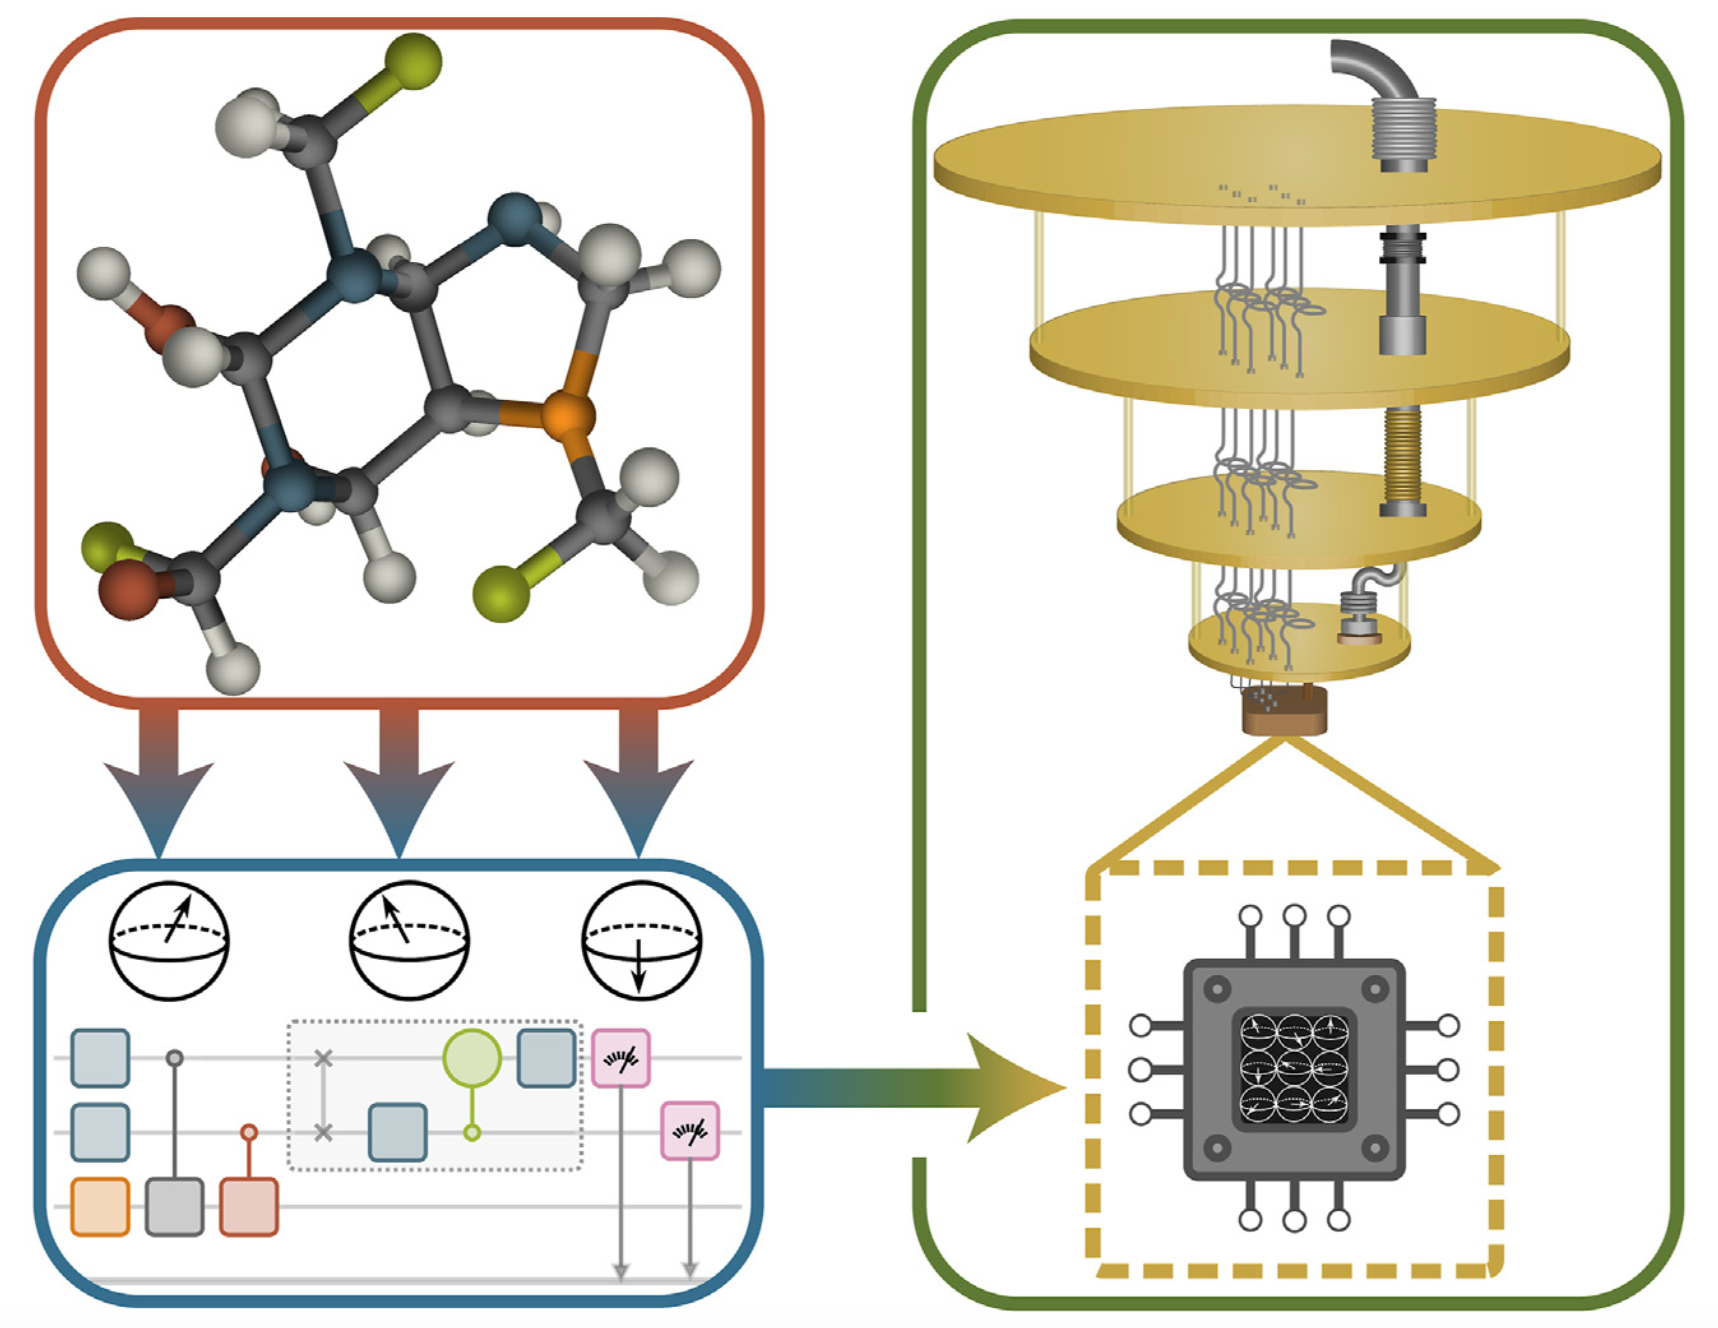
\includegraphics[width=.5\linewidth]{Immagini/Capitolo_0/qpu_chemistry.png}
        \caption{Illustrazione di una simulazione di chimica su quantum computer \cite{weidman_2024}.}
        \label{fig:qpu-chemistry}
    \end{minipage} \\[1ex]
    \begin{minipage}{.854\linewidth}
        \footnotesize
        Per calcolare una proprietà del sistema molecolare d'interesse (in alto a sinistra) si sceglie un metodo di calcolo, rappresentato con un diagramma (in basso a sinistra) che raffigura le operazioni quantistiche da svolgere su un set di qubit. Una volta costruito, il circuito quantistico è inviato ad un processore quantistico (a destra), contenuto all'interno di un criostato a temperature vicine ai 10 mK.
    \end{minipage}
\end{figure}

Un caso emblematico di difficoltà per la chimica computazionale classica è il calcolo delle interazioni elettroniche in molecole complesse. Descrivere il comportamento degli elettroni richiede approssimazioni che, spesso, sacrificano la precisione per contenere i costi computazionali. Al contrario, i computer quantistici - almeno in linea teorica - possono risolvere problemi che richiederebbero risorse esponenziali su hardware classico, anche utilizzando i migliori algoritmi disponibili.

Tuttavia, le implementazioni fisiche di questi dispositivi sono ancora in una fase embrionale e non sono ancora in grado di superare i computer classici in applicazioni pratiche. Nonostante ciò, in questo periodo caratterizzato da limiti hardware - spesso definito \textbf{era NISQ} (\inglese{Noisy Intermediate-Scale Quantum}) - lo sviluppo di software quantistico applicato alla chimica è un settore di ricerca in rapida evoluzione. Una delle direzioni più promettenti per rendere i calcoli quantistici applicabili alla simulazione di sistemi chimici nell'era NISQ è lo sviluppo di algoritmi \textbf{ibridi} che combinano metodi classici e quantistici.

Il \inglese{Variational Quantum Eigensolver} (VQE) \cite{Peruzzo_2014} rappresenta un esempio di approccio ibrido, progettato per adattarsi alle limitazioni tecnologiche dell’era NISQ. Il VQE sfrutta circuiti quantistici per stimare l’energia di stato fondamentale di un sistema molecolare, combinando simulazioni quantistiche e ottimizzazioni classiche. In questo lavoro, tale metodo è stato impiegato per confrontare differenti configurazioni di \textbf{ansatze}, con un’analisi comparativa delle loro prestazioni.

Resta da sottolineare che gli algoritmi quantistici appartengono a una classe differente e dovrebbero essere valutati attraverso metriche che non hanno un diretto analogo classico. Tra queste, ad esempio, ci sono la larghezza del circuito (numero di qubit), la profondità del circuito (numero di livelli di operazioni non commutanti) e il numero di misurazioni necessarie per ottenere quantità utili. 

In conclusione, le simulazioni di chimica quantistica, illustrate in Figura~\ref{fig:qpu-chemistry}, non solo rappresentano uno strumento avanzato per studiare le proprietà molecolari, ma costituiscono anche una piattaforma per testare le tecnologie quantistiche emergenti. Queste applicazioni permettono di esplorare i limiti attuali del calcolo quantistico, aprendo nuove opportunità per affrontare sfide scientifiche e tecnologiche di primaria importanza.

L’elaborato è strutturato per fornire un quadro d'insieme essenziale alla comprensione del metodo VQE e del suo contesto applicativo. Si parte dall’analisi dei concetti fondamentali della chimica computazionale classica, quindi si introducono i principi della computazione quantistica. Questo percorso teorico prepara il terreno per l’analisi delle simulazioni e dei risultati ottenuti, affrontati nelle sezioni successive.

% Capitolo 1
\chapter{Cenni teorici}

Questo capitolo offre una panoramica dei concetti e delle tecniche principali della \textbf{chimica computazionale}, un ramo della chimica che utilizza modelli matematici e algoritmi numerici per risolvere problemi legati alla struttura, alle proprietà e al comportamento delle molecole e dei materiali. Con l’avanzamento delle strategie computazionali e l’aumento della potenza di calcolo, la chimica computazionale è diventata uno strumento fondamentale per comprendere e prevedere fenomeni chimici.

In particolare, si affronteranno il metodo di Hartree-Fock e i metodi di correlazione elettronica \inglese{Full Configuration Interaction} e \inglese{Coupled-Cluster}, che permettono di descrivere le interazioni tra gli elettroni nelle molecole.

% ==============================================================================================================
\section{Problema elettronico}\label{sez:problema-elettronico}

Il problema affrontato nel presente elaborato è trovare soluzioni approssimate all'equazione di Schrödinger stazionaria non-relativistica

\begin{equation}\label{eqn:Schrödinger-stazionaria}
    \hat{H}\ket{\psi(\{\vec{R}_A\},\{\vec{r}_i\})} = E\ket{\psi(\{\vec{R}_A\},\{\vec{r}_i\})}
\end{equation}

dove $\hat{H}$ è l'hamiltoniana di un sistema di $N$ nuclei e $M$ elettroni, individuati rispettivamente dalle posizioni $\{\vec{R}_A\}_{A=1,\ldots,N}$ e $\{\vec{r}_i\}_{i=1,\ldots,M}$. Esplicitando le interazioni tra i componenti del sistema:

\begin{equation}\label{eqn:hamiltoniana-molecolare}
    \hat{H} = \hat{T}_e + \hat{T}_n + U_{nn} + U_{ee} + U_{ne}
\end{equation}

In cui compaiono i seguenti termini:

\begin{subequations}
\begin{itemize}
    \item [$\hat{T}_{e}$:] Operatore energia cinetica degli elettroni
        \begin{equation}\label{eqn:cinetica-elettroni}
            \hat{T}_{n} = \sum_{i}^{M} \frac{\,\hat{\vec{p}}_{i}^{2}}{m_e}
        \end{equation}

    \item [$\hat{T}_{n}$:] Operatore energia cinetica dei nuclei
        \begin{equation}\label{eqn:cinetica-nuclei}
            \hat{T}_{e} = \sum_{A}^{N} \frac{\,\hat{\vec{p}}_{A}^{2}}{M_A}
        \end{equation}
    
    \item [$U_{nn}$:] Energia potenziale coulombiana tra i nuclei
        \begin{equation}\label{eqn:potenziale-nuclei}
            U_{nn}(\{\vec{R}_A\})  = \frac12\sum_{A}^{N}\sum_{B\neq A}^{N} 
            \frac{1}{4\pi\varepsilon_0} \frac{Z_A Z_B e^2}{|\,\vec{R}_A - \vec{R}_B |}
        \end{equation}

    \item [$U_{ee}$:] Energia potenziale coulombiana tra gli elettroni
        \begin{equation}\label{eqn:potenziale-elettroni}
            U_{ee}(\{\vec{r}_i\}) = \frac12\sum_{i}^{M}\sum_{j\neq i}^{M} 
            \frac{1}{4\pi\varepsilon_0} \frac{e^2}{|\,\vec{r}_i - \vec{r}_j |}
        \end{equation}
    
    \item [$U_{en}$:] Energia potenziale coulombiana tra i gli elettroni e i nuclei
        \begin{equation}\label{eqn:potenziale-elettroni-nuclei}
            U_{en}(\{\vec{r}_i,\vec{R}_A\}) = -\sum_{A}^{N}\sum_{i}^{M} 
            \frac{1}{4\pi\varepsilon_0} \frac{Z_A e^2}{|\,\vec{R}_A - \vec{r}_i |}
        \end{equation}
\end{itemize}
\end{subequations}

Dove $\hat{\vec{p}}=-i\hbar\vec{\nabla}$ è l'operatore momento lineare, $m_e$ la massa dell'elettrone mentre $M_A$ quella del nucleo $A$ con numero atomico $Z_A$.

La presenza del termine $U_{en}$ porta subito ad una considerazione: qualsiasi soluzione \textbf{esatta} $\Psi(\{\vec{r}_i\},\{\vec{R}_A\})$ dell'equazione di Schrödinger non può essere fattorizzata in una parte elettronica e una nucleare \cite{Echenique_2007}.

\begin{equation*}
    \nexists\ \psi_n,\, \psi_{el}\, \text{ t.c. }
    \Psi(\{\vec{x}_i\},\{\vec{R}_A\}) = \psi_n(\{\vec{R}_A\})\ \psi_{el}(\{\vec{r}_i\})
\end{equation*}

Se ciò fosse possibile, il problema degli elettroni e quello dei nuclei potrebbero essere trattati separatamente. Da questa prima osservazione deriva l'utilità di introdurre un'approssimazione che riesca a slegare le due questioni.  
  
% --------------------------------------------------------------------------------------------------------------
\subsection{Approssimazione di Born-Oppenheimer}\label{subsec:Born-Oppenheimer}

Per affrontare il tema presentato alla Sezione~\ref{sez:problema-elettronico}, si parte con l'isolare i termini elettronici dal problema globale, costruendo un'hamiltoniana che dipende soltanto parametricamente dalle posizioni dei nuclei. 

\begin{equation}\label{eqn:hamiltoniana-elettronica}
    \hat{H}_{el} \ket{\psi_{el}} = 
    \left( \hat{T}_e + U_{ee} + U_{nn} + U_{ne} \right) \ket{\psi_{el}} =
    E(\{\vec{R}_A\}) \ket{\psi_{el}}
\end{equation}

Gli autostati $\ket{\psi_{el}}$ formano un sistema ortonormale completo, perciò le soluzioni del problema complessivo possono essere espresse come loro combinazioni lineari, pesate da delle funzioni parametriche $\chi(\{\vec{R}_A\})$ \cite{Sherril_2005}, che si occupano di modulare le diverse configurazioni elettroniche in relazione alla disposizione spaziale degli atomi nel sistema.

\begin{equation} \label{eqn:combinazione-stati-elettronici}
    \psi = \sum_{k} \chi_k(\{\vec{R}_A\})\ {\psi_{el}}_k(\{\vec{r}_i\},\{\vec{R}_A\})
\end{equation}

Questo rientra nell’approssimazione di Born-Oppenheimer \cite{Born_Opp}, che separa il problema elettronico da quello nucleare sfruttando la notevole differenza di massa tra nuclei ed elettroni. Essendo questi ultimi molto meno massivi, la loro dinamica avviene su scale temporali estremamente più brevi; ciò permette di assumere che, al variare della configurazione nucleare, gli elettroni adeguino istantaneamente il loro stato, seguendo il moto dei nuclei in modo adiabatico. 
Secondo questa interpretazione, vengono applicati i seguenti passaggi:

\begin{enumerate}
    \item La somma \ref{eqn:combinazione-stati-elettronici} si riduce ad un solo stato elettronico:
        \begin{equation}\label{eqn:approssimazione-adiabatica}
            \psi \approx \chi(\{\vec{R}_A\}) \psi_{el}(\{\vec{r}_i\},\{\vec{R}_A\})
        \end{equation}
        Si può quindi riscrivere l'equazione~(\ref{eqn:Schrödinger-stazionaria})
        \begin{equation}
            \left(\hat{T}_n+\hat{H}_e\right)\ket{\chi\psi_{el}} =
            \left(\hat{T}_n+E_{el}(\{\vec{R}_A\})\right)\ket{\chi\psi_{el}} = E\ket{\chi\psi_{el}}
        \end{equation}

    \item Il termine ottenuto applicando l'operatore $\hat{T}_n$ a $\psi_{el}$ diventa trascurabile, rendendo $\psi_{el}$ un semplice fattore moltiplicativo che può essere eliso:
        \begin{equation}
            (\hat{T}_n+E_{el})\chi = E\chi
        \end{equation}
\end{enumerate}

Adottando questo approccio, si ottiene un problema nucleare che dipende dal potenziale efficace $E_{el}(\{R_A\})$, assegnato dalla soluzione del problema elettronico parametrico nelle posizioni dei nuclei e indipendente dal loro moto. 
In sintesi: l'approssimazione di Born-Oppenheimer permette di studiare un sistema molecolare affrontando separatamente le dinamiche degli elettroni e dei nuclei. Questo lavoro di tesi si concentra prevalentemente sulle tecniche computazionali adottate per la costruzione di $E_{el}(\{R_A\})$.

% --------------------------------------------------------------------------------------------------------------
\subsection{Metodo di Hartree}\label{subsec:Hartree}

Assumendo valida l’approssimazione di Born-Oppenheimer, il tema principale diventa trovare lo stato fondamentale dell’hamiltoniana elettronica (eq. \ref{eqn:hamiltoniana-elettronica}) per una configurazione nucleare fissata $\{R_A\}$.

Nella risoluzione del problema elettronico - fatta eccezione per pochi casi semplici - ci si trova spesso a considerare problemi a molti elettroni, in cui la presenza del termine d'interazione $U_{ee}$ rende necessario introdurre un nuovo livello di approssimazione.

Un primo approccio è costituito dal metodo di Hartree, in cui è centrale il concetto di \textbf{approssimazione di campo medio}. In questo schema, ciascun elettrone viene trattato come se si muovesse all'interno del campo medio generato dagli altri elettroni in \inglese{background}, evitando di considerarne individualmente l'influenza. 
Se si immagina la densità di probabilità $|\psi_i({\vec{r}})|^2$ alla stregua di una distribuzione continua di carica, si può definire il \textbf{potenziale di Hartree} $U_H$:

\begin{equation}\label{eqn:distribuzione-di-carica}
    \rho_{k}^{(0)}(\vec{r}) = \sum_{i \neq k} \rho_{i}^{(0)}(\vec{r}) = 
    \sum_{i \neq k} e |\psi_{i}^{(0)}(\vec{r})|^2
\end{equation}
che dà:
\begin{equation}\label{eqn:potenziale-di-Hartree}
    {U_{H}}^{k}(\vec{r}) = -\frac{e}{4\pi\varepsilon_0}
    \frac12\int \frac{\rho_{k}^{(0)}(\vec{r'})}{|\,\vec{r}-\vec{r}'|} \d{\vec{r'}}
\end{equation}

A questo punto occorre fare una precisazione: le funzioni d'onda $\psi_i({\vec{r}})$, necessarie per determinare il potenziale di Hartree, sono le soluzioni del problema stesso e non è possibile conoscerle a priori. Per questo motivo, il metodo di Hartree rientra nelle cosiddette teorie auto-consistenti di campo medio o \inglese{self-consistent field} (SCF) \inglese{theories}. 
In breve, lo schema prevede di inserire inizialmente un \inglese{guess} o \textbf{ansatz} $\psi_{i}^{(0)}(\vec{r})$\footnote{Tipicamente, se si applica il metodo a sistemi atomici, le funzioni d'onda idrogenoidi} per calcolare in prima istanza $U_{H}^{(0)}$; dopodiché il metodo si sviluppa in maniera iterativa: ad ogni applicazione $m$-esima, si calcolano nuove soluzioni $\psi_{i}^{(m+1)}(\vec{r})$ e si determina il nuovo potenziale $U_{H}^{(m+1)}$, interrompendo il processo quando si raggiunge l'accuratezza desiderata\footnote{Nelle righe seguenti si trascurano gli indici d'iterazione $(m)$, poiché si preferisce presentare il metodo di Hartree in maniera sintetica.}. 

In tale impostazione l'hamiltoniana $H_{el}$ diventa separabile \cite{modern_quantum_chem}, perciò può essere scritta come somma delle hamiltoniane di singola particella $h_k$:

\begin{equation}\label{eqn:hamiltoniana-separabile}
    H_{el} \approx \sum_{k}^{M} h_{k}
\end{equation}

dove si introduce $U_H$ al posto di $U_{ee}$

\begin{equation}
    {U_{ee}}^{k} = \sum_{j \neq k}^{M} \frac{1}{4\pi\varepsilon_0} \frac{e^2}{|\,\vec{r}_k - \vec{r}_j |}
    \;\longrightarrow\;
    {V_{H}}^{k}
\end{equation}
per cui\footnote{Fissando la posizione dei nuclei il termine $U_{nn}$ diviene una semplice costante che introduce uno slittamento uniforme delle energie, motivo per cui viene omesso nel prosieguo della trattazione.}:
\begin{equation}\label{eqn:hamiltoniana-singola-particella}
    h_{k} = \frac{|\,\hat{\vec{p}}_k|^2}{2m_e} + 
    {U_{H}}^{k} + U_{en}^{k}
\end{equation}

% U_{en}^{k}
% \sum_{A}^{N} \frac{1}{4\pi\varepsilon_0} \frac{Z_A e^2}{| \vec{R}_A - \vec{r}_k |}

e si avrà che l'autovalore $E_{el}$ del problema elettronico è somma delle singole energie $\epsilon_k$ e la funzione d'onda del sistema $\psi_{el}$ è fattorizzabile nelle specifiche $\psi_k$

\begin{equation}\label{eqn:prodotto-di-Hartree}
    E_{el} = \sum_{k}^{M} \epsilon_k\ \ \land\ \ 
    \psi_{el} = \prod_{k}^{M} \psi_k
\end{equation}

nella letteratura, una $\psi_{el}$ costruita in questo modo è detta di frequente \textbf{prodotto di Hartree}.


% --------------------------------------------------------------------------------------------------------------
\subsection{Metodo di Hartree-Fock (HF)}\label{subsec:Hartree-Fock}

Lo schema di Hartree è alla base dei fondamenti teorici dei metodi SCF ma non è sufficiente per descrivere accuratamente i sistemi elettronici, poiché non tiene in considerazione un aspetto fondamentale della meccanica quantistica: l'\textbf{indistinguibilità} delle particelle \cite{computational_chem}.
Il prodotto di Hartree (eq. \ref{eqn:prodotto-di-Hartree}) non soddisfa la condizione di \textbf{antisimmetrizzazione}, per la quale è richiesto che ogni funzione d'onda che descrive un sistema di fermioni identici sia antisimmetrica rispetto allo scambio di ciascuna coppia di particelle \cite{Sherrill_2000}.
La correzione a questo problema fu proposta indipendentemente da Fock e Slater nel 1930 e consiste nell'introdurre una funzione d'onda a molti elettroni espressa tramite un \textbf{determinante di Slater} \cite{Echenique_2007}. Da questa idea, combinata l'approssimazione di campo medio ereditata dal metodo di Hartree, nasce il metodo di Hartree-Fock (HF).

% ..............................................................................................................
\subsubsection{Determinante di Slater}

Nel seguito della trattazione verrà effettuata una piccola variazione nella notazione: fino ad ora si sono indicati con $\psi(\vec{r})$ gli \textbf{orbitali spaziali}; da questo momento in poi, diventa opportuno considerare gli \textbf{orbitali di spin} $\phi({\vec{x}})$:

\begin{equation}\label{eqn:orbitale-di-spin}
    \phi(\vec{x}) = \psi(\vec{r})\,\nu
\end{equation}

in cui $\vec{x}=(\vec{r},\nu)$ e $\nu\in\{\alpha,\beta\}$ indicizza l'autostato di spin. 

L'introduzione degli orbitali di spin è propedeutica alla definizione del determinante di Slater, un modo compatto e conveniente per costruire una funzione d'onda $\Phi$ totalmente antisimmetrica:

\begin{equation}\label{eqn:determinante-di-Slater}
    \Phi(\vec{x}_1,...,\vec{x}_M) = \frac{1}{M!}
    \left|
    \begin{matrix}
        \phi_1(\vec{x}_1) & \phi_2(\vec{x}_1) & \dots  & \phi_M(\vec{x}_1) \\
        \phi_1(\vec{x}_2) & \phi_2(\vec{x}_2) & \dots  & \phi_M(\vec{x}_2) \\
        \vdots            & \vdots            & \ddots & \vdots            \\
        \phi_1(\vec{x}_M) & \phi_2(\vec{x}_M) & \dots  & \phi_M(\vec{x}_M) 
    \end{matrix}
    \right|
\end{equation}

questa scrittura sfrutta le proprietà del determinante di una matrice, il cui segno viene invertito quando vengono scambiate due colonne. Inoltre, affinché il risultato sia diverso da zero, righe e colonne devono essere tutte \textbf{linearmente indipendenti}; ciò assicura anche il rispetto del \textbf{principio di esclusione di Pauli}, poiché un sistema con due fermioni identici individuati dalle stesse coordinate $\vec{x}$ darebbe luogo a due righe uguali.

Generalmente, si richiede anche che gli orbitali di spin siano ortonormali:

\begin{equation}\label{eqn:ortonormalità}
    \braket{\phi_i}{\phi_j} = \delta_{ij},\ \forall\ i,j\in[1,M]
\end{equation}

% ..............................................................................................................
\subsubsection{Potenziale di Fock}

Il passo cruciale nello schema di Hartree-Fock è supporre che la soluzione del problema elettronico sia un singolo determinante di Slater, su cui l'energia è data da:

\begin{equation}\label{eqn:valore-di-aspettazione}
    \bra{\Phi}H_{el}\ket{\Phi}
\end{equation}

sinteticamente, si può dire che il metodo di Hartree-Fock aderisce alle stesse logiche dello schema di Hartree (sez. \ref{subsec:Hartree}) con lo scopo di minimizzare l'energia (eq. \ref{eqn:valore-di-aspettazione}), ma vede l'aggiunta del \textbf{potenziale di Fock}:

\begin{equation}\label{eqn:potenziale-di-Fock}
    {U_{F}}^k(\vec{x})\ket{\phi_i(\vec{x})} = 
    \left(
        \frac{e^2}{4\pi\varepsilon_0}
        \int \sum_{k}^{M} 
        \frac{\phi^{\star}_{k}(\vec{x}')\phi_{i}(\vec{x}')}{|\,\vec{r}_i - \vec{r}_k |}
        \ \d\vec{x}' 
    \right)
    \ket{\phi_k(\vec{x})}
\end{equation}

oltre alla scrittura aggiornata del potenziale di Hartree (eq. \ref{eqn:potenziale-di-Hartree})

\begin{equation}\label{eqn:potenziale-di-Hartree-HF}
    {U_{H}}^k(\vec{x})\ket{\phi_i(\vec{x})} = 
    \left(
        \frac{e^2}{4\pi\varepsilon_0}
        \int \sum_{k}^{M} 
        \frac{\phi^{\star}_{k}(\vec{x}')\phi_{k}(\vec{x}')}{|\,\vec{r}_i - \vec{r}_k |}
        \ \d\vec{x}' 
    \right)
    \ket{\phi_i(\vec{x})}
\end{equation}

infine, spesso si riassume l'equazione agli autovalori - di singola particella - utilizzando l'\textbf{operatore di Fock} $\hat{F}$:

\begin{equation}\label{eqn:operatore-di-Fock}
    \hat{F}^k = h_k + {U_H}^k - {U_F}^k
\end{equation}

con cui si scrive:

\begin{equation}\label{eqn:equazione-Hartree-Fock}
    \hat{F}^k \ket{\phi_k} = \epsilon_k \ket{\phi_k}
\end{equation}

% --------------------------------------------------------------------------------------------------------------
\subsection{Basi per gli orbitali molecolari}\label{subsec:basi}

Finora, non si è discusso di come esprimere concretamente la funzione d’onda, ma è importante sottolineare che $\Psi$  appartiene allo spazio di Hilbert $\mathcal{H} = L^2(\mathbb{R}^3) \times \mathbb{C}^2$ , che è uno spazio infinito dimensionale. Per poterla trattare numericamente, è necessario svilupparla su una base che, pur essendo finita, permetta di ottenerne una rappresentazione approssimata. La selezione della base è dunque essenziale per bilanciare la precisione della descrizione e la complessità computazionale del sistema.

Questo tema fu affrontato inizialmente nel 1951 da Roothaan, che propose di rappresentare gli orbitali molecolari come combinazioni lineari finite di \textbf{funzioni di base} $\{\chi_\nu\}$\footnote{Si adotterà la pratica, comune in letteratura, di associare indici latini agli orbitali molecolari e indici greci a quelli atomici}, spesso chiamate \textbf{orbitali atomici}:

\begin{equation}\label{eqn:LCAO}
    \phi_k \approx \sum_{\nu}^{} c_{\nu k}\chi_\nu
\end{equation}

dove $c_\nu$ sono i coefficienti della combinazione lineare. Tipicamente, nel'effettuare calcoli su sistemi atomici, si utilizzano come ansatz le funzioni d'onda idrogenoidi $\chi_{n\ell m}^{Z}$, che derivano dalla soluzione dell'unico problema molecolare risolvibile analiticamente.
Storicamente, nelle prime versioni della teoria degli orbitali molecolari, furono proprio queste ad essere proposte come orbitali atomici per la costruzione delle funzioni $\phi_k$ \cite{Pople_1998}. Diventò consuetudine scegliere funzioni centrate sui nuclei atomici che richiamassero le $\chi_{n\ell m}^{Z}$ e fu in questo spirito che si iniziò ad utilizzare i \inglese{Slater-Type Orbitals} (STO) \cite{Echenique_2007}:

\begin{equation}\label{eqn:STO}
    \chi^{\text{STO}}_{a,b,c,\zeta} = N_{a,b,c} x^a y^b z^c e^{-\zeta |\vec{r}|}
\end{equation}

%\chi^{\text{STO}}_{\nu} (\vec{r},\vec{{R}_A}_\nu) = N^{\text{STO}}_{\nu} \tilde{Y}_{\ell_\nu m_\nu}^{c,s} ({\theta_A}_\nu,{\varphi_A}_\nu)|\vec{r}-{\vec{R}_A}_\nu|^{n_\nu-1} e^{-\zeta_\nu|\vec{r}-{\vec{R}_A}_\nu|}
% $\tilde{Y}_{\ell_\nu m_\nu}^{c,s}$ delle armoniche sferiche modificate \cite{Echenique_2007}. 

dove $N^{\text{STO}}_{a,b,c}$ è la costante di normalizzazione, $\zeta$ un parametro e $a,b,c$ sono legate al momento angolare.
Queste funzioni mostrano gli stessi comportamenti asintotici delle $\chi_{n\ell m}^{Z}$ a corto e lungo raggio, rispettando le condizioni imposte dalla teoria, tuttavia presentano importanti svantaggi computazionali: gli integrali coinvolti nel calcolo del valore di aspettazione (eq. \ref{eqn:valore-di-aspettazione}) richiedono un grande sforzo in termini di tempo. Ciò rese impossibile l'implementazione delle STO nelle simulazioni di grandi molecole.

La successiva introduzione delle funzioni gaussiane o \inglese{Gaussian-Type Orbitals} (GTO) fu un'importante sviluppo poiché, sacrificando alcune proprietà teoriche, permettevano di semplificare, e insieme velocizzare, i calcoli degli integrali.

\begin{equation}\label{eqn:GTO}
    \chi^{\text{GTO}}_{a,b,c,\zeta} = N_{a,b,c} x^a y^b z^c e^{-\zeta |\vec{r}|^2}
\end{equation}

In particolare, grazie al grande vantaggio computazionale, possono essere usate in quantità maggiore per sopperire alla loro inesattezza fisica. Pertanto, per combinare i pregi di STO e GTO, furono introdotte le funzioni gaussiane contratte o \inglese{Contracted GTO} (CGTO), che utilizzano un certo numero $n$ di funzioni gaussiane per approssimare una funzione di Slater:

\begin{equation}\label{eqn:CGTO}
    \chi^{\text{CGTO}}_{a,b,c,\zeta} = N_{a,b,c} x^a y^b z^c 
    \sum_{i}^{n} e^{-\zeta_i |\vec{r}|^2}
\end{equation}

Infine, da queste funzioni nacque la famiglia di basi STO-$n$G, in cui ciascuna CGTO è costruita a partire da $n$ GTO. Al crescere del numero di funzioni gaussiane utilizzate aumenta l'accuratezza raggiunta dal calcolo, ma al prezzo di un più elevato tempo di esecuzione.
Le simulazioni svolte nel contesto di questo elaborato saranno principalmente orientate ad uno studio qualitativo perciò, nella stragrande maggioranza dei casi, si utilizzerà la base STO-3G.



% ==============================================================================================================
\section{Seconda quantizzazione}\label{sez:seconda-quantizzazione}

In questo elaborato, così come nella letteratura, si fa spesso uso del formalismo di \textbf{seconda quantizzazione}, una formulazione della meccanica quantistica che facilita la descrizione dei sistemi a molti corpi. Se nella \textbf{prima} quantizzazione sono le variabili, come posizione e momento, a essere promosse ad operatori quantistici, nella seconda sono i campi stessi a essere \textbf{quantizzati}. Senza addentrarsi ulteriormente nei dettagli, l’idea è di considerare le particelle come eccitazioni fondamentali dei campi stessi; in questo senso, l’occupazione degli orbitali viene rappresentata tramite operatori di creazione e annichilazione, che aggiungono o rimuovono particelle dagli stati. Ne consegue che il numero di particelle nel sistema non è fissato, caratteristica che rappresenta l'elemento di novità fondamentale di questa notazione \cite{second_q}.

% --------------------------------------------------------------------------------------------------------------
\subsection{Spazio di Fock}

Considerando questa descrizione, si introduce lo spazio di Fock $\mathcal{F}$ come una generalizzazione dello spazio di Hilbert, che permette di rappresentare stati con numero di particelle variabile. Si pensi innanzitutto agli elementi di $\mathcal{F}$: gli stati di Fock $\ket{f}$, che possono essere descritti tramite l'occupazione di ciascuno stato di singola particella. Se $n_\alpha\in\mathbb{N}$ è il numero di particelle in $\ket{\alpha}$ con $\alpha=1,2,...$ che indicizza lo stato

\begin{equation}\label{eqn:stato-di-Fock}
    \ket{f} = \ket{n_1 n_2 n_3 ...}
\end{equation}

Nel caso fermionico, uno stato $\ket{\alpha}$, caratterizzato da un proprio set di numeri quantici, può essere occupato al più da una particella, perciò: $n_\alpha\in\{0,1\}$. 
Ad esempio, si considerino gli orbitali di spin (eq. \ref{eqn:orbitale-di-spin}): per indicare comodamente lo stato di occupazione dei $\phi_i$ si può adottare la notazione:

\begin{equation}\label{eqn:notazione-ket}
    \ket{j k \dots l} \equiv \ket{\phi_j \phi_k \dots \phi_l}
\end{equation}

Insomma, lo spazio di Fock $\mathcal{F}$ è lo spazio in cui vivono tutti i possibili stati di Fock $\ket{f}$, cioè tutte le configurazioni generabili a partire dal set dei $\{\phi_i\}$; se si hanno $2K$ orbitali di spin, si avrà che $\dim{(\mathcal{F})} = 2^{2K}$.

% --------------------------------------------------------------------------------------------------------------
\subsection{Operatori fermionici di creazione e distruzione}

Se con $\ket{0}$ si indica lo \textbf{stato di vuoto}, si possono introdurre gli operatori creazione e distruzione:

\begin{equation}\label{eqn:creazione-distruzione}
\begin{cases}
    a^{\dagger}_{i} \ket{0} = \ket{i}\\
    a_i \ket{j} = \delta_{i j}\ket{0}
\end{cases}
\end{equation}

$a^{\dagger}_{i}$ agisce sullo stato di vuoto \textbf{creando} un elettrone nello stato $\ket{i}$; $a_i$ agisce su uno stato occupato $\ket{j}$ \textbf{distruggendo} l'elettrone quando $j=i$, altrimenti restituisce zero.

Equivalentemente, sullo stato $\ket{j k \dots l}$:

\begin{equation}
\begin{cases}
    a^{\dagger}_{i} \ket{j k \dots l} = \ket{i j k \dots l}\\
    a_i \ket{i j k \dots l} = \ket{j k \dots l}
\end{cases}
\end{equation}

Su particelle di natura fermionica rispettano le condizioni richieste dalla teoria:

\begin{enumerate}
    \item \textbf{Antisimmetria} L'ordine in cui sono applicati due operatori di creazione è determinante: 
    \begin{subequations}\label{eqn:antisimmetria-operatori-fermionici}
        \begin{equation}
            a^{\dagger}_{i} a^{\dagger}_{j} \ket{k \dots l} = \ket{i j k \dots l}
        \end{equation}
        mentre
        \begin{equation}
            a^{\dagger}_{j} a^{\dagger}_{i} \ket{k \dots l} = \ket{j i k \dots l} = - \ket{i j k \dots l}
        \end{equation}
        riassumendo:
        \begin{equation}
            a^{\dagger}_{i} a^{\dagger}_{j} \ket{0} = 
            - a^{\dagger}_{j} a^{\dagger}_{i} \ket{0} = \ket{i j}
        \end{equation}
    \end{subequations}

    \item \textbf{Esclusione} Non è possibile creare due elettroni nello stesso stato $\ket{i}$
    \begin{equation}
        a^{\dagger}_{i} a^{\dagger}_{i} \ket{0} = ( a^{\dagger}_{i})^2 \ket{0} = 0
    \end{equation}
\end{enumerate}


Con queste premesse si può definire l'operatore numero:

\begin{equation}\label{eqn:operatore-numero}
    \hat{n}_i = a^{\dagger}_{i} a_{i}
\end{equation}
    
i cui autovalori sono 0 e 1: 

\begin{equation}\label{eqn:autovalori-operatore-numero}
    \hat{n}_i \ket{i j k \dots l} = \ket{i j k \dots l}\\
    \hat{n}_i \ket{j k \dots l} = 0
\end{equation}

in altri termini, quando $\hat{n}_i$ agisce su uno stato di Fock restituisce zero se lo stato $\ket{i}$ non è occupato, altrimenti restituisce lo stato di Fock stesso.

% --------------------------------------------------------------------------------------------------------------
\subsection{Particelle non interagenti}

Si prenda un sistema di fermioni identici non interagenti. Supponendo di averne $M$, si può scrivere l'hamiltoniana del sistema

\begin{equation}\label{eqn:hamiltoniana-libera}
    \hat{H} = \sum_{i}^{M} \frac{|\,\hat{\vec{p}}\,|^2}{2m}
\end{equation}

Con il formalismo di seconda quantizzazione è possibile scrivere $\hat{H}$ senza specificare il numero di particelle; si possono ad esempio indicizzare i momenti $k$, sommando sui livelli energetici $\frac{k^2}{2m}$ pesati dal numero di particelle:

\begin{equation}\label{eqn:hamiltoniana-libera-seconda-q}
    \hat{H} = \sum_{k} \frac{k^2}{2m} a^{\dagger}_{k} a_{k}
\end{equation}

un'altra opzione è considerare l'hamiltoniana di singola particella $\hat{h}$ e supporre che possa essere diagonalizzata in questo modo:

\begin{equation}
    \hat{h} = \sum_{i} \epsilon_i\ \ket{i}\bra{i}
\end{equation}

che permette di scrivere:

\begin{equation}
    \hat{H} = \sum_{i} \epsilon_i\ a^{\dagger}_{i} a_{i}
\end{equation}

qui $a^{\dagger}_{i} a_{i}$ restituisce l'occupazione dello stato $\ket{i}$. L'hamiltoniana in sostanza è la somma delle possibili energie $\epsilon_i$ pesate dal numero di particelle.


% --------------------------------------------------------------------------------------------------------------
\subsection{Hamiltoniana di seconda quantizzazione}\label{subsec:hamiltoniana-seconda-q}

La forma dell’Hamiltoniana elettronica, che descrive il problema di interesse in questo lavoro, deriva direttamente dalle considerazioni esposte finora \cite{modern_quantum_chem}.

\begin{equation}\label{eqn:hamiltoniana-seconda-q}
    H_{el} = \sum_{p,q} h_{pq} a^{\dagger}_{p} a_{q} +
    \frac12 \sum_{p,q,r,s} g_{pqrs} a^{\dagger}_{p} a^{\dagger}_{q} a_{r} a_{s}
\end{equation}

Dove si sono introdotti due nuovi oggetti:

\begin{subequations}
\begin{itemize}
    \item[$\bf h_{pq}$] è l'integrale a un elettrone, che contiene l'energia cinetica e l'interazione coulombiana con i nuclei
    \begin{equation}\label{eqn:integrale-un-elettrone}
        h_{pq} \equiv \bra{p} \hat{T}_e + U_{en}(\vec{r}) \ket{q} = 
        \int \phi^{\star}_{p}(\vec{x})
        \left(
            \frac{\vec{p}^2}{2m_{e}} - \sum_{A} \frac{Z_A}{|\,\vec{R}_A-\vec{r}|}
        \right) \phi_{q}(\vec{x})\ \d{\vec{x}} 
    \end{equation}
    \item[$\bf g_{pqrs}$] è l'integrale a due elettroni, dovuto alla repulsione elettrone-elettrone 
    \begin{equation}\label{eqn:integrale-due-elettroni}
        h_{pqrs} \equiv \bra{pq} U_{ee}(\vec{r}_1,\vec{r}_2) \ket{rs} =
        \int 
        \frac{\phi^{\star}_{p}(\vec{x}_1)\phi^{\star}_{q}(\vec{x}_2)\phi_{r}(\vec{x}_1)\phi_{s}(\vec{x}_2)}
        {|\,\vec{r}_1 - \vec{r}_2|}\ \d{\vec{x}_1}\d{\vec{x}_2}
    \end{equation}
\end{itemize}
\end{subequations}

Poiché $H_{el}$ contiene somme con fino a quattro operatori creazione e distruzione indicizzati separatamente, se si andasse a costruirla a partire da $2K$ orbitali di spin, si otterrebbe un numero $\mathcal{O}(2K^4)$ di termini.

% ==============================================================================================================
\section{Metodi classici post Hartree-Fock}\label{sez:post-HF}

L’approssimazione di campo medio introduce un importante errore sistematico poiché, durante il suo moto, un elettrone non interagisce con una semplice distribuzione uniforme, ma viene istantaneamente influenzato dalla repulsione coulombiana dovuta a ciascuno degli altri. Questo comportamento è noto come \textbf{correlazione elettronica} ed è considerato la principale limitazione del metodo di Hartree-Fock (sez. \ref{subsec:Hartree-Fock}) \cite{computational_chem}.
La correlazione elettronica porta ad una diminuzione significativa dell'energia repulsiva tra gli elettroni, determinando un'energia elettronica minore di quella prevista da HF; diventa perciò necessario introdurre delle correzioni che possano prendere in considerazione questo fenomeno.

I metodi sviluppati per descrivere correttamente le interazioni tra elettroni sono detti \textbf{post-Hartree-Fock}. Tra questi, \inglese{Configuration Interaction} (CI) e \inglese{Coupled Cluster} (CC) spiccano, per ragioni diverse, in molte applicazioni della chimica quantistica.

% --------------------------------------------------------------------------------------------------------------
\subsection{Configuration Interaction (CI)}\label{subsec:configuration-interaction}

L'idea alla base della \inglese{configuration interaction} è migliorare la funzione d’onda HF aggiungendo termini che rappresentano la promozione degli elettroni dagli orbitali occupati a quelli virtuali. Ciascuno dei termini nella funzione d'onda CI rappresenta una configurazione elettronica specifica e la struttura elettronica del sistema viene interpretata come il risultato dell’interazione tra di esse.

Si supponga di studiare un problema molecolare con $M$ elettroni attraverso il metodo di Hartree-Fock, da cui si ottiene il set di $2K$ orbitali di spin $\{\ket{\phi_i}\}$. La funzione d'onda HF $\ket{\Phi_{\text{HF}}}$ è il determinante di Slater costruito a partire dagli $M$ orbitali di spin associati a energie minori, ma combinando diversamente i $\{\ket{\phi_i}\}$ - includendo quelli rimasti liberi~- si possono ottenere molti altri determinanti a $M$ particelle, detti \inglese{configuration state functions} (CSF). 
Ad esempio, con $\ket{\Phi_{a}^{r}}$ si indica il determinante di singola eccitazione, che differisce da $\ket{\Phi_{\text{HF}}}$ poiché l'orbitale di spin $\ket{\phi_a}$ viene sostituito da $\ket{\phi_r}$. Allo stesso modo, si possono definire il determinante di doppia eccitazione $\ket{\Phi_{ab}^{rs}}$, di terza $\ket{\Phi_{abc}^{rst}}$ e così via gli altri.
Insieme, queste funzioni d'onda a molti elettroni possono essere usate per espandere la soluzione esatta del problema elettronico \cite{computational_chem}:


\begin{subequations}\label{eqn:espansione-CI}
\begin{equation}
    \ket{\Psi} = c_0 \ket{\Phi_{\text{HF}}} + \sum_{a,r} c_{a}^{r} \ket{\Phi_{a}^{r}} +
    \sum_{\substack{a<b\\r<s}} c_{ab}^{rs} \ket{\Phi_{ab}^{rs}} + 
    \sum_{\substack{a<b<c\\r<s<t}} c_{abc}^{rst} \ket{\Phi_{abc}^{rst}} + \dots
\end{equation}

o, sfruttando il formalismo di seconda quantizzazione:

\begin{equation}
    \ket{\Psi} = c_0 \ket{\Phi_{\text{HF}}} + \sum_{a,r} c_{a}^{r}\, a_{a} a^{\dagger}_{r}\ket{\Phi_{\text{HF}}} +
    \sum_{\substack{a<b\\r<s}} c_{ab}^{rs}\, a_{a}a_{b} a^{\dagger}_{r}a^{\dagger}_{s} \ket{\Phi_{\text{HF}}} + 
    \sum_{\substack{a<b<c\\r<s<t}} c_{abc}^{rst}\,
    a_{a}a_{b}a_{c} a^{\dagger}_{r}a^{\dagger}_{s}a^{\dagger}_{t}  \ket{\Phi_{\text{HF}}} + \dots
\end{equation}
\end{subequations}

una volta costruita la $\ket{\Psi}$, parametrica nei coefficienti $c$, si può calcolare l'energia tramite il principio variazionale. 
Se tutte le CSF possibili vengono considerate il metodo CI fornisce risultati estremamente accurati e prende il nome \inglese{Full Configuration Interaction} (FCI); purtroppo, anche partendo da una base $\{\ket{\phi_i}\}$ incompleta, FCI diventa rapidamente intrattabile al crescere della complessità della molecola, rimanendo applicabile soltanto a sistemi molto semplici. 
Una comune approssimazione per ridurre il costo computazionale di FCI è la \inglese{Configuration Interaction Singles Doubles} (CISD), che consiste nel troncare l'espansione (eq. \ref{eqn:espansione-CI}) alle sole CSF di singola e doppia eccitazione; alcune sue varianti sono CISDT e CISDTQ, che aggiungono a CISD i determinanti di tripla e quadrupla eccitazione \cite{Sherrill_1995}. 
Altre implementazioni frequenti di CI sono i \inglese{Multi-Configurational SCF} (MCSCF), in cui si vanno ad ottimizzare anche i coefficienti LCAO (eq. \ref{eqn:LCAO}), e la variante \inglese{Complete Active Space SCF} (CASSCF), in cui si selezionano soltanto gli orbitali molecolari che contribuiscono maggiormente alla correlazione, gli \inglese{active orbitals}, per formare un \inglese{active space} di dimensioni ridotte.

Pur rappresentando delle alternative valide, le approssimazioni troncate di CI presentano un problema pratico che non può essere eluso: non soddisfano una proprietà fondamentale, la \inglese{size consistency}, cruciale per la corretta descrizione dei sistemi complessi.

% ..............................................................................................................
\subsubsection{Size Consistency}

Un metodo computazionale è detto \inglese{size-consistent} se permette di fattorizzare la funzione d'onda di un sistema - composto da sottosistemi non interagenti - come prodotto delle funzioni d'onda degli elementi che lo compongono, così da poter scrivere l'energia totale come la somma dei singoli frammenti \cite{Anand_2022}. Ad esempio, per due sistemi $A$ e $B$ infinitamente lontani, come gli atomi dissociati di una molecola, varrebbero lo relazioni:

\begin{equation}\label{eqn:size-consistency}
\begin{cases}
    \psi_{AB} = \ket{\psi_A\psi_B}\\
    E_{AB} = E_A + E_B
\end{cases}
\end{equation}

Dal momento che le tecniche CI appena discusse non godono di questa proprietà, diventa prioritario trovare un metodo con un costo computazionale contenuto che soddisfi anche la condizione di \inglese{size consistency}.

% --------------------------------------------------------------------------------------------------------------
\subsection{Coupled Cluster (CC)}\label{subsec:coupled-cluster}

I metodi \inglese{Coupled Cluster}, inizialmente introdotti nel 1960, godono della proprietà di \inglese{size consistency} e sono attualmente considerati il \inglese{golden standard} dei metodi computazionali per via del bilanciamento tra accuratezza e efficienza che offrono \cite{Anand_2022,Bartlett_2007}. 

L'idea alla base della teoria CC è descrivere la funzione d'onda di stato fondamentale applicando un operatore d'eccitazione $\hat{T}$ esponenziato su un determinante di riferimento, tipicamente lo stato di Hartree-Fock $\ket{\Phi_{\text{HF}}}$.

\begin{equation}\label{eqn:coupled-cluster}
    \ket{\Phi_{\text{CC}}} = e^{\hat{T}} \ket{\Phi_{\text{HF}}}
\end{equation}

$\hat{T}$ è detto \textbf{operatore di cluster} e la sua azione, in analogia con il metodo CI, è quella di restituire una combinazione lineare di determinanti. Nello specifico, $\hat{T}$ è la somma degli operatori relativi ai diversi ordini di eccitazione $\hat{T} = \hat{T}_1 + \hat{T}_2 + \dots$, dove:

\begin{subequations}\label{eqn:cluster-operator}
\begin{equation}\label{eqn:cluster-operator-singles}
    \hat{T}_1 = \sum_{a,r} \theta_{a}^{r}\, a^{\dagger}_r a_a
\end{equation}

\begin{equation}\label{eqn:cluster-operator-doubles}
    \hat{T}_2 = \sum_{\substack{a<b\\r<s}} \theta_{ab}^{rs}\, a^{\dagger}_r a^{\dagger}_{s} a_a a_b
\end{equation}
\end{subequations}

Tra gli aspetti vantaggiosi di CC vi è la possibilità di troncare sistematicamente $\hat{T}$ ad ordini minori; a seconda di quanti termini si includono nella somma si ottengono le varianti CCS, CCD, CCSD e così via:

\begin{subequations}\label{eqn:CC-variants}
\begin{align}
    \ket{\Phi_{\text{CCS}}}  &= e^{\hat{T}_1} \ket{\Phi_{\text{HF}}}
    \\
    \ket{\Phi_{\text{CCD}}}  &= e^{\hat{T}_2} \ket{\Phi_{\text{HF}}}
    \\
    \ket{\Phi_{\text{CCSD}}} &= e^{\hat{T}_1 + \hat{T}_2} \ket{\Phi_{\text{HF}}}
\end{align}
\end{subequations}

I vantaggi della teoria \inglese{Coupled Cluster} hanno un prezzo: il singolo determinante di riferimento rende i metodi CC non variazionali, ma la \inglese{size consistency} è ritenuta una questione di maggiore importanza \cite{Pople_1998}.

Vi è una variante significativa di CC, la \inglese{Unitary Coupled Cluster} (UCC), che consiste nel modificare la trasformazione $e^{\hat{T}}$ in modo da renderla unitaria:

\begin{equation}\label{eqn:unitary-coupled-cluster}
    \ket{\Phi_{\text{UCC}}} = e^{\hat{T}-\hat{T}^\dagger} \ket{\Phi_{\text{HF}}}
\end{equation}

quest'ultima è di particolare interesse perché, come verrà trattato in seguito (sez. \ref{sez:quantum-coupled-cluster}), può essere mappata in modo naturale su un circuito quantistico \cite{Sokolov_2020}.


% Capitolo 2

\chapter{Soluzioni computazionali quantistiche}

Dopo aver esplorato il problema elettronico e le tecniche classiche, l’emergere dei computer quantistici apre nuove prospettive per affrontare i sistemi chimici più complessi. In questo capitolo, si introducono i concetti fondamentali della computazione quantistica, come \textbf{qubit}, \textbf{gates} e \textbf{circuiti}, gettando le basi per approcci innovativi come gli algoritmi variazionali quantistici.


% ==============================================================================================================
\section{Introduzione al quantum computing}

% --------------------------------------------------------------------------------------------------------------
\subsection{Qubit}

Un \textbf{qubit} è un qualsiasi sistema fisico a due livelli, generalmente indicati con $\ket{0}$ e $\ket{1}$, e rappresenta l'unità fondamentale di informazione del quantum computing. 
Mentre un \inglese{bit} classico può assumere soltanto due valori, 0 oppure 1, un \inglese{quantum bit} può esistere in una sovrapposizione qualsiasi dei due stati \cite{FernandezCombarro2020,Nielsen_Chuang_2010}:

\begin{equation}\label{eqn:qubit}
    \ket{q} = \alpha \ket{0} + \beta \ket{1}
\end{equation}

dove $\alpha,\beta\in\mathbb{C}$ sono le ampiezze di probabilità dei due stati e pertanto soddisfano la condizione:

\begin{equation}\label{eqn:misura-unitaria}
    |\alpha|^2 + |\beta|^2 = 1
\end{equation}

% ..............................................................................................................
\subsubsection{Sfera di Bloch}

Attraverso semplici manipolazioni algebriche, rispettando la condizione di unitarietà (eq. \ref{eqn:misura-unitaria}) e considerando che una fase globale non ha un effetto fisico visibile, è possibile riscrivere la \ref{eqn:qubit}:

\begin{equation}\label{eqn:bloch}
    \ket{q} = \cos \frac{\theta}{2} \ket{0} + e^{i\varphi} \sin \frac{\theta}{2} \ket{1}
\end{equation}

questa relazione offre una comoda rappresentazione, che permette di visualizzare il qubit in maniera intuitiva: le variabili $\theta$ e $\phi$ individuano un punto nello spazio posizionato sulla superficie di una sfera unitaria, detta \textbf{sfera di Bloch}.

\begin{figure}[H]
    \centering
    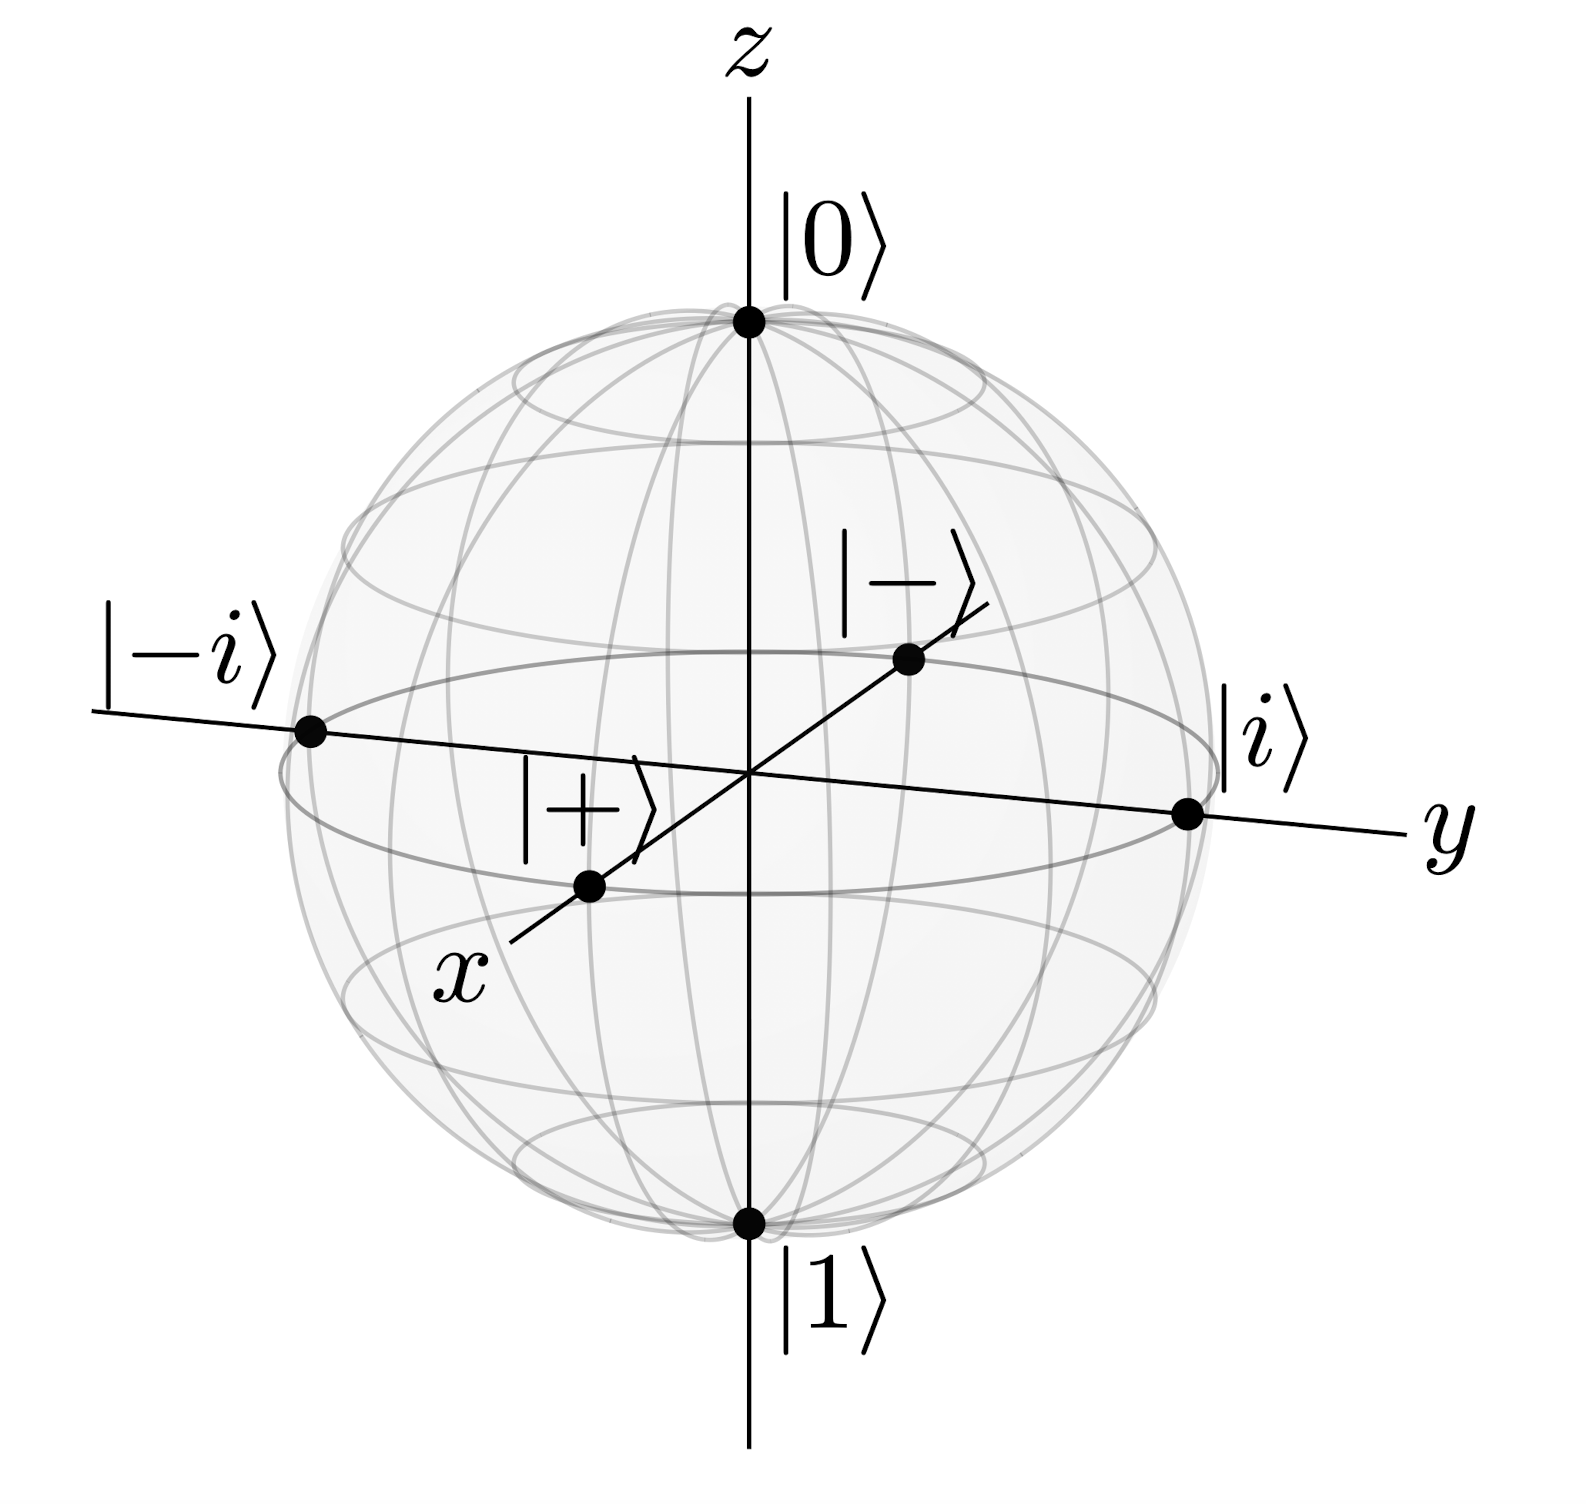
\includegraphics[width=0.5\textwidth]{Immagini/Capitolo_2/bloch.png}
    %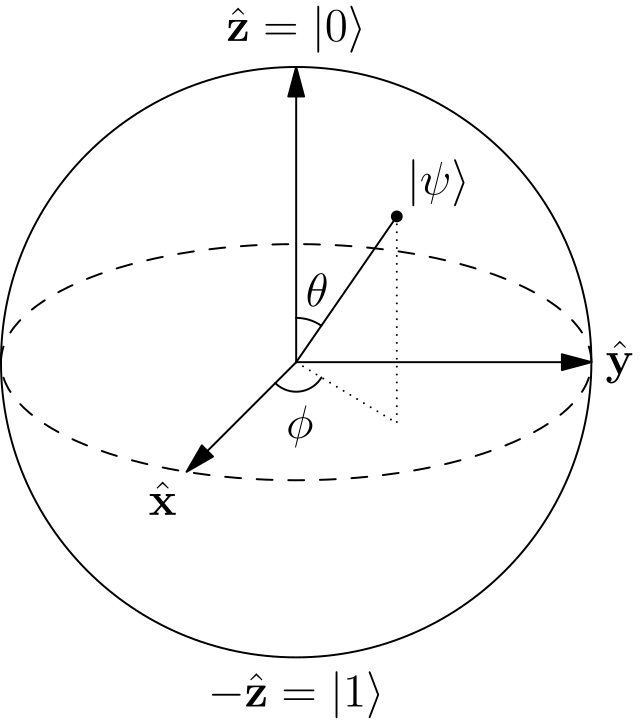
\includegraphics[width=0.5\textwidth]{Immagini/Capitolo_2/bloch.svg.png}
    \caption{Sfera di Bloch \cite{Wong2022}.}
    \label{fig:sfera-di-Bloch}
\end{figure} 

I punti ai poli della sfera sono identificati dagli stati $\ket{0}$, $\ket{1}$ che insieme formano la cosiddetta \textbf{base computazionale} $\{\ket{0},\ket{1}\}$. Allo stesso modo, i punti agli antipodi sugli assi $x$ e $y$ corrispondono ciascuno ad una base bidimensionale, spesso indicate con $\{\ket{+},\ket{-}\}$ e $\{\ket{+i},\ket{-i}\}$, i cui elementi possono essere sviluppati sulla base computazionale:

\begin{subequations}\label{eqn:autostati-rotazioni}
\small
\begin{align}
    &\ket{0} = \vectorTwo{1}{0} &&\ket{1} = \vectorTwo{0}{1}\\
    &\ket{+} = \frac{\ket{0}+\ket{1}}{\sqrt{2}} = \frac{1}{\sqrt{2}} \vectorTwo{1}{1} 
    &&\ket{-} = \frac{\ket{0}-\ket{1}}{\sqrt{2}} = \frac{1}{\sqrt{2}} \vectorTwo{1}{-1}\\
    &\ket{+i} = \frac{\ket{0}+i\ket{1}}{\sqrt{2}} = \frac{1}{\sqrt{2}} \vectorTwo{1}{i} 
    &&\ket{-i} = \frac{\ket{0}-i\ket{1}}{\sqrt{2}} = \frac{1}{\sqrt{2}} \vectorTwo{1}{-i}
\end{align}
\end{subequations}

% ..............................................................................................................
\subsubsection{Informazione di un qubit}

Per caratterizzare univocamente uno stato $\ket{q}$ occorrono due numeri reali indipendenti, che lo collocano in uno degli infiniti punti sulla sfera di Bloch; si potrebbe allora pensare che un qubit possa memorizzare una quantità di informazioni virtualmente illimitata. Tuttavia, per la natura quantistica del sistema, non è possibile estrarre i coefficienti $\alpha$ e $\beta$ con un numero finito di misure: quando si interroga una prima volta lo stato di sovrapposizione $\ket{q}$, esso collassa in uno stato definito, $\ket{0}$ o $\ket{1}$, ciascuno con una probabilità data dal modulo quadro della sua ampiezza, $|\alpha|^2$ o $|\beta|^2$. Da quel momento in poi, ogni misurazione successiva sullo stesso qubit restituirà sempre lo stesso risultato. 

%Eppure, proprio per via della sua natura probabilistica, il qubit offre una nuova modalità di calcolo: un sistema quantistico può esplorare una gamma di stati in parallelo, portando il quantum computing verso problemi che il calcolo classico fatica a risolvere.


% --------------------------------------------------------------------------------------------------------------
\subsection{Operazioni sui qubit}\label{subsec:gates}

Sui bit classici le operazioni vengono implementate tramite \inglese{logic gates}, quali AND, OR e NOT, e la loro azione viene schematizzata attraverso dei circuiti. Analogamente, le trasformazioni sui qubit sono compiute attraverso \inglese{quantum gates}, generalmente indicati con la lettera $U$, e vengono riassunte con dei \textbf{circuiti quantistici}. 

\begin{center}
\begin{quantikz}
    \lstick{$\ket{q}$} & \gate{U} & \rstick{$\ket{q'}$}
\end{quantikz}
\end{center}

Chiaramente, l'applicazione di un gate quantistico $U$ ad uno stato $\ket{q}$ deve restituire uno stato $\ket{q'}$ valido: la condizione \ref{eqn:misura-unitaria} deve rimanere soddisfatta. $U$, insomma, agisce sui qubit come un operatore \textbf{unitario} ($UU^{\dagger}=\mathbb{I}$) e può essere anche espresso in forma matriciale.
Di seguito vengono esposti alcuni dei principali \inglese{quantum gates}.

% ..............................................................................................................
\subsubsection{X gate (NOT)}

\begin{center}
\begin{quantikz}
    & \gate{X} &
\end{quantikz}
\end{center}

La sua rappresentazione matriciale è:

\begin{equation}
X \equiv
\begin{pmatrix}
    0 &1\\
    1 &0
\end{pmatrix}
\end{equation}

è considerato l'analogo del NOT gate classico, perché agisce sullo stato $\ket{1}$ mandandolo in $\ket{0}$ e viceversa:

\begin{center}
\begin{quantikz}
    \lstick{$\ket{0}$} & \gate{X} & \rstick{$\ket{1}$}\\
    \lstick{$\ket{1}$} & \gate{X} & \rstick{$\ket{0}$}
\end{quantikz}
\end{center}

mentre, nel caso più generale, inverte le probabilità dei due stati:

\begin{center}
\begin{quantikz}
    \lstick{$\alpha\ket{0}+\beta\ket{1}$} & \gate{X} & \rstick{$\beta\ket{0}+\alpha\ket{1}$}
\end{quantikz}
\end{center}

% ..............................................................................................................
\subsubsection{Y gate}
    
\begin{center}
\begin{quantikz}
    & \gate{Y} &
\end{quantikz}
\end{center}
    
In forma matriciale è:
    
\begin{equation}
Y \equiv
\begin{pmatrix}
    0 &-i\\
    i &0
\end{pmatrix}
\end{equation}

ed agisce sul generico stato $\ket{q}$ in questo modo:

\begin{center}
\hspace{0.45cm}
\begin{quantikz}
    \lstick{$\alpha\ket{0}+\beta\ket{1}$} & \gate{Y} & \rstick{$-i\beta\ket{0}+i\alpha\ket{1}$}
\end{quantikz}
\end{center}

% ..............................................................................................................
\subsubsection{Z gate}
    
\begin{center}
\begin{quantikz}
    & \gate{Z} &
\end{quantikz}
\end{center}
    
Con forma matriciale:
    
\begin{equation}
Z \equiv 
\begin{pmatrix}
    1 &0\\
    0 &-1
\end{pmatrix}
\end{equation}

e azione sul generico stato $\ket{q}$:

\begin{center}
\begin{quantikz}
    \lstick{$\alpha\ket{0}+\beta\ket{1}$} & \gate{Z} & \rstick{$\alpha\ket{0}-\beta\ket{1}$}
\end{quantikz}
\end{center}

% ..............................................................................................................
\subsubsection{Hadamard gate}

\begin{center}
\begin{quantikz}
    & \gate{H} &
\end{quantikz}
\end{center}
    
Con forma matriciale:
    
\begin{equation}
H \equiv \frac{1}{\sqrt{2}}
\begin{pmatrix}
    1 &1\\
    1 &-1
\end{pmatrix}
\end{equation}

si distingue dai precedenti tre perché manda i vettori della base computazionale nelle sovrapposizioni $\ket{+}$ e $\ket{-}$ definite nelle relazioni \ref{eqn:autostati-rotazioni}:

\begin{center}
\begin{quantikz}
    \lstick{$\ket{0}$} & \gate{H} & \rstick{$\ket{+}$}\\
    \lstick{$\ket{1}$} & \gate{H} & \rstick{$\ket{-}$}
\end{quantikz}
\end{center}

più in generale:

\begin{center}
\hspace{0.01cm}
\begin{quantikz}
    \lstick{$\alpha\ket{0}+\beta\ket{1}$} & \gate{H} & \rstick{$\alpha\ket{+}+\beta{\ket{-}}$}
\end{quantikz}
\end{center}

% ..............................................................................................................
\subsubsection{S gate}

\begin{center}
\begin{quantikz}
    & \gate{S} &
\end{quantikz}
\end{center}
        
$S$ è spesso indicato come la radice quadrata di $Z$, poiché vale la relazione $S^2 = Z$. In termini matriciali si scrive:

\begin{equation}
S \equiv
\begin{pmatrix}
    1 &0\\
    0 &i
\end{pmatrix}
\end{equation}

ed ha il seguente effetto su $\ket{q}$:

\begin{center}
\begin{quantikz}
    \lstick{$\alpha\ket{0}+\beta\ket{1}$} & \gate{S} & \rstick{$\alpha\ket{0}+i\beta{\ket{1}}$}
\end{quantikz}
\end{center}
    
% ..............................................................................................................
\subsubsection{T gate}

\begin{center}
\begin{quantikz}
    & \gate{T} &
\end{quantikz}
\end{center}

        
$T$ è spesso indicato come la radice quadrata di $S$, poiché vale la relazione $T^2 = S$. In termini matriciali si scrive:

\begin{equation}
T \equiv
\begin{pmatrix}
    1 &0\\
    0 &e^{i\frac{\pi}{4}}
\end{pmatrix}
\end{equation}

e la sua azione è:

\begin{center}
\hspace{0.45cm}
\begin{quantikz}
    \lstick{$\alpha\ket{0}+\beta\ket{1}$} & \gate{H} & \rstick{$\alpha\ket{0}+e^{i\frac{\pi}{4}}\beta{\ket{1}}$}
\end{quantikz}
\end{center}

% ..............................................................................................................
\subsubsection{CX gate (CNOT)}

Tutti gli operatori presentati finora agiscono su un singolo qubit, determinandone in qualche modo una rotazione sulla sfera di Bloch (fig. \ref{fig:sfera-di-Bloch}), ma è possibile introdurre anche trasformazioni che coinvolgono più qubit.

Il gate $CX$, anche detto \inglese{Controlled} NOT (CNOT), è particolarmente rilevante per la sua capacità di sfruttare un fenomeno largamente impiegato nel \inglese{quantum computing}: l'\textbf{entanglement}.

In breve, $CX$ applica un NOT gate su un qubit soltanto se un secondo qubit, detto di \textbf{controllo}, si trova in $\ket{1}$. La sua azione si può allora riassumere con le seguenti relazioni:


\begin{equation}
    \ket{00} \rightarrow \ket{00};\ 
    \ket{01} \rightarrow \ket{01};\ 
    \ket{10} \rightarrow \ket{11};\ 
    \ket{11} \rightarrow \ket{10}
\end{equation}


Viene indicato con:

\begin{center}
\begin{quantikz}
    & \ctrl{1} & \\
    & \targ{ } &
\end{quantikz}
\end{center}

e si può rappresentare con una matrice 4$\times$4:

\begin{equation}
\begin{pmatrix}
    1 &0 &0 &0\\
    0 &1 &0 &0\\
    0 &0 &0 &1\\
    0 &0 &1 &0
\end{pmatrix}
\end{equation}


% ..............................................................................................................
\subsubsection{Circuiti quantistici}

Un \inglese{quantum circuit} è una rappresentazione grafica che schematizza le operazioni applicate a un determinato set di qubit. Questi ultimi vengono raffigurati con delle linee orizzontali, che si dipartono da uno stato iniziale posto sulla sinistra; gli operatori sono quindi applicati in ordine procedendo verso destra. L'azione di misura viene indicata con \begin{quantikz} & \meter{} \end{quantikz} e il suo risultato può essere registrato su un bit classico legato tramite un \inglese{wire}, ritratto come una linea doppia. 

Si veda ad esempio il seguente semplice circuito:

\begin{figure}[H]
    \begin{center}
    \begin{quantikz}
        \lstick{$\ket{0}$} & \gate{H} &  & \metercw[label style={inner sep=1pt}]{B}\\
        \lstick{$\ket{0}$} & \gate{X} & \metercw[label style={inner sep=1pt}]{A}
    \end{quantikz}  
    \end{center}
    \caption{Esempio di circuito quantistico.}
\end{figure}
Ciascun qubit subisce separatamente una trasformazione e solo successivamente vengono effettuate le misure, i cui risultati sono salvati in due \inglese{classical bits} $A$ e $B$. L'azione di $X$ garantisce che $A$ sia $1$, mentre $H$ fa sì che il bit $B$ abbia la stessa probabilità di trovarsi in $0$ o in $1$. Per ottenere informazioni sulle ampiezze di probabilità finali occorre eseguire più volte il circuito; in questo modo, si osserverà che le combinazioni $[10]$ e $[11]$ compaiono approssimativamente con la medesima frequenza.

La complessità di un circuito quantistico è data dalla sua \textbf{profondità} o \inglese{depth}, ovvero il numero massimo di operazioni consecutive applicate a un qubit lungo il circuito. Maggiore è la profondità, più tempo richiederà l’esecuzione, aumentando la vulnerabilità del circuito ai fattori di rumore che agiscono durante il calcolo.

% ..............................................................................................................
\subsubsection{Limiti hardware}

In linea teorica è possibile progettare un circuito quantistico con centinaia di qubit e migliaia di operazioni, ma le QPU attualmente disponibili, pur avendo superato le centinaia di qubit, soffrono ancora di limitazioni significative in termini di affidabilità e precisione operativa. Per ogni qubit o gate inserito in un circuito viene introdotta una certa probabilità di errore, che può accumularsi rapidamente nei calcoli complessi, riducendo drasticamente la fedeltà del risultato. Il fenomeno della \textbf{decoerenza} rappresenta una delle principali fonti di errore: i qubit, durante l’elaborazione, possono perdere informazioni a causa delle interazioni con l’ambiente esterno, provocando la perdita di informazione sulle fasi relative. Anche l'accuratezza dei singoli gate, ovvero la capacità di ogni operazione di riprodurre sistematicamente il medesimo risultato, è un fattore limitante: ogni operazione possiede un margine di errore, legato sia alle imperfezioni nell’hardware, sia a fattori ambientali. Inoltre, l’operazione di misura è intrinsecamente soggetta a rumore, che può compromettere la lettura corretta dello stato finale del qubit. Per tutti questi motivi, è necessario limitare il numero di gate nei circuiti quantistici e utilizzare tecniche di correzione dell’errore per migliorare la precisione dei calcoli, anche se tali metodi aumentano il complessità generale dei circuiti. 
Tra gli obiettivi di questo elaborato vi è proprio il confronto tra diversi circuiti quantistici, ciascuno caratterizzato da una profondità e complessità variabile. L’analisi infatti si concentrerà su come la scelta e la struttura dei \inglese{quantum circuits} impiegati influiscano sulla qualità dei risultati, tenendo conto delle limitazioni imposte dagli errori e dalle risorse computazionali disponibili.


% --------------------------------------------------------------------------------------------------------------
\subsection{Qubit Mapping}\label{subsec:qubit-mapping}

Con una maggiore comprensione del problema elettronico e dei principi fondanti del calcolo quantistico, si può ora affrontare il passaggio cruciale per trasporre la descrizione dei sistemi elettronici in termini di qubit. Questo permette di creare un ponte tra il formalismo della chimica quantistica e la struttura dei circuiti quantistici, rendendo possibile la simulazione su hardware quantistico \cite{Anand_2022,McArdle_2020}.

Per compiere questa traduzione, è necessario un metodo di codifica che colleghi lo spazio di Fock $\mathcal{F}$ del formalismo di seconda quantizzazione (sez. \ref{sez:seconda-quantizzazione}) allo spazio di Hilbert in cui vivono i qubit. 
Ricordando che $\dim(\mathcal{F}) = 2^{2K}$, con $K$ numero degli orbitali spaziali, è naturale pensare di utilizzare $2K$ qubit per costruire uno spazio di Hilbert $\mathcal{H}^{\otimes 2K} = \bigotimes_{k=1}^{2K} \mathcal{H}_k$ che possieda lo stesso numero totale di configurazioni possibili. 
Qui si è indicato con $\mathcal{H}_k$ lo spazio del singolo qubit $\ket{q_k}$ che, se combinato agli altri, dà:

\begin{equation}\label{eqn:qubit-state}
    \ket{Q} = \bigotimes_{k=1}^{2K}\, \ket{q_k} = \ket{q_{2\scalebox{0.7}{$K$}}\,q_{2\scalebox{0.7}{$K$}-1} \dots q_1},\ 
    \forall \ket{Q} \in \mathcal{H}^{\otimes 2K}
\end{equation}

A questo punto, si può sviluppare un isomorfismo capace di mappare gli stati di Fock $\ket{f}$ in uno stato dello spazio dei qubit $\ket{Q}$:

\begin{equation}\label{eqn:isomorfismo-Fock-qubit}
\begin{aligned}
    \mathfrak{f}: \mathcal{F} &\to \mathcal{H}^{\otimes 2K}\\
    \ket{f} &\mapsto \ket{Q}
\end{aligned} 
\end{equation}

a buon ragione, una trasformazione di questo tipo è chiamata \inglese{qubit mapper}, poiché si occupa sostanzialmente di tradurre gli operatori fermionici $a^\dagger$ e $a$ in operazioni native su un quantum computer, dette \inglese{qubit operators}. 
Esistono diversi sistemi di codifica, di seguito si introduce quello utilizzato nel presente elaborato: la trasformazione di Jordan-Wigner \cite{Jordan_Wigner}.

% ..............................................................................................................
\subsubsection{Isomorfismo di Jordan-Wigner}\label{subsec:Jordan-Wigner}

Quando si utilizza l'isomorfismo, o trasformazione, di Jordan-Wigner (JW) si conserva l'occupazione di ciascun orbitale di spin all'interno di un qubit: $\ket{q}=\ket{0}$ rappresenta uno stato $\ket{\phi}$ vuoto, $\ket{q}=\ket{1}$ uno occupato. Estendendo ad un sistema di $2K$ orbitali e ricordando che $n_k$ indica il numero di particelle in $\ket{\phi_k}$:

\begin{equation}
    \ket{n_{2\scalebox{0.7}{$K$}}\,n_{2\scalebox{0.7}{$K$}-1}\dots n_1} \mapsto
    \ket{q_{2\scalebox{0.7}{$K$}}\,q_{2\scalebox{0.7}{$K$}-1} \dots q_1}\ \text{con: }
    q_p = n_p \in \{0,1\}
\end{equation}

Gli operatori creazione e distruzione agiscono incrementando o decrementando di 1 il numero di occupazione, introducendo una fase dovuta all'ordine di applicazione (eq. \ref{eqn:antisimmetria-operatori-fermionici}). Se si riprendono le relazioni \ref{eqn:creazione-distruzione} considerando il singolo qubit:

\begin{equation}
\begin{cases}
    a^{\dagger}\ket{0} = \ket{1}\\
    a^{\dagger}\ket{1} = 0
\end{cases}
\ \land\ \ \ 
\begin{cases}
    a\ket{0} = 0\\
    a\ket{1} = \ket{0}
\end{cases}
\end{equation}
\newline
è immediato trovare le rappresentazioni matriciali:

\begin{subequations}
\begin{equation}
    a^{\dagger} \longleftrightarrow 
    \begin{pmatrix}
        0 &1\\
        0 &0
    \end{pmatrix}
    =  \frac12(X-iY) \equiv A^{\dagger}
\end{equation}

e

\begin{equation}
    a \longleftrightarrow 
    \begin{pmatrix}
        0 &0\\
        1 &0
    \end{pmatrix}
    =  \frac12(X+iY) \equiv A
\end{equation}
\end{subequations}

JW quindi definisce:

\begin{equation}\label{eqn:Jordan-Wigner-mapping}
\begin{cases}
    a_{p} = A_{p} \otimes Z_{p-1} \otimes \dots \otimes Z_{1}\\
    a^{\dagger}_{p} = A^{\dagger}_{p} \otimes Z_{p-1} \otimes \dots \otimes Z_{1} \vphantom{\int}
\end{cases}
\end{equation}
\newline
dove, intuitivamente, $A$ e $A^\dagger$ agiscono sull'occupazione del $p$-esimo qubit, mentre la catena di operatori $Z$ restituisce il fattore di fase.

Si noti che con questo \inglese{qubit mapper} è stato possibile rappresentare uno stato con $2K$ orbitali di spin in $2K$ qubit, mentre per una soluzione esatta FCI occorrono $\mathcal{O}(2K^M)$ termini; ciò evidenzia chiaramente perché l’uso dei computer quantistici risulti così promettente nel campo della chimica computazionale.


% ==============================================================================================================
\section{Variational quantum algorithms}\label{sez:VQA}

% FIXME:
Applicazioni come la simulazione di sistemi quantistici complessi o la risoluzione di problemi di algebra lineare su larga scala risultano molto impegnative per i computer classici a causa dei costi computazionali elevatissimi. I computer quantistici promettono una soluzione, ma gli attuali dispositivi quantistici sono limitati sia dal numero di qubit che dalla presenza di rumore, che riduce la profondità dei circuiti eseguibili \cite{Cerezo_2021}.

Dalle necessità legate a queste considerazioni sono emersi i Variational Quantum Algorithms (VQA), algoritmi ibridi che utilizzano un ottimizzatore classico per \textbf{addestrare} circuiti quantistici parametrizzati. I VQA rappresentano oggi una delle strategie più promettenti per sfruttare le capacità dei dispositivi quantistici, con applicazioni praticamente in ogni campo previsto per i computer quantistici.

Il primo passo nella costruzione di un VQA è la definizione di una funzione costo che sintetizzi la soluzione del problema; quindi si propone un \textbf{ansatz}, un'operazione quantistica che dipende da un certo set di parametri $\{\theta\}$ e che possa essere ottimizzata. Infine, marchio di fabbrica dei VQA, si utilizzano computer quantistici per la stima di una funzione costo $C(\vec{\theta})$, combinati ad ottimizzatori classici che ne perfezionano i parametri $\vec{\theta}$.

% --------------------------------------------------------------------------------------------------------------
\subsection{VQE}\label{subsec:VQE}

Tra le applicazioni più promettenti dei VQA vi è la stima degli autovalori delle hamiltoniane.
Prima della loro introduzione, le soluzioni computazionali proposte richiedevano hardware quantistici aldilà di quelli disponibili nell'era NISQ, spesso soggetti a errori di gate e con un numero limitato di qubits, che hanno tempi di coerenza ancora piccoli. Il \inglese{Variational Quantum Eigensolver} (VQE) è stato sviluppato per offrire un'alternativa a breve termine per questo compito \cite{Peruzzo_2014}.

Lo scopo di VQE è approssimare autostati e autovalori di una data hamiltoniana $H$; ciò viene raggiunto definendo la funzione costo da minimizzare come il valore di aspettazione di quest'ultima su uno stato parametrico $\ket{\psi(\vec{\theta})} = U(\vec{\theta})\ket{\psi_0}$:

\begin{equation}\label{eqn:cost-function}
    C(\vec{\theta}) = \frac{\bra{\psi(\vec{\theta})} \hat{H} \ket {\psi(\vec{\theta})}}{\braket{\psi(\vec{\theta})}{\psi(\vec{\theta})}}
\end{equation}
\newline
quando questo algoritmo viene applicato al calcolo dell'energia elettronica di una molecola, problema trattato nel presente elaborato, può essere schematizzato nelle seguenti fasi:

\begin{enumerate}
    \item Mantenendo fissi i nuclei, si calcola l'hamiltoniana del problema elettronico.
    \item L'ansatz variazionale $\ket{\psi(\vec{\theta})}$ della funzione d'onda del sistema viene espresso tramite un circuito quantistico, composto da rotazioni parametrizzate.
    \item Il computer quantistico calcola il valore di aspettazione di $\hat{H}$ e le sue derivate rispetto ai parametri $\vec{\theta}$.
    \item Un computer classico ottimizza i parametri a partire dai risultati ottenuti al punto~3.
    \item I punti 3 e 4 vengono reiterati fino al raggiungimento di un minimo dell'energia.
\end{enumerate}

Grazie ad algoritmi come VQE per la valutazione dell’energia di un’ampia classe di ansatze di funzioni d’onda, il cui calcolo richiederebbe risorse esponenzialmente crescenti su un dispositivo classico, sono sufficienti solo la preparazione dello stato e la misurazione di operatori di Pauli, operazioni che possono essere realizzate su un processore quantistico in tempo polinomiale \cite{Lee_2018}. Questo vantaggio potrebbe rendere possibile l'implementazione efficiente di ansatz come \inglese{Unitary Coupled Cluster}.




% ==============================================================================================================
\section{Quantum Coupled Cluster}\label{sez:quantum-coupled-cluster}
% FIXME
Riuscire a costruire un ansatz che approssimi lo stato fondamentale è determinante per il successo di algoritmi variazionali quantistici come VQE, allo stesso tempo rimane l'importanza chiave di costruire la funzione d'onda in modo efficiente.

Il metodo \inglese{quantum Unitary Coupled Cluster} ($q$-UCC), ispirato alla sua controparte classica UCC (sez. \ref{subsec:coupled-cluster}), offre una soluzione scalabile, oltre che fisicamente motivata. 
Inoltre, a differenza dei metodi CC classici, l'energia su uno stato $q$-UCC può essere determinata variazionalmente \cite{Anand_2022}.

% ..............................................................................................................
\subsubsection{Eccitazioni troncate}

In maniera del tutto analoga alla variante classica CC (eq. \ref{eqn:CC-variants}), $q$-UCC permette il troncamento sistematico delle eccitazioni. In questo studio si prenderanno in esame le varianti $q$-UCCS, $q$-UCCD e $q$-UCCSD

\begin{subequations}\label{eqn:q-UCC-variants}
\begin{align}
    \ket{\Phi_{q-\text{CCS}}}  &= e^{\hat{T}_1-\hat{T}_{1}^{\dagger}} \ket{\Phi_{\text{HF}}}
    \\
    \ket{\Phi_{q-\text{CCD}}}  &= e^{\hat{T}_2-\hat{T}_{2}^{\dagger}} \ket{\Phi_{\text{HF}}}
    \\
    \ket{\Phi_{q-\text{CCSD}}} &= e^{\hat{T}_1-\hat{T}_{1}^{\dagger} + \hat{T}_2-\hat{T}_{2}^{\dagger}} \ket{\Phi_{\text{HF}}}
\end{align}
\end{subequations}



% --------------------------------------------------------------------------------------------------------------
\subsection{Implementazione}

Il primo passo nell'implementazione dell'ansatz q-UCC è la costruzione dell'operatore unitario $\mathsf{U}$, presentato già nell'equazione~\ref{eqn:unitary-coupled-cluster}:

\begin{equation}\label{eqn:unitary-UCC-transformation}
    \mathsf{U} \equiv e^{\hat{T} - \hat{T}^{\dagger}} = 
    e^{\sum_{k} \hat{T}_k - \hat{T}^{\dagger}_{k}}
\end{equation}

dove $\hat{T}$ è l'operatore di cluster (eq. \ref{eqn:cluster-operator}). Quindi, $\mathsf{U}$ deve essere tradotto in operazioni eseguibili su un dispositivo quantistico.

% ..............................................................................................................
\subsubsection{Approssimazione di Trotter}

I vari ordini di eccitazioni $\hat{T}_k$ non commutano tra loro, perciò è necessario ricorrere a delle approssimazioni; in questo caso, si ricorre alla formula di Trotter $e^{\hat{A}+\hat{B}} \approx e^{\hat{A}}e^{\hat{B}}$:

\begin{equation}\label{eqn:UCC-Trotter}
    \mathsf{U} \approx 
    \prod_k e^{\hat{T}_k - \hat{T}^{\dagger}_{k}} = \prod_k U_k
\end{equation}


% O PIÙ SPECIFICO?
\begin{equation}\label{eqn:formula-di-Trotter}
    e^{\hat{A}+\hat{B}} \approx \lim_{t\rightarrow\infty} 
    \left( 
        e^\frac{A}{t} e^\frac{B}{t}
    \right)^t
\end{equation}

applicato a $\mathsf{U}$

\begin{equation}\label{eqn:UCC-Trotter-2}
    \mathsf{U} \approx 
    \left(
        \prod_i e^{\frac{1}{t} \hat{T}_i - \hat{T}^{\dagger}_{i}} 
    \right)^t
\end{equation}

ciò permette di scomporre $\mathsf{U}$ in una produttoria di operatori unitari $U_k$, che poi possono essere espressi in termini di quantum gates in modo efficiente, anche se, in generale, questo processo porta a circuiti piuttosto grandi.

Ad esempio, nel caso $q$-UCCSD si ha:

\begin{equation}\label{eqn:UCCSD}
    \mathsf{U}_{SD} = 
    e^{\hat{T}_1 - \hat{T}^{\dagger}_{1} + \hat{T}_2 - \hat{T}^{\dagger}_{2}}
\end{equation}

applicando l'approssimazione di Trotter ed esplicitando gli operatori di eccitazione con le relazioni~\ref{eqn:cluster-operator}:

\begin{equation}
\begin{aligned}
    \mathsf{U}_{SD}
    &= e^{\hat{T}_1 - \hat{T}^{\dagger}_{1}} e^{\hat{T}_2 - \hat{T}^{\dagger}_{2}}\\
    &= 
    \exp\left(
        {\sum_{a,r} \theta_{a}^{r}\,( a^{\dagger}_r a_a - a^{\dagger}_a a_r )}
        \right)
    \exp\left(
        \sum_{\substack{a<b\\r<s}} \theta_{ab}^{rs}\, 
        (a^{\dagger}_r a^{\dagger}_{s} a_a a_b - a^{\dagger}_b a^{\dagger}_{a} a_s a_r)
        \right)
\end{aligned}
\end{equation}

che si può scomporre con Trotter ulteriormente:

\begin{equation}
    \mathsf{U}_{SD} = 
    \prod_{a,r} \exp\left({\theta_{a}^{r}\,( a^{\dagger}_r a_a - a^{\dagger}_a a_r )}\right)
    \prod_{\substack{a<b\\r<s}} 
    \exp\left({\theta_{ab}^{rs}\,(a^{\dagger}_r a^{\dagger}_{s} a_a a_b - a^{\dagger}_b a^{\dagger}_{a} a_s a_r)}\right)
\end{equation}


A questo punto si può procedere con la mappatura degli operatori fermionici a \inglese{qubit operators}, utilizzando un qubit mapper come le trasformazioni di Jordan-Wigner \cite{Barkoutsos_2018}.

% ..............................................................................................................
\subsubsection{Circuiti}
% FIXME: lo screenshot non ha qualità sufficiente
I circuiti che ne risultano sono:

\begin{figure}[H]
    \centering
    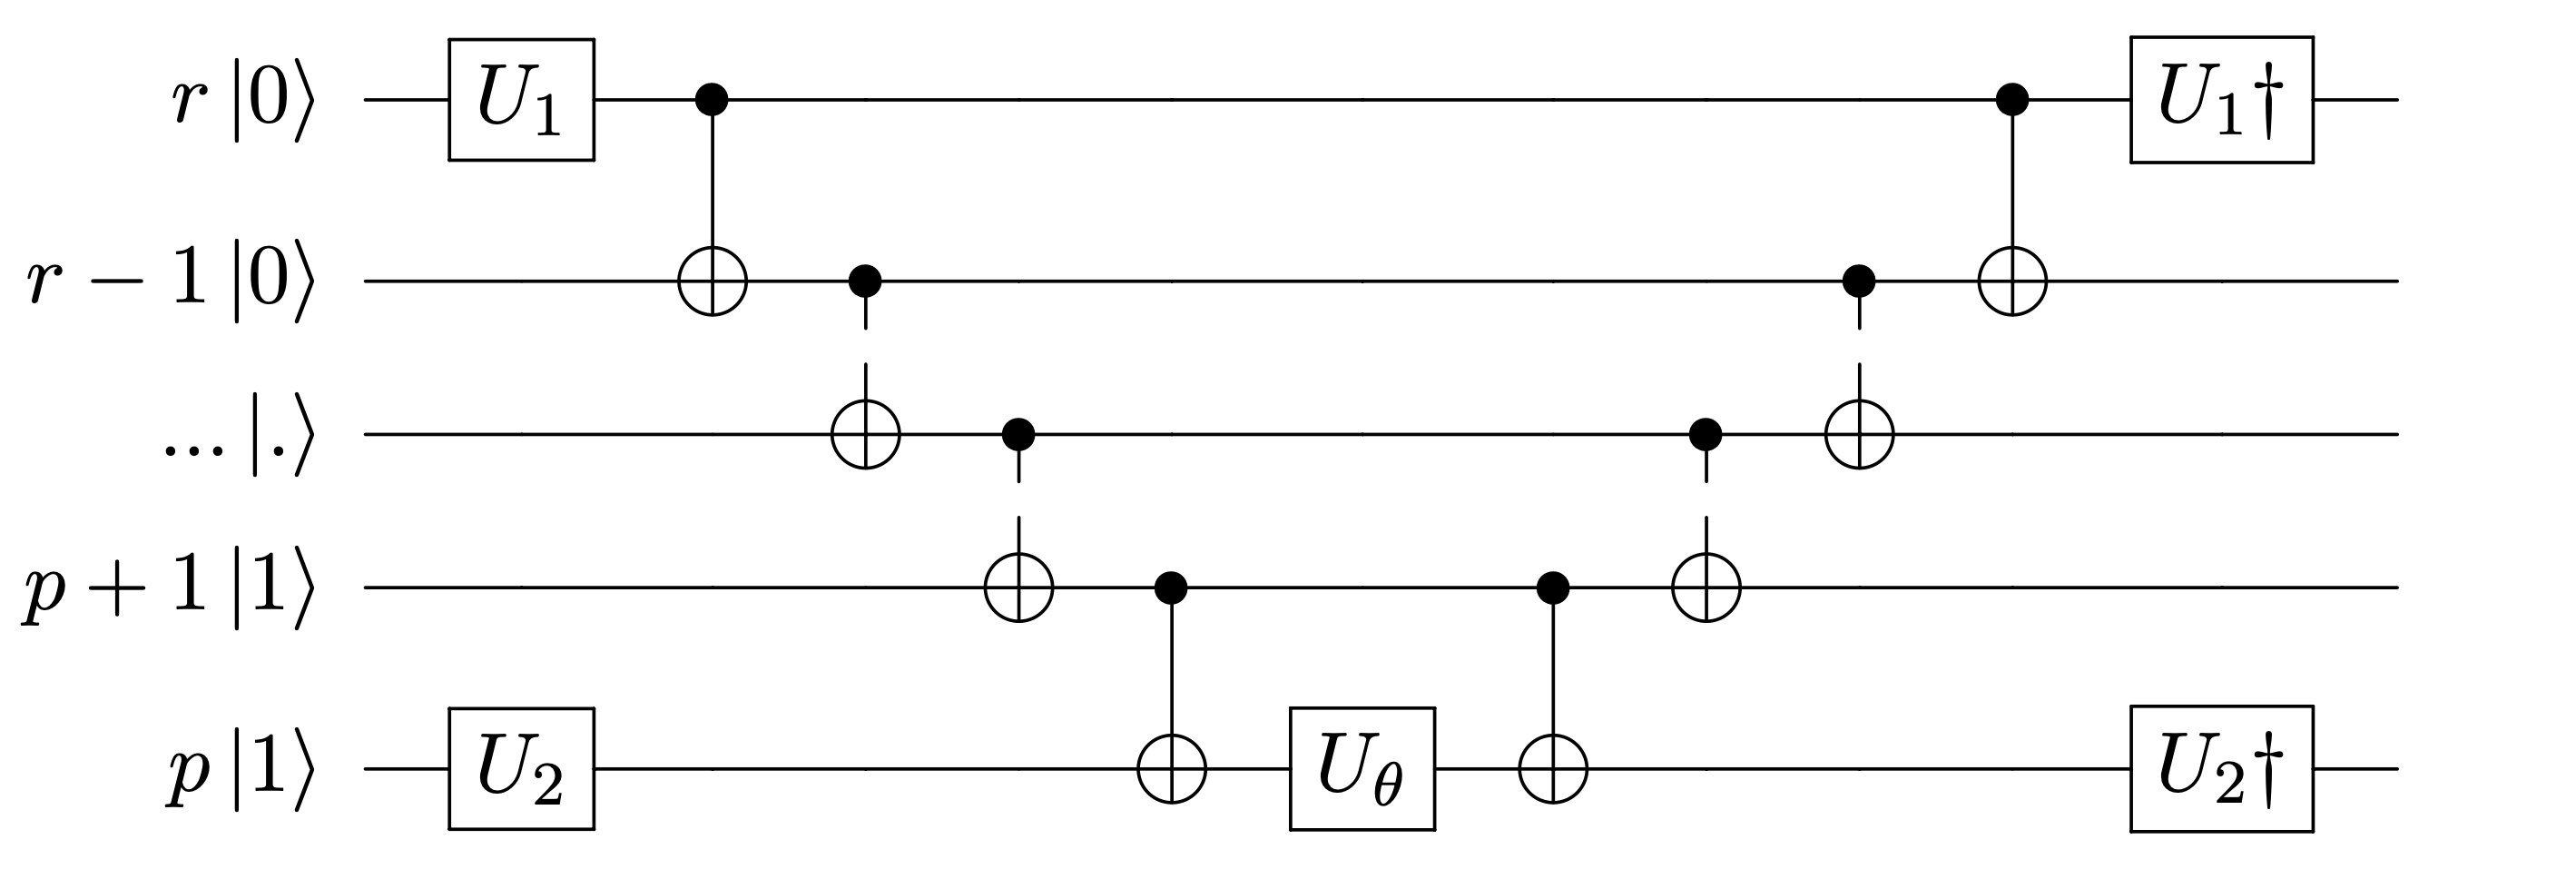
\includegraphics[width=0.8\textwidth]{Immagini/Capitolo_2/ucc_singles.png}
    \caption{Esponenziazione eccitazioni singole \cite{Carobene_2021}.}
    \label{fig:eccitazioni-singole}
\end{figure} 

con $(U_1,U_2)\in\{(Y,H),(H,Y)\}$, per l'esponenziazione di $\hat{T}_1-\hat{T}_{1}^{\dagger}$;

\begin{figure}[H]
    \centering
    \hspace{0.5cm}
    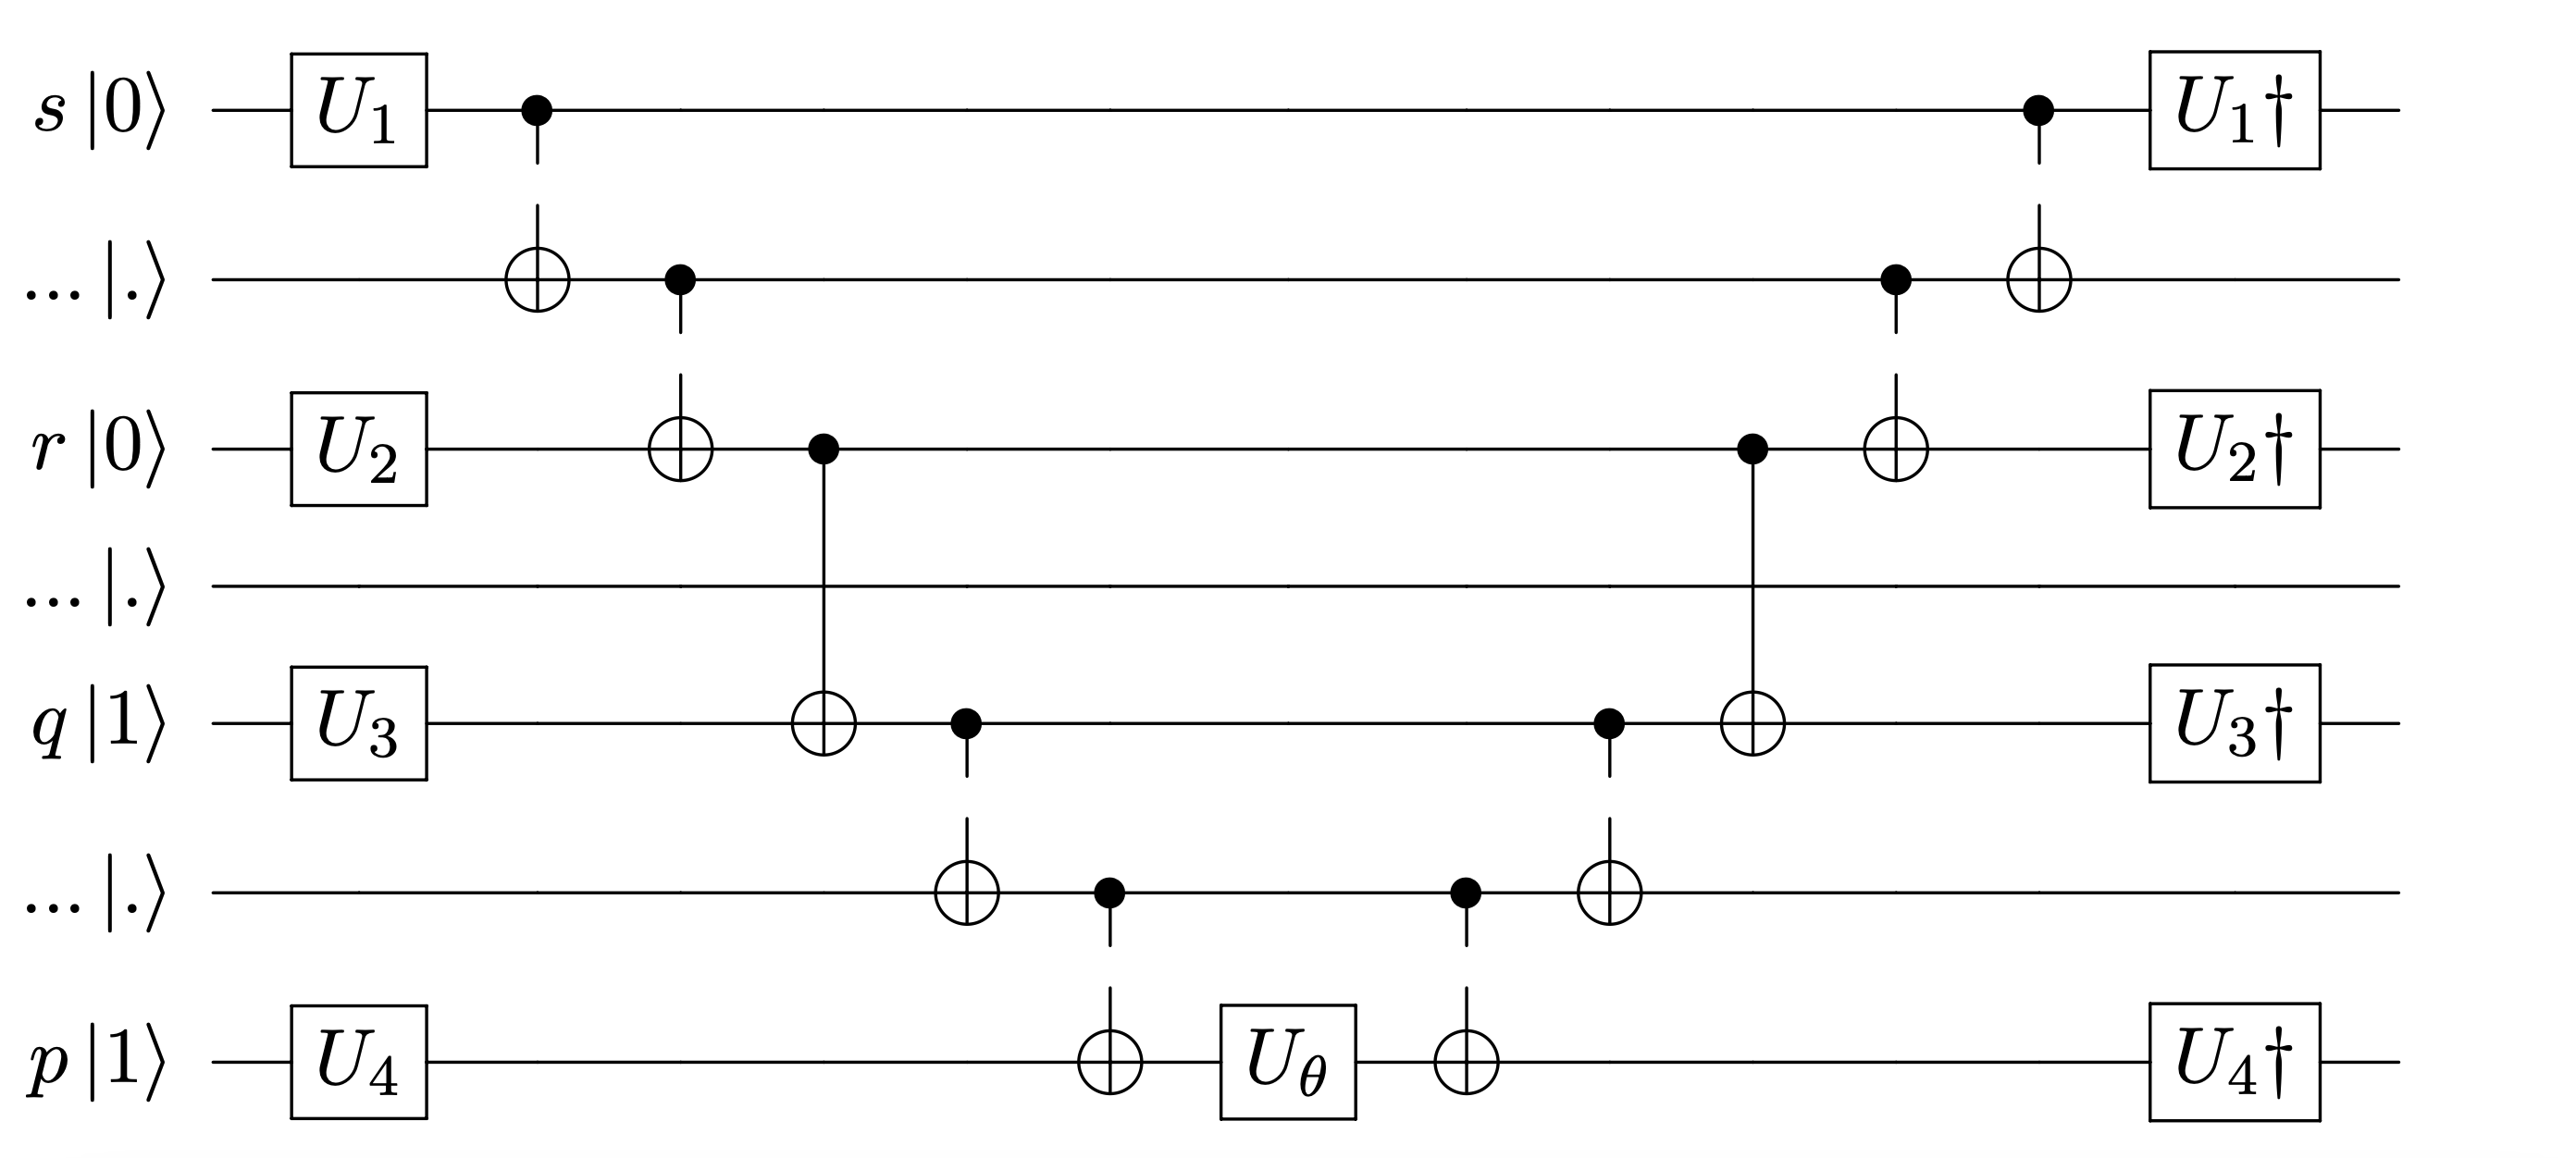
\includegraphics[width=0.8\textwidth]{Immagini/Capitolo_2/ucc_doubles.png}
    \caption{Esponenziazione eccitazioni doppie \cite{Carobene_2021}.}
    \label{fig:eccitazioni-doppie}
\end{figure} 

dove 
\begin{align*}
    (U_1,U_2,U_3,U_4)\in\{&(H,H,Y,H),(Y,H,Y,Y),(H,Y,Y,Y),(H,H,H,Y),\\
    &(Y,H,H,H),(H,Y,H,H),(Y,Y,Y,H),(Y,Y,H,Y)\}
\end{align*}

per l'esponenziazione di $\hat{T}_2-\hat{T}_{2}^{\dagger}$.

Per formare l'ansatz UCCSD basterà concatenare questi due circuiti allo stato HF di partenza.

% --------------------------------------------------------------------------------------------------------------
\subsection{Pair Unitary Coupled Cluster Doubles (pUCCD)}\label{subsec:pUCCD}

Nell'approccio pUCCD si selezionano soltanto le eccitazioni doppie e si impone che queste agiscano sempre su coppie di elettroni. Se si studia un sistema con numero pari di elettroni nello stato fondamentale e se ne considerano i $K$ orbitali spaziali, si può definire l'operatore di eccitazione doppia accoppiata:

\begin{equation}\label{eqn:operatore-paired-cluster}
    \hat{T}_{\text{pCCD}} = \sum_{a,r} 
    \theta_{a_\alpha a_\beta}^{r_\alpha r_\beta}\,
    a^{\dagger}_{a_\alpha} a^{\dagger}_{a_\beta} a_{r_\alpha} a_{r_\beta}
\end{equation}

dove $a,r$ stavolta indicizzano gli orbitali spaziali, all'interno dei quali $\alpha,\beta$ indicano lo spin. La funzione d'onda pUCCD è definita così:

\begin{equation}
    \ket{\text{pUCCD}} = e^{\hat{T}_{\text{pCCD}} - \hat{T}_{\text{pCCD}}^{\dagger}} \ket{HF}
\end{equation}

dove si è usato $\ket{HF}$ per indicare la soluzione di Hartree-Fock di riferimento. Questo appaiamento determina una sostanziale diminuzione nel numero di parametri variazionali e di gate richiesti, al prezzo di una minore capacità di rappresentare il problema in esame. Esiste tuttavia una strategia correttiva: i risultati ottenuti con pUCCD, in particolare quelli relativi all'energia di dissociazione, migliorano significativamente se corretti tramite \inglese{orbital optimization}, con cui si può compensare l'omissione dei termini di eccitazione singola. 

% ..............................................................................................................
\subsubsection{Orbital Optimized pair Unitary Coupled Cluster Doubles (oo-pUCCD)}
% FIXME
L'ottimizzazione orbitale consiste nell'applicare un'operatore di rotazione $\hat{R}=e^{-\hat{\mathcal{K}}}$, che agisce sugli orbitali di spin $\{\phi_k\}$ \cite{Sokolov_2020,Zhao_2023}

\begin{equation}\label{eqn:ansatz-oo-pUCCD}
    \ket{\text{oo-pUCCD}} = e^{-\hat{\mathcal{K}}} \ket{\text{pUCCD}}
\end{equation}

$\hat{\mathcal{K}}$ è un'operatore \textbf{anti-hermitiano} $\hat{\mathcal{K}}^\dagger = - \hat{\mathcal{K}}$, che sostanzialmente rende conto delle eccitazioni singole precedentemente trascurate \cite{Mizukami_2020}. 

\begin{equation}\label{eqn:operatore-K}
    \hat{\mathcal{K}} = \sum_{p<q} \mathcal{K}_{pq} (a_{q}^{\dagger}a_{p} - a_{p}^{\dagger}a_{q})
\end{equation}

Il valore di aspettazione diventa:

\begin{equation}\label{eqn:energia-oo-pUCCD}
    \bra{\text{pUCCD}} e^{\hat{\mathcal{K}}} \hat{H} e^{-\hat{\mathcal{K}}} \ket{\text{pUCCD}} 
\end{equation}

e in seguito alla trasformazione degli orbitali, vengono modificati gli integrali ad uno (eq. \ref{eqn:integrale-un-elettrone}) e due corpi (eq. \ref{eqn:integrale-due-elettroni}) utilizzati per generare l'hamiltoniana di seconda quantizzazione:

\begin{subequations}\label{eqn:trasformazione-integrali}
\begin{align}
    \tilde{h}_{pq}   &= \sum_{uv}\; C_{up}^{\star}\, h_{uv} \,C_{vq}\\
    \tilde{g}_{pqrs} &= \sum_{uvxy} C_{up}^{\star}C_{vq}^{\star}\, g_{uvxy} \,C_{xr}C_{ys}
\end{align}
\end{subequations}

dove si è indicato $C_{pq} = [ e^{\hat{-\mathcal{K}}} ]_{pq}$. Per determinare il set di $\{\mathcal{K}_{pq}\}$ che minimizzano l'energia (eq. \ref{eqn:energia-oo-pUCCD}) si costruisce il circuito oo-pUCCD concatenando a pUCCD l'operatore $e^{\hat{\mathcal{K}}}$, seguendo gli stessi passaggi descritti alla Sezione~\ref{sez:quantum-coupled-cluster}. 
Dunque si procede con la minimizzazione variazionale tramite VQE (sez. \ref{subsec:VQE}) ma stavolta, dopo ciascuna ottimizzazione dei parametri, vengono ricalcolati gli integrali utilizzando le relazioni~\ref{eqn:trasformazione-integrali} e l'hamiltoniana viene trasformata di conseguenza. 

% ==============================================================================================================
\section{Hardware efficient ansatzes}\label{sez:hardware-efficient}

UCC rientra nella categoria degli ansatze \inglese{problem inspired}, costruiti a partire da considerazioni sulla fisica del problema da risolvere. Funzioni d'onda di questo tipo promettono di fornire risultati soddisfacenti, ma possono risultare impossibili da implementare, nelle condizioni attuali, per applicazioni aldilà delle semplici dimostrazioni \cite{Bharti_2022}. 

L'obiettivo primario degli ansatze \inglese{hardware-efficient} (HEA) è minimizzare profondità e numero di operazioni del circuito per rispondere alle limitazioni dei dispositivi NISQ \cite{Leone_2024}. Forme variazionali di questo tipo sacrificano l'attinenza con la teoria fisica sottostante, perciò vengono dette \inglese{problem agnostic}.

% ..............................................................................................................
\subsubsection{Ansatz rotazionali \cite{qiskit_TwoLocal}}

Un esempio di forme variazionali \inglese{hardware-efficient} sono gli \textbf{ansatz rotazionali}, così chiamati perché i loro circuiti sono costituiti da operazioni di rotazione su singolo qubit, alternate ad operazioni di entanglement. 
Un semplice schema per questo ansatz si basa sulle rotazioni parametriche $R_x(\theta)$, $R_y(\theta)$ e $R_z(\theta)$, generate attraverso l'esponenziazione delle matrici $X$, $Y$ e $Z$ introdotte alla Sezione~\ref{subsec:gates}.

\begin{subequations}\label{eqn:rotazioni-parametriche}
\begin{align}
    R_x &\equiv e^{-iX\frac{\theta}{2}} = 
    \begin{pmatrix}
        \cos\frac{\theta}{2}   &-i\sin\frac{\theta}{2}\\
        -i\sin\frac{\theta}{2} &\cos\frac{\theta}{2}
    \end{pmatrix}\\
    R_y &\equiv e^{-iY\frac{\theta}{2}} = 
    \begin{pmatrix}
        \cos\frac{\theta}{2} &-\sin\frac{\theta}{2}\\
        \sin\frac{\theta}{2} &\cos\frac{\theta}{2}
    \end{pmatrix}\\
    R_z &\equiv e^{-iZ\frac{\theta}{2}} = 
    \begin{pmatrix}
        e^{-i\frac{\theta}{2}} &0\\
        0  &e^{i\frac{\theta}{2}}
    \end{pmatrix}
\end{align}
\end{subequations}

poiché queste rotazioni appartengono al gruppo delle matrici speciali unitarie di rango 2 [SU(2)] \cite{McMillan_2019}, rappresentate da matrici 2$\times$2 unitarie con determinante 1, gli ansatze rotazionali di questo tipo vengono soprannominati EfficientSU(2).  

Un esempio di circuito EfficientSU(2) su 3 qubit che impiega soltanto $R_y$ e $R_z$ potrebbe essere:

\begin{figure}[H]
\begin{center}
\begin{quantikz}
\gate{R_y(\theta_1)} & \gate{R_z(\theta_3)} & \ctrl{1} & \ctrl{2} & \qw      & \gate{R_y(\theta_6)} & \gate{R_z(\theta_9)}\\
\gate{R_y(\theta_2)} & \gate{R_z(\theta_4)} & \targ{ } & \qw      & \ctrl{1} & \gate{R_y(\theta_7)} & \gate{R_z(\theta_10)}\\
\gate{R_y(\theta_3)} & \gate{R_z(\theta_5)} & \qw      & \targ{ } & \targ{ } & \gate{R_y(\theta_8)} & \gate{R_z(\theta_11)}
\end{quantikz}
\end{center}
\caption{Esempio di ansatz rotazionale.}
\end{figure}

Per migliorare la convergenza, è possibile aumentare i parametri circuitali ripetendo questo insieme di rotazioni ed entanglement un numero $D$ arbitrario di volte, al prezzo di una maggiore profondità. 



% Capitolo 3

\chapter{Simulazioni}

Le simulazioni presentate in questo capitolo si concentrano prevalentemente sulla molecola di idruro di litio (LiH), scelta per la sua struttura di piccole dimensioni e per il numero contenuto ridotto di orbitali elettronici coinvolti, che la rendono un sistema ideale per testare metodi quantistici. In particolare, è stata calcolata l’energia dello stato fondamentale al variare della distanza internucleare, con l’obiettivo di tracciare il profilo del potenziale elettronico. In LiH, il minimo di energia si colloca attorno a $1.595$ \AA, in accordo con dati sperimentali disponibili in letteratura \cite{LiH_nist}. I dettagli relativi alle simulazioni, inclusi i codici utilizzati, sono consultabili e disponibili nella \inglese{repository} GitHub: \cite{AnsOME}.

% ==============================================================================================================
\section{Introduzione al codice}\label{sez:introduzione-codice}

In questa sezione viene descritto il codice utilizzato per le simulazioni, con particolare riferimento alla piattaforma offerta da Qiskit \cite{qiskit2024}, una delle piattaforme più diffuse per la programmazione quantistica. Qiskit fornisce strumenti avanzati per la creazione, simulazione e ottimizzazione di circuiti quantistici, fondamentali per affrontare problemi di chimica quantistica come la determinazione degli stati fondamentali e la simulazione di reazioni.

Si presenta una panoramica generale su come realizzare simulazioni tramite il Variational Quantum Eigensolver (VQE) in Qiskit, illustrando i passaggi essenziali e le scelte metodologiche chiave. Inoltre, vengono approfonditi alcuni concetti specifici, come la scelta delle basi e degli ottimizzatori, elementi centrali nella configurazione delle simulazioni quantistiche.
La selezione della base influenza direttamente la rappresentazione della molecola, determinando sia il numero di qubit richiesti che l’accuratezza dei risultati. Basi meno complesse, come la STO-3G, vengono spesso utilizzate per ridurre il costo computazionale, mentre basi più articolate, come la 6-31G, possono migliorare la precisione dei risultati a scapito di una maggiore complessità.
Gli ottimizzatori, d’altra parte, influenzano il processo di minimizzazione dell’energia e la velocità con cui si raggiunge la convergenza. A seconda del problema e delle caratteristiche della simulazione, è possibile scegliere tra diversi \inglese{optimizers} presto implementabili con Qiskit, come SPSA, COBYLA e SLSQP, ciascuno con vantaggi specifici per scenari diversi.


% --------------------------------------------------------------------------------------------------------------
\subsection{Impostazione del problema}

Il primo passo è implementare il sistema molecolare all'interno del codice attraverso \myinline{PySCFDriver}, che fa da ponte fra le classi di Qiskit e la libreria di chimica PySCF~\cite{pyscf}. Come argomenti si inseriscono gli attributi della molecola, quindi si esegue il metodo \myinline{.run()} per estrarre un \myinline{ElectronicStructureProblem}: oggetto che rappresenta il problema elettronico. 

% DRIVER ________________________________________________________
\begin{tcolorbox}[title=Dichiarazione molecola]
\begin{lstlisting}[language=Python]
LiH_geometry = f"""Li 0. 0. 0.; H 0. 0. {distance}"""

driver = PySCFDriver(
           atom   = LiH_geometry,
           basis  = 'sto3g',
           charge = 0,
           spin   = 0,
           unit   = DistanceUnit.ANGSTROM
         )

problem = driver.run()
\end{lstlisting}
\vspace{-0.2cm}
\end{tcolorbox}

Con \myinline{FreezeCoreTransformer} si possono congelare gli orbitali \inglese{core} della molecola, il che permette di ridurre la dimensione del problema con una piccola perdita di precisione dovuta all'approssimazione. Questo compromesso è generalmente considerato ragionevole, poiché il contributo degli orbitali esclusi diventa un semplice shift all'energia totale.

% PROBLEM _______________________________________________________
\begin{tcolorbox}[title=Congelamento orbitali core e hamiltoniana]
\begin{lstlisting}
fc_transformer = FreezeCoreTransformer()
fc_problem     = fc_transformer.transform(problem)
\end{lstlisting}
\vspace{-0.2cm}
\end{tcolorbox}

% ..............................................................................................................
\subsubsection{Scelta della base}

Ad oggi sono state introdotte numerose basi per rappresentare gli orbitali molecolari, alcune delle quali permettono di ottenere accuratezze elevate, anche se il costo computazionale cresce rapidamente all’aumentare del numero di orbitali atomici. Le basi STO-$n$G vengono principalmente impiegate per studi preliminari e approssimativi, mentre calcoli più dettagliati richiedono basi più articolate. Un esempio di queste è 6-31G, una base di tipo \inglese{split-valence} che combina sei funzioni gaussiane per il \inglese{core} e due serie di gaussiane per gli elettroni di valenza, migliorando la descrizione degli orbitali.

Di seguito è riportato il Grafico~\ref{fig:FCI-e-basi}, in cui si confrontano i risultati di FCI nelle basi STO-3G, STO-6G e 6-31G. 

\begin{figure}[H]
    \centering
    \hspace{-1cm}
    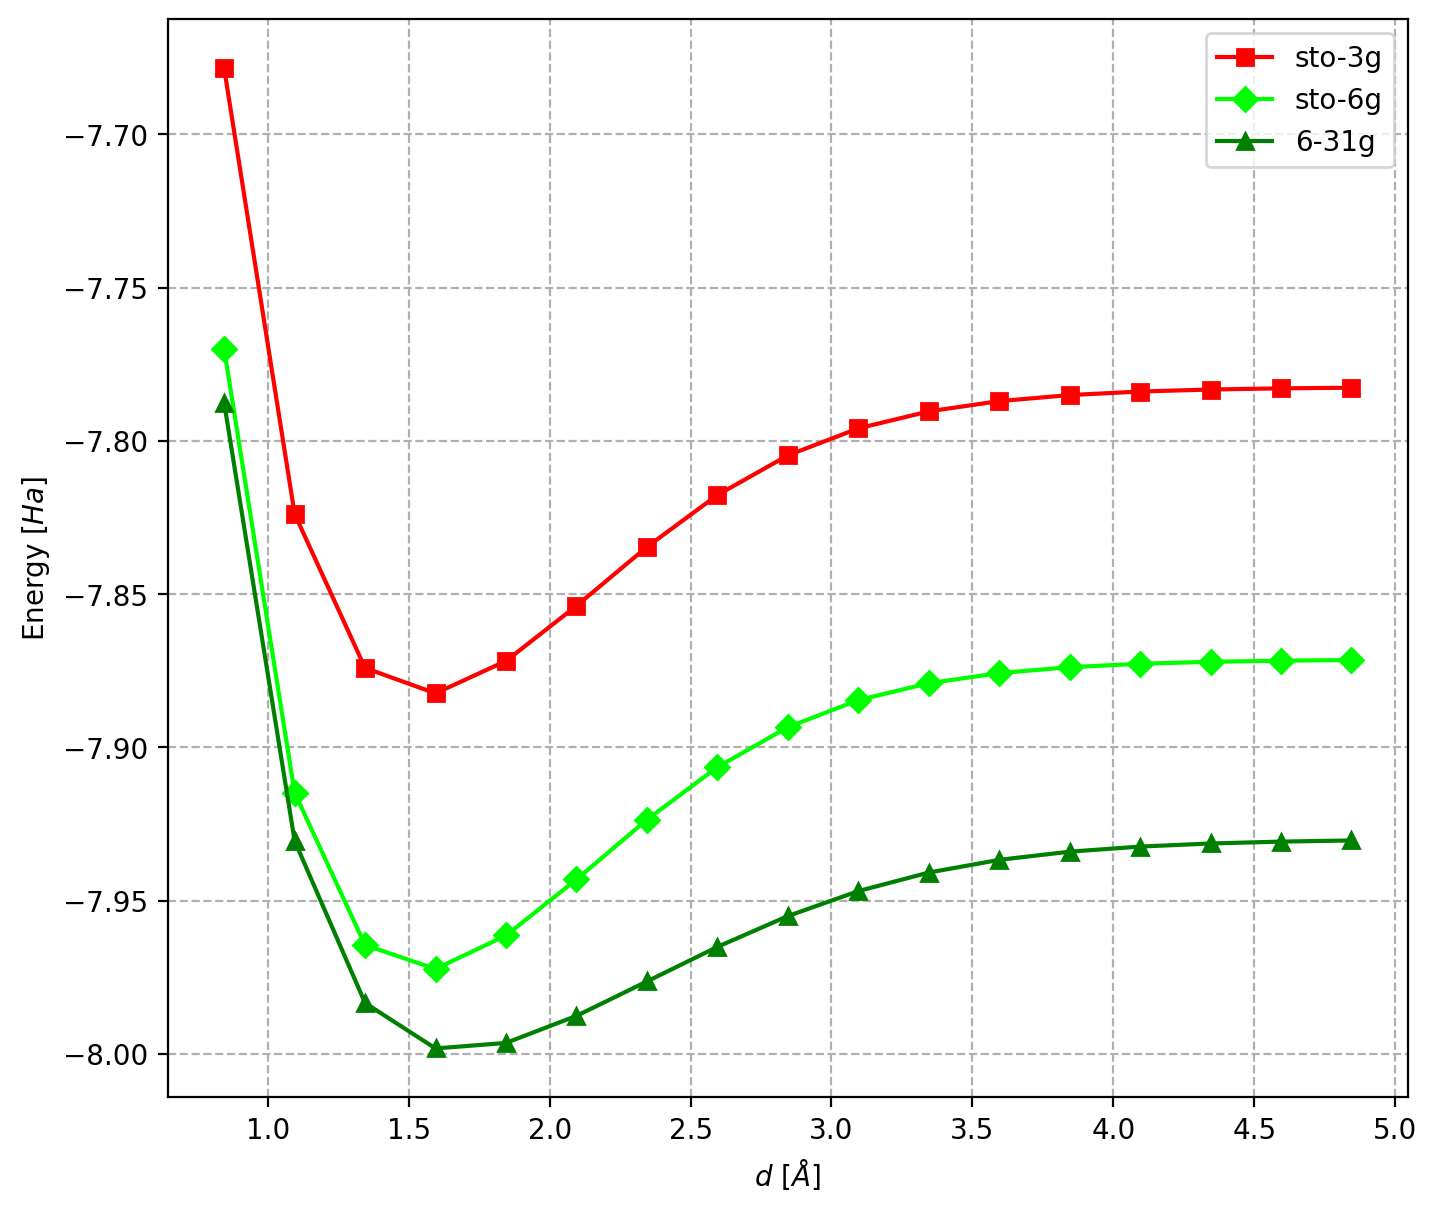
\includegraphics[width=.6\linewidth]{Immagini/Capitolo_3/FCI_e_basi.png}
    \caption{LiH: FCI con diverse basi.}
    \label{fig:FCI-e-basi}
\end{figure}

Le STO-$n$G sovrastimano l’energia in modo marcato ma richiedono tempi di calcolo notevolmente inferiori rispetto a 6-31G. In questo lavoro l’obiettivo è confrontare il costo di diversi circuiti quantistici, per cui è sufficiente lavorare con la base STO-3G.

\newpage

% --------------------------------------------------------------------------------------------------------------
\subsection{Ansatz}

\begin{minipage}{0.58\textwidth}
    Qiskit offre un'ampia scelta di ansatze UCC \cite{qiskit_UCC}, implementabili con poche righe di codice, qui sotto esemplificate per un generico ordine di eccitazioni~$X$. Si veda ad esempio il circuito $q$-UCCS, riportato qui a destra, generato dalla classe \myinline{UCCS} per le analisi della molecola di LiH. Innanzitutto, si può notare che la base STO-3G utilizzata per definire il problema dà luogo ad un circuito con 10 qubit, che per motivi di lunghezza viene suddiviso in quattro sezioni. 
    Come illustrato in Sezione~\ref{subsec:coupled-cluster}, la funzione d'onda \inglese{Coupled Cluster} è costruita a partire da uno stato di Hartree-Fock; i qubit 0 e 5, a cui vengono applicate delle rotazioni U, corrispondono agli stati occupati, mentre gli altri rappresentano orbitali \textbf{virtuali}. Dopodiché, si può osservare che i gate successivi sono applicati seguendo il \inglese{pattern} presentato in Figura~\ref{fig:eccitazioni-singole}, che mostrava l'insieme di operazioni necessarie per riprodurre le eccitazioni singole.
    È importante sottolineare che, tra i circuiti $q$-UCC utilizzati, $q$-UCCS è il meno costoso in termini di risorse, con $q$-UCCD e $q$-UCCSD che possono arrivare a profondità trenta volte maggiori. 
    

\end{minipage}
\begin{minipage}{0.42\textwidth}
    \begin{figure}[H]
        \centering
        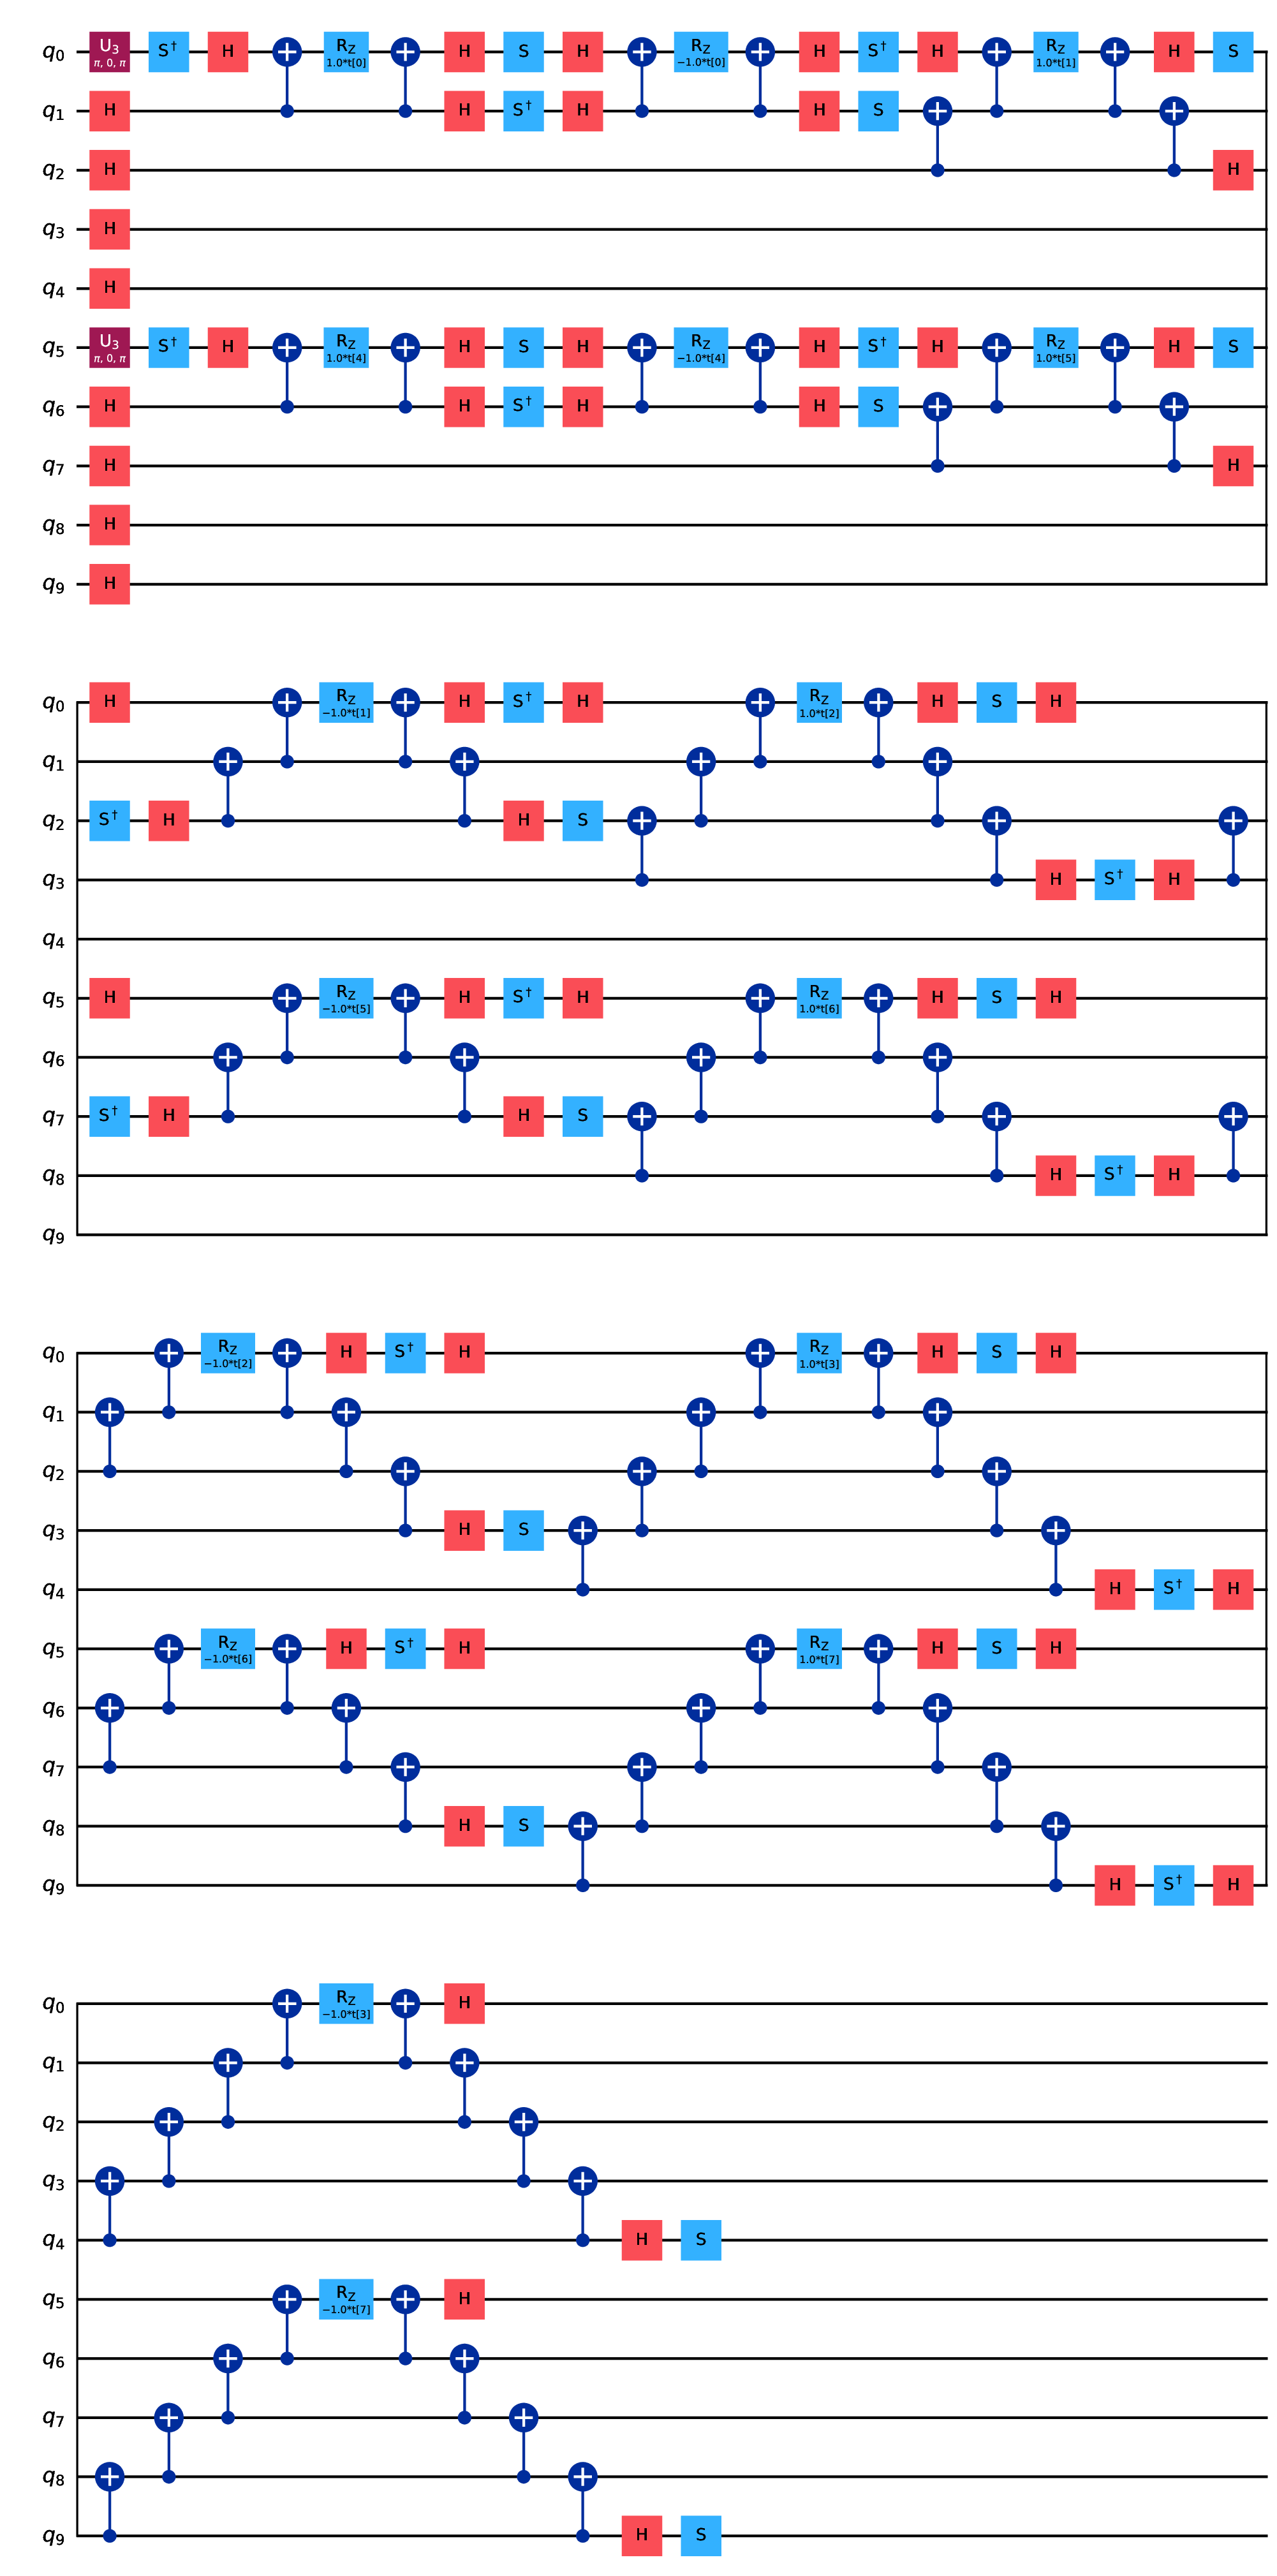
\includegraphics[width=\textwidth]{Immagini/Capitolo_3/uccs_circuit.png}
        \caption{Circuito UCCS.}
        \label{fig:circuito-uccs}
    \end{figure}
\end{minipage}

% ANSATZ UCC ____________________________________________________
\begin{tcolorbox}[title=Dichiarazione generico ansatz UCC$X$]
\begin{lstlisting}
uccx_qc = UCCX (
    fc_problem.num_spatial_orbitals,
    fc_problem.num_particles,
    mapper,
    excitations = 'x' # e.g.: 's', 'd', 'sd'
    initial_state=HartreeFock(
        fc_problem.num_spatial_orbitals,
        fc_problem.num_particles,
        mapper,
    ),
)

bounds = [[-np.pi,np.pi] for _ in range(uccx_qc.num_parameters)]
uccx_qc.parameter_bounds = bounds
\end{lstlisting}
\vspace{-0.2cm}
\end{tcolorbox}

Si noti che è necessario esplicitare un oggetto \myinline{mapper}, cioè il metodo di codifica da utilizzare per tradurre il problema in un circuito. Come discusso alla Sezione~\ref{subsec:qubit-mapping}, nelle simulazioni di questo elaborato si è utilizzato l'isomorfismo di Jordan-Wigner, espresso in Qiskit con la classe \myinline{JordanWignerMapper}.

L'ansatz rotazionale \inglese{hardware-efficient} invece viene implementato tramite la classe \myinline{EfficientSU2}, che può essere configurata con molta flessibilità:

% ANSATZ Efficient ______________________________________________
\begin{tcolorbox}[title=Dichiarazione ansatz hardware-efficient]
\begin{lstlisting}
efficient = EfficientSU2 (
    num_qubits, 
    reps=1,
    entanglement ='reverse_linear', 
    su2_gates=['ry', 'rz']
    initial_state=HartreeFock(
        fc_problem.num_spatial_orbitals,
        fc_problem.num_particles,
        mapper,
    ),
)

# stampo il circuito
efficient.draw('mpl')
\end{lstlisting}
\vspace{-0.5cm}
\begin{center}
    \hspace{-0.5cm}
    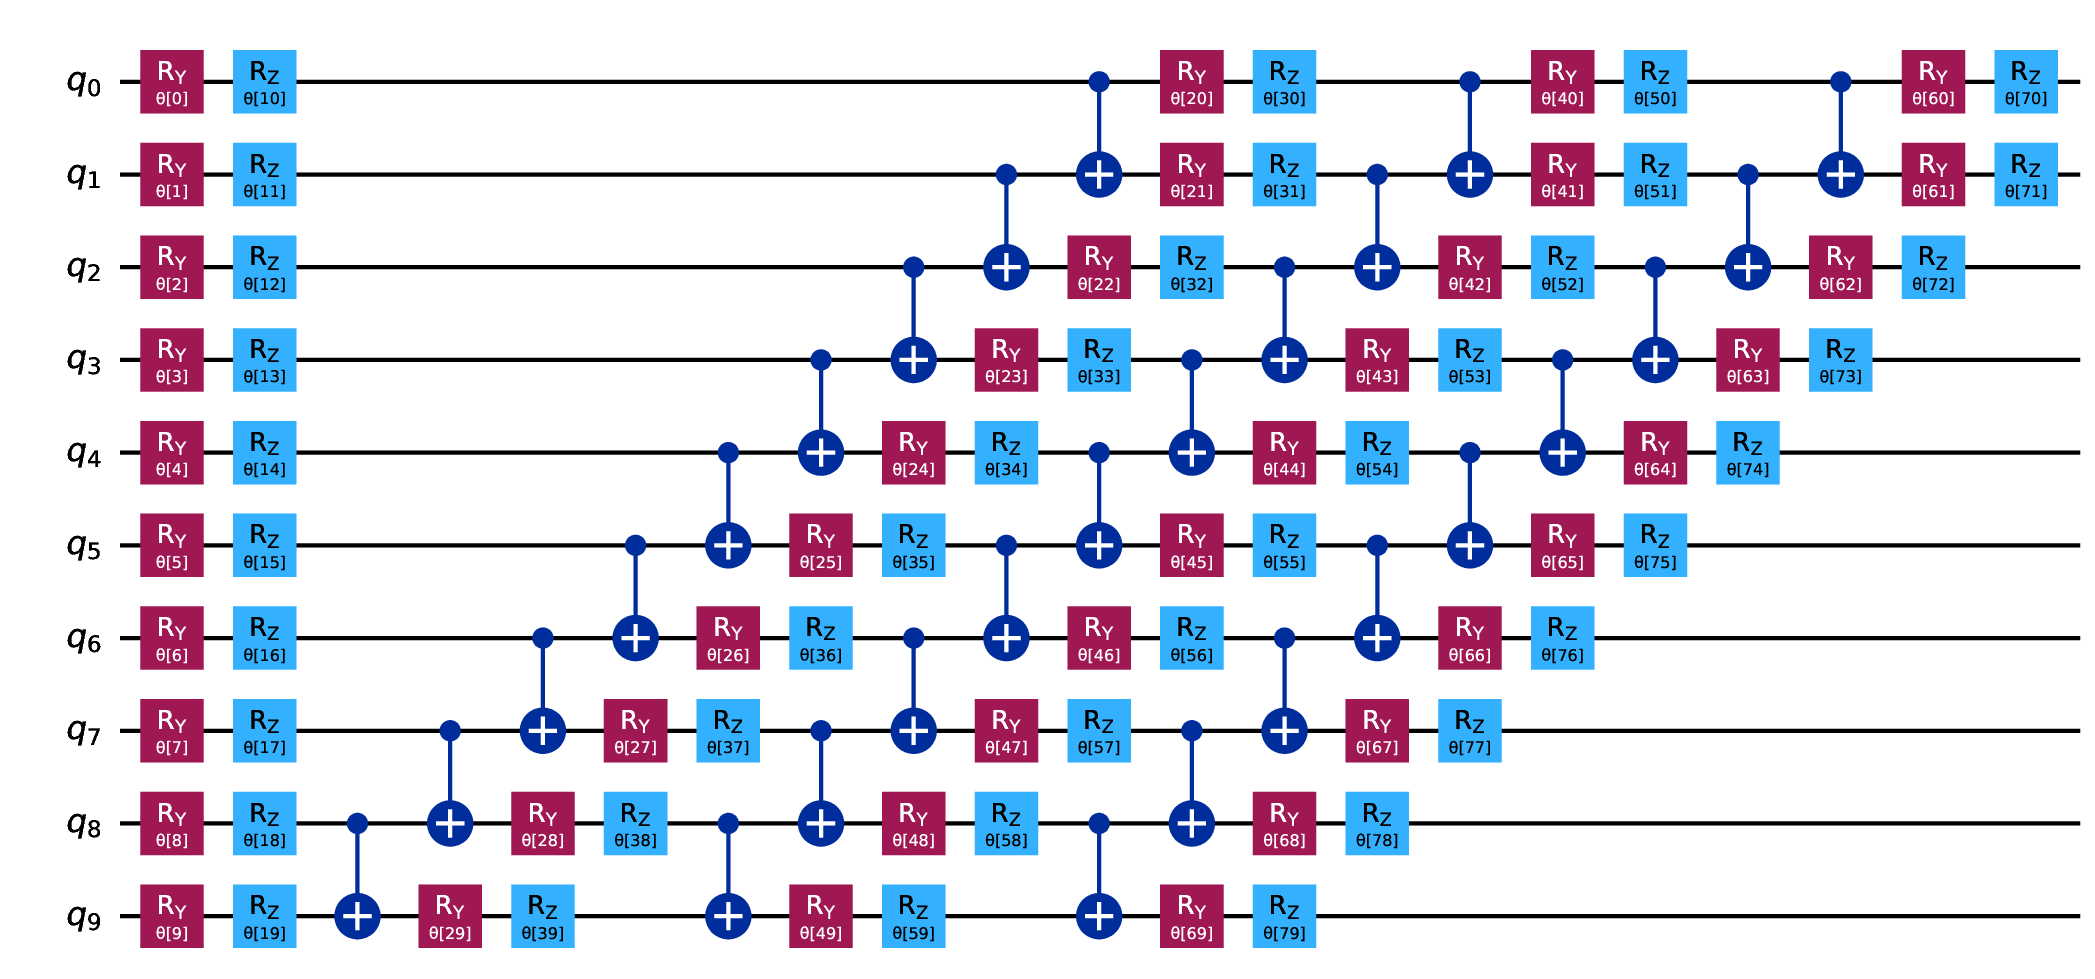
\includegraphics[width=\textwidth]{Immagini/Capitolo_3/efficient_circuit.png}
    \captionof{figure}{Circuito EfficientSU(2).}
    \label{fig:efficient-circuit}
\end{center}
\end{tcolorbox}

in cui si sono fornite le seguenti istruzioni:

\begin{itemize}
\item \myinline{reps} specifica il numero di ripetizioni del layer di rotazioni e CNOT;
\item \myinline{entanglement} specifica la struttura e l'ordine con cui vengono applicati i CNOT;
\item \myinline{su2_gates} permette di scegliere quali rotazioni applicare a ciascun qubit all'interno di un layer.
\end{itemize}

\myinline{num_qubits} dovrà necessariamente corrispondere al numero di qubit dell'operatore da valutare che, nel caso in esame, è 10.


% --------------------------------------------------------------------------------------------------------------
\subsection{VQE}

Dichiarati il problema e la forma variazionale, si passa all'implementazione degli algoritmi di calcolo, con cui si effettuano le previsioni dei valori di energia. Come introdotto in Sezione~\ref{subsec:VQE}, gli ingredienti principali di VQE sono tre: una funzione costo, una forma variazionale e un ottimizzatore. Nelle seguenti linee di codice si va proprio a dichiarare un oggetto \myinline{VQE} inserendovi l'ansatz e l'\inglese{optimizer}, insieme ad un \myinline{Estimator}, classe di Qiskit che si occupa di valutare il valore di aspettazione di un'hamiltoniana.

% VQE ___________________________________________________________
\begin{tcolorbox}[title=Implementazione VQE]
\begin{lstlisting}
vqe_solver = VQE(Estimator(), ansatz, opt)

if ini is None:
    ini = [0.0] * ansatz.num_parameters
else:
    vqe_solver.initial_point = ini

calc = GroundStateEigensolver(mapper, vqe_solver)

result = calc.solve(problem)
\end{lstlisting}
\vspace{-0.2cm}
\end{tcolorbox}

Il metodo \myinline{.solve()} di \myinline{GroundStateEigensolver} si occupa di estrarre l'hamiltoniana di seconda quantizzazione del problema elettronico, quindi la dà in pasto a VQE per calcolarne il valore di aspettazione. Infine, si possono estrarre i risultati del calcolo, raccolti negli attributi dell'oggetto \myinline{result}:

% result ________________________________________________________
\begin{tcolorbox}[title=Estrazione risultati]
\begin{lstlisting}
shift = result.extracted_transformer_energies.get("FreezeCoreTransformer", 0)
total_energy = result.groundenergy + result.nuclear_repulsion_energy + shift
\end{lstlisting}
\vspace{-0.2cm}
\end{tcolorbox}

% ..............................................................................................................
\subsubsection{Scelta dell'ottimizzatore}

VQE è un metodo ibrido, che sfrutta un \inglese{optimizer} classico per trovare i migliori parametri per la relativa forma variazionale. Tra questi, quelli più impiegati nel presente lavoro sono COBYLA \cite{powell_2007} e SLSQP \cite{kraft_1988}, ma si è voluto fare un paragone con un terzo ottimizzatore utilizzato diffusamente in letteratura: SPSA \cite{spsa_site}.

\begin{itemize}
    \item {SPSA} (Simultaneous Perturbation Stochastic Approximation): è un metodo stocastico che approssima le derivate perturbando casualmente i parametri. È progettato per essere robusto in presenza di rumore, risultando efficace su hardware reale dove gli errori sono frequenti, ma può avere prestazioni inferiori in simulazioni ideali prive di rumore.
    \item {COBYLA} (Constrained Optimization BY Linear Approximations): un metodo iterativo che ottimizza approssimando linearmente la funzione obiettivo, permettendo anche di impostare vincoli sui parametri. È utile per ottimizzazioni che richiedono stabilità e precisione in assenza di rumore.
    \item {SLSQP} (Sequential Least SQuares Programming): un metodo di ottimizzazione che utilizza le informazioni derivabili dalla funzione per individuare il minimo locale in modo accurato, con buone performance nelle simulazioni ideali.
\end{itemize}

Di seguito è riportato il Grafico~\ref{fig:LiH-ottimizzatori}, in cui si confrontano i valori calcolati dai tre ottimizzatori su ansatz $q$-pUCCD.

\begin{figure}[H]
    \centering
    \hspace{-1cm}
    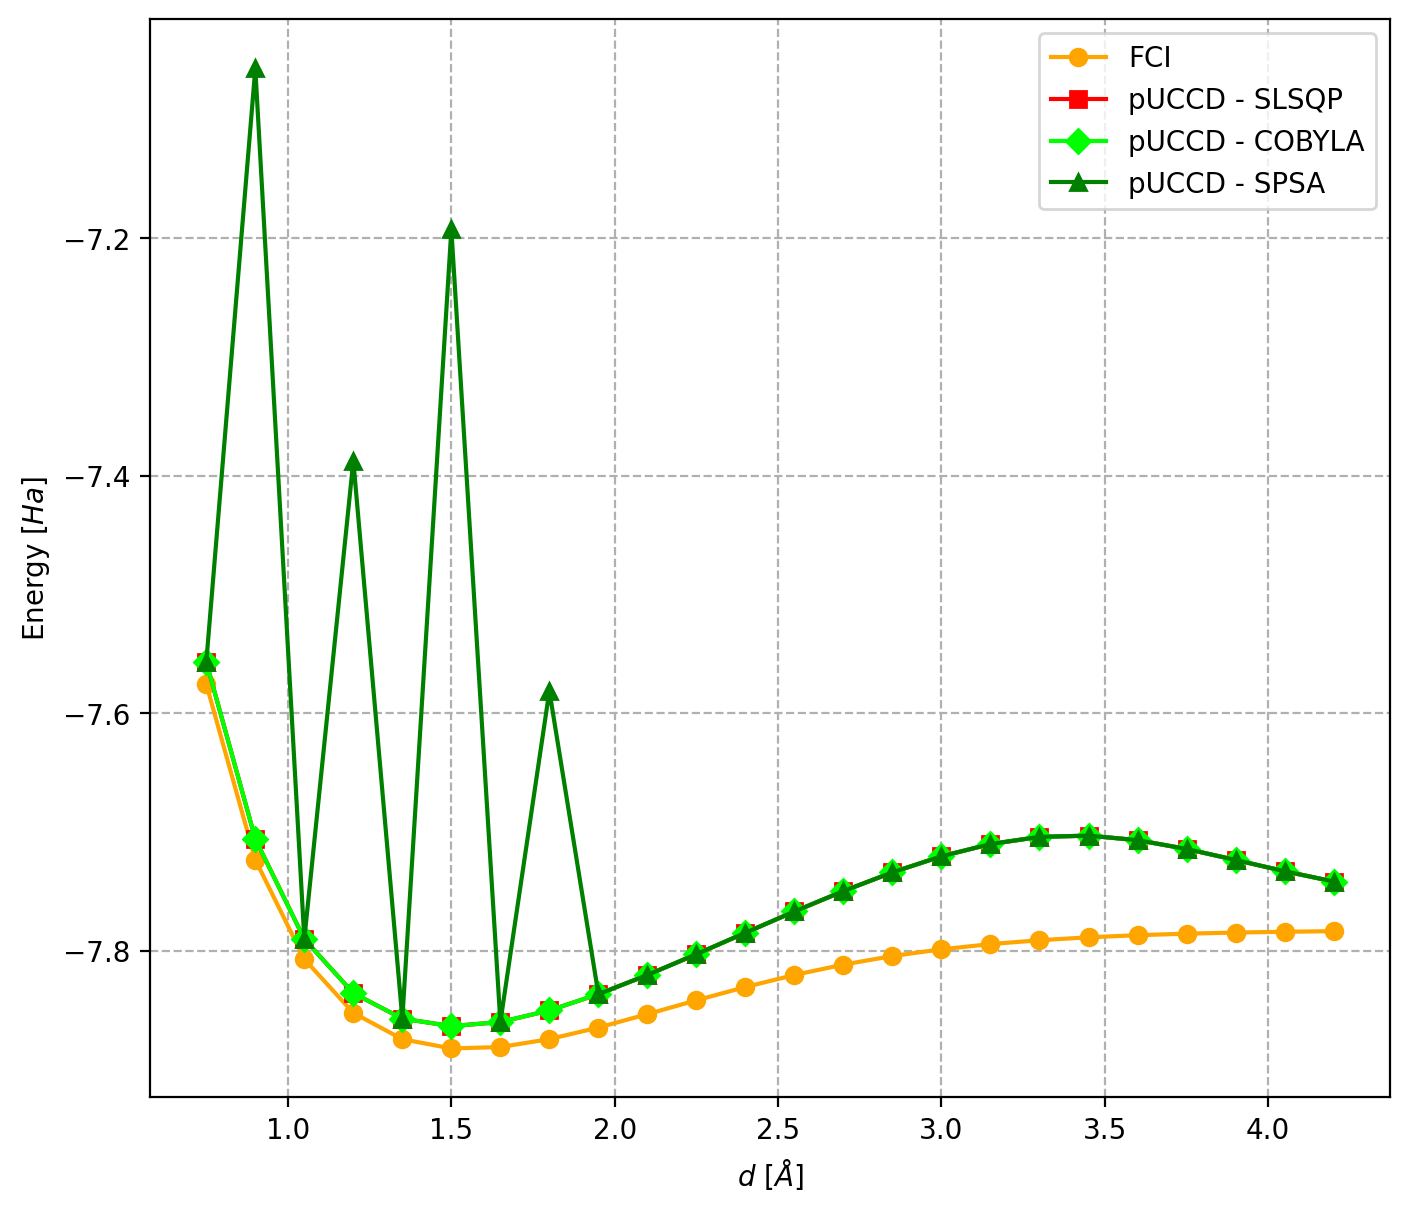
\includegraphics[width=.6\linewidth]{Immagini/Capitolo_3/LiH_optimizers.png}
    \caption{LiH: $q$-pUCCD con diversi ottimizzatori.}
    \label{fig:LiH-ottimizzatori}
\end{figure}

	
COBYLA e SLSQP convergono a risultati simili nelle energie calcolate, mentre SPSA, a parità di iterazioni, non riesce a raggiungere la convergenza. Questo può dipendere dal fatto che SPSA è ottimizzato per lavorare in condizioni rumorose, dove fornisce maggiore stabilità.







% ==============================================================================================================
\section{Confronto tra ansatze per il calcolo dell’energia}\label{sez:contronti-UCC}

In questa sezione vengono confrontate le prestazioni di vari ansatz per il calcolo dell’energia dello stato fondamentale della molecola di LiH a diversi valori della distanza internucleare. Gli ansatz analizzati comprendono diverse varianti di $q$-UCC, tra cui $q$-UCCS, $q$-UCCD, $q$-UCCSD, e $q$-pUCCD, oltre a EfficientSU(2), di tipo \inglese{hardware-efficient}. L’obiettivo è valutare le differenze di prestazioni in termini sia di accuratezza energetica sia di complessità circuitale. I calcoli sono stati eseguiti su simulatori ideali, quindi senza rumore hardware, ma possono comunque offrire un’indicazione del potenziale di ciascun metodo per applicazioni pratiche.

Coerentemente con quanto esposto nelle Sezioni~\ref{sez:quantum-coupled-cluster} e \ref{sez:hardware-efficient}, ci si attende di osservare prestazioni migliori in quegli ansatz che considerano un maggior numero di configurazioni: $q$-UCCSD e $q$-UCCD.  Tuttavia, se da un lato è chiaro che $q$-UCCSD raggiunga il risultato più accurato, lo stesso non si può dire per le soluzioni intermedie: sarà rilevante osservare fino a che punto possano competere in precisione le alternative meno costose, come $q$-pUCCD e EfficientSU(2). Ques'ultimo, in particolare, dovrebbe risultare l’ansatz meno costoso - fra quelli analizzati~- in termini di operazioni richieste. Per quanto riguarda $q$-UCCS, ci si aspetta una \inglese{performance} più debole, dal momento che le eccitazioni singole includono un basso numero di configurazioni.

La Figura~\ref{fig:LiH-confronti} riporta il confronto tra i valori energetici calcolati per ciascun ansatz. Per contestualizzare il miglioramento ottenuto grazie alla considerazione della correlazione elettronica (sez. \ref{sez:post-HF}), viene inclusa anche l’energia ottenuta con il metodo di Hartree-Fock (sez. \ref{subsec:Hartree-Fock}). Al di sotto, la Tabella~\ref{tab:energie-e-circuiti} riporta i valori dell’energia per ciascun ansatz alle distanze di legame ($E_0$) e a lungo raggio ($E_\infty$), oltre che la massima deviazione riscontrata dal valore FCI, $\Delta E_{\text{max}}$, fornendo una visione d'insieme sulle differenze tra gli approcci sia in termini di accuratezza che di complessità del circuito.

\begin{figure}[H]
    \centering
    \hspace{-0.9cm}
    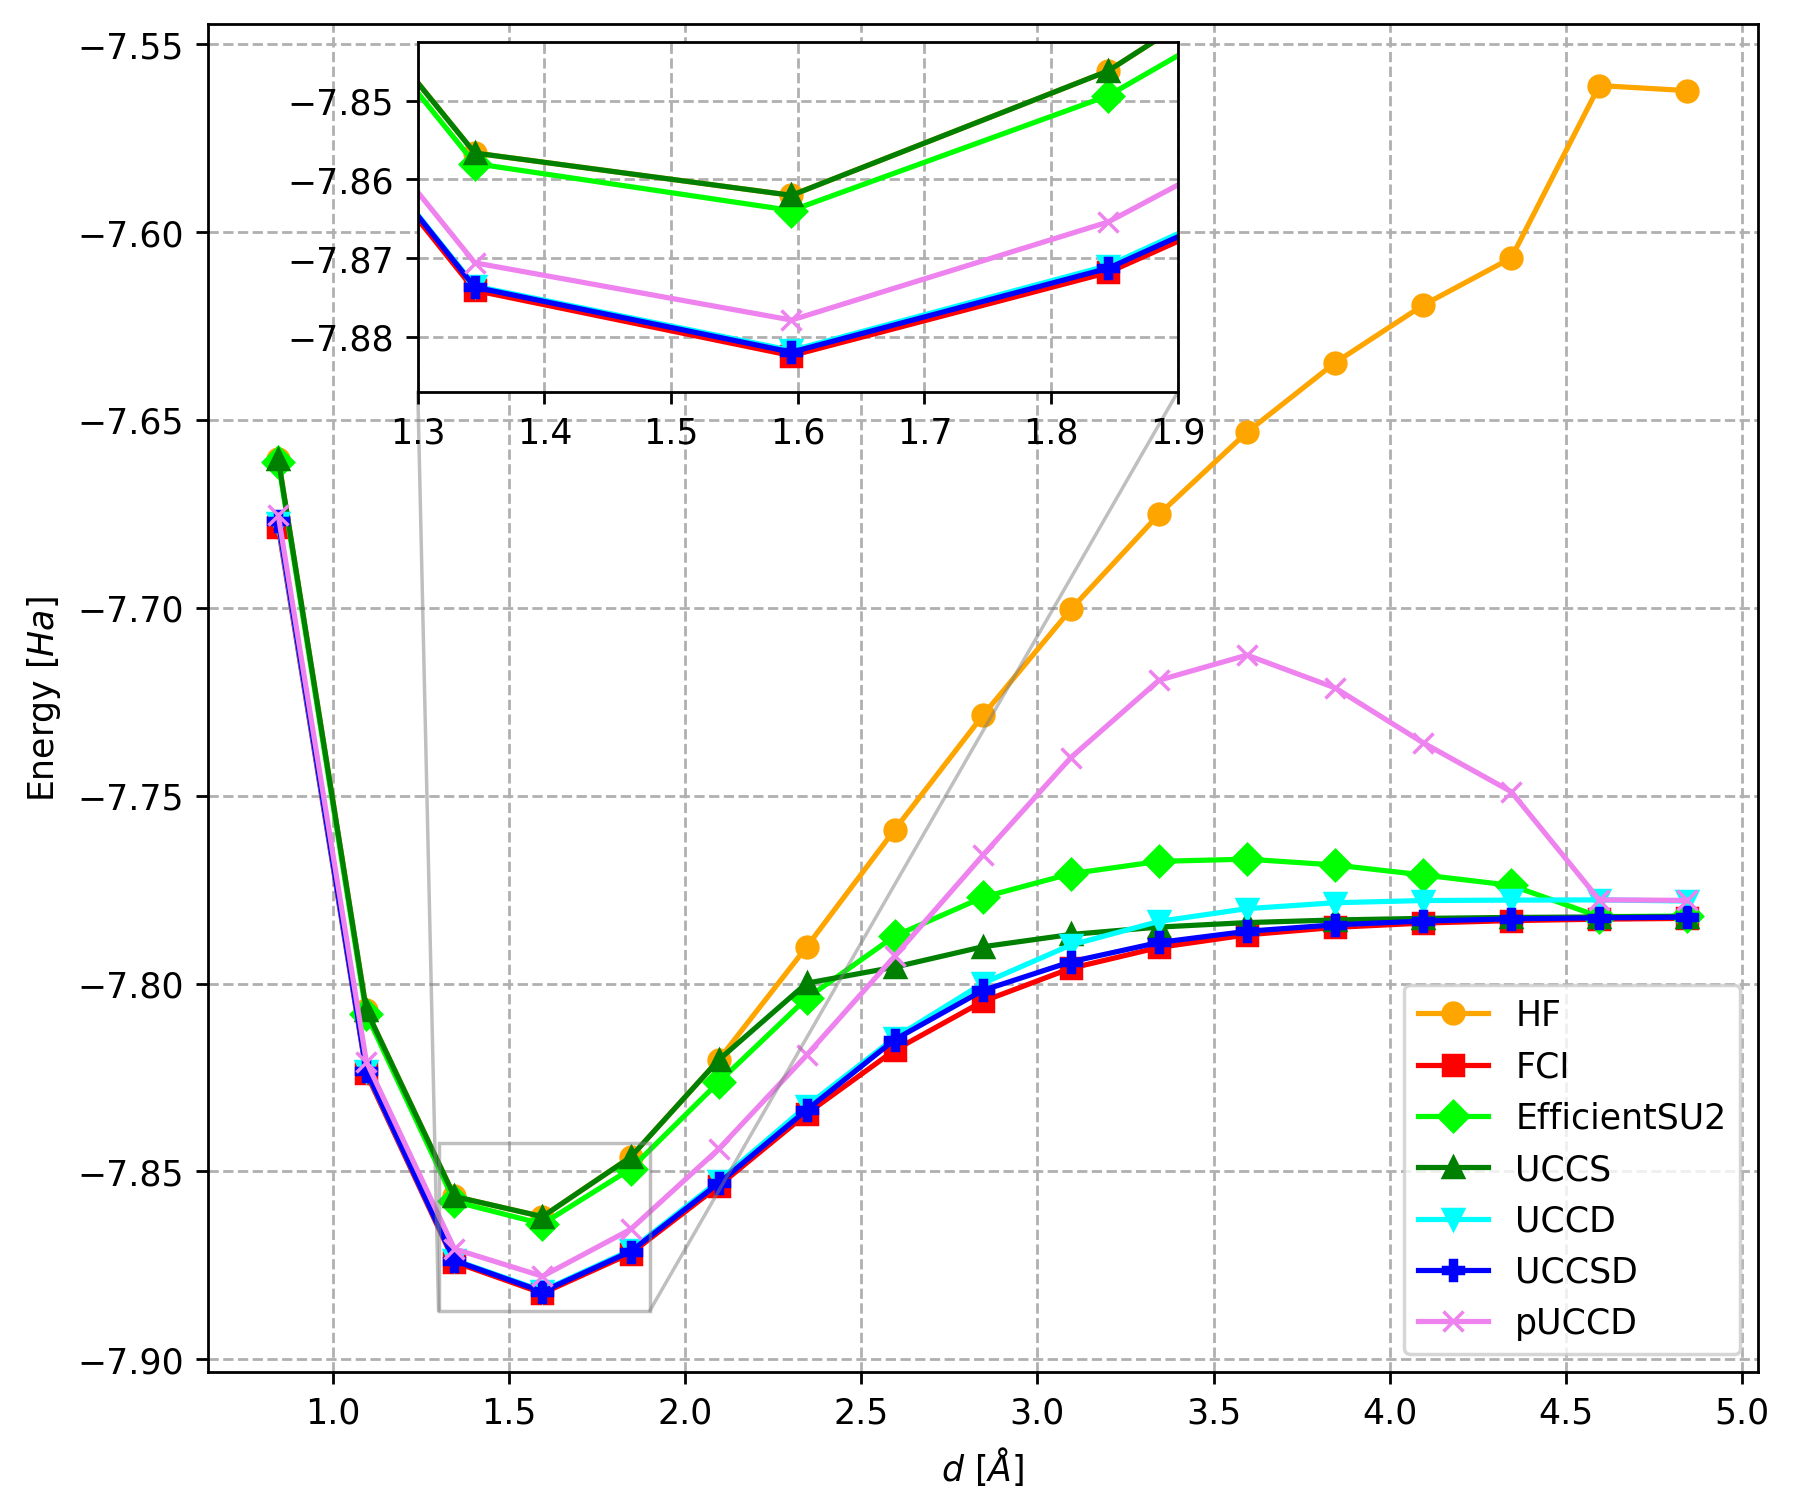
\includegraphics[width=.6\linewidth]{Immagini/Capitolo_3/LiH_ground.png}
    \caption{LiH: confronto tra ansatze.}
    \label{fig:LiH-confronti}
\end{figure}

% Please add the following required packages to your document preamble:
% \usepackage[table,xcdraw]{xcolor}
% Beamer presentation requires \usepackage{colortbl} instead of \usepackage[table,xcdraw]{xcolor}
% Please add the following required packages to your document preamble:
% \usepackage[table,xcdraw]{xcolor}
% Beamer presentation requires \usepackage{colortbl} instead of \usepackage[table,xcdraw]{xcolor}
\begin{table}[H]
    \centering
    \begin{tabular}{|c|c|c|c|c|c|c|}
    \hline
    \textbf{Metodo}                                                 & \textbf{Depth} & \textbf{CNOT} & \textbf{Parametri} & \textbf{$E_0$} & \textbf{$E_\infty$} & \textbf{$\Delta E_{\text{max}}$} \\ \hline
    \textbf{\color[HTML]{CB0000} FCI}          & /              & /             & /                  & -7.8824             & -7.7827                  & /                                     \\ \hline
    \textbf{\color[HTML]{32CB00} EfficientSU2} & 21             & 40            & 80                 & -7.8640             & -7.7820                  & 0.03                                  \\ \hline
    \textbf{\color[HTML]{036400} $q$-UCCS}     & 71             & 80            & 8                  & -7.8620             & -7.7820                  & 0.04                                  \\ \hline
    \textbf{\color[HTML]{34CDF9} $q$-UCCD}     & 2032           & 1536          & 16                 & -7.8817             & -7.7780                  & 0.007                                 \\ \hline
    \textbf{\color[HTML]{3531FF} $q$-UCCSD}    & 2098           & 1616          & 24                 & -7.8820             & -7.7823                  & 0.003                                 \\ \hline
    \textbf{\color[HTML]{D952D8} $q$-pUCCD}    & 511            & 384           & 4                  & -7.8779             & -7.7779                  & 0.07                                  \\ \hline     
\end{tabular}
\caption{Energie calcolate in hartree (Ha) e dimensioni dei circuiti.}
\label{tab:energie-e-circuiti}
\end{table}

Prima di tutto, si può notare che le previsioni HF si discostano molto dal valore di FCI, specialmente a grandi distanze. È quindi evidente che, per quanto semplice, l'approssimazione di Hartree-Fock non restituisce valori sufficientemente accurati.
Gli ansatze $q$-UCCSD, praticamente sovrapposto a FCI, e $q$-UCCD si confermano i metodi \inglese{} più precisi, con il primo che mostra una distanza massima in energia dal valore di riferimento di soli 0.003 hartree, e il secondo che si mantiene nello stesso ordine di grandezza con 0.007 Ha. La deviazione di $q$-UCCS invece è paragonabile a quella di EfficientSU(2), entrambe quasi dieci volte maggiori dei circuiti precedenti. Tuttavia, è interessante notare che, sempre in termini di deviazione massima, l'ansatz \inglese{hardware-efficient} risulta generalmente più accurato di $q$-pUCCD, con quest'ultimo che mostra grandi differenze nella descrizione della dissociazione, arrivando a circa 0.07 Ha al di sopra del valore di riferimento.  
Quindi, in linea con le attese, gli ansatze $q$-UCC più strutturati tendono a fornire valori di energia più accurati, a fronte di circuiti più profondi. Sempre in Tabella~\ref{tab:energie-e-circuiti} sono riportate la profondità e il numero di porte CNOT per ciascun circuito; ad esempio, $q$-UCCSD ha una \inglese{depth} di 2098, con 1616 porte CNOT, risultando il più complesso tra quelli considerati; $q$-UCCD è simile, essendo fondamentalmente lo stesso circuito privato dei 71 \inglese{layers} di $q$-UCCS. $q$-pUCCD, avendo un numero significativamente inferiore di configurazioni incluse, scende a 511, un quarto rispetto ai precedenti. D’altra parte, EfficientSU(2) mostra una profondità di appena 21 e nonostante ciò, per lo meno a grandi distanze, non mostra discrepanze energetiche sensibilmente più ampie.

La Figura~\ref{fig:energie-profondità-colorbar} illustra il confronto tra le energie stimate e la profondità dei circuiti per ciascuna forma variazionale, sempre alle due distanze di $E_0$ (fig.~\ref{fig:energie-profondità-colorbar}a) e $E_\infty$ (fig.~\ref{fig:energie-profondità-colorbar}b). Ogni punto rappresenta un ansatz, con il colore che varia in funzione della profondità del circuito, nonché la complessità di implementazione.

Alla distanza di equilibrio si osserva che i metodi $q$-UCCSD e $q$-UCCD si avvicinano maggiormente al valore di riferimento FCI, ma presentano una profondità di circuito significativamente più elevata. All'infinito la situazione arriva quasi all'inversione, con i più semplici EfficientSU(2) e $q$-UCCS che scendono al di sotto di $q$-UCCD. 

\begin{center}
    \begin{figure}[H]%
        \subfloat[\centering Alla distanza di legame]{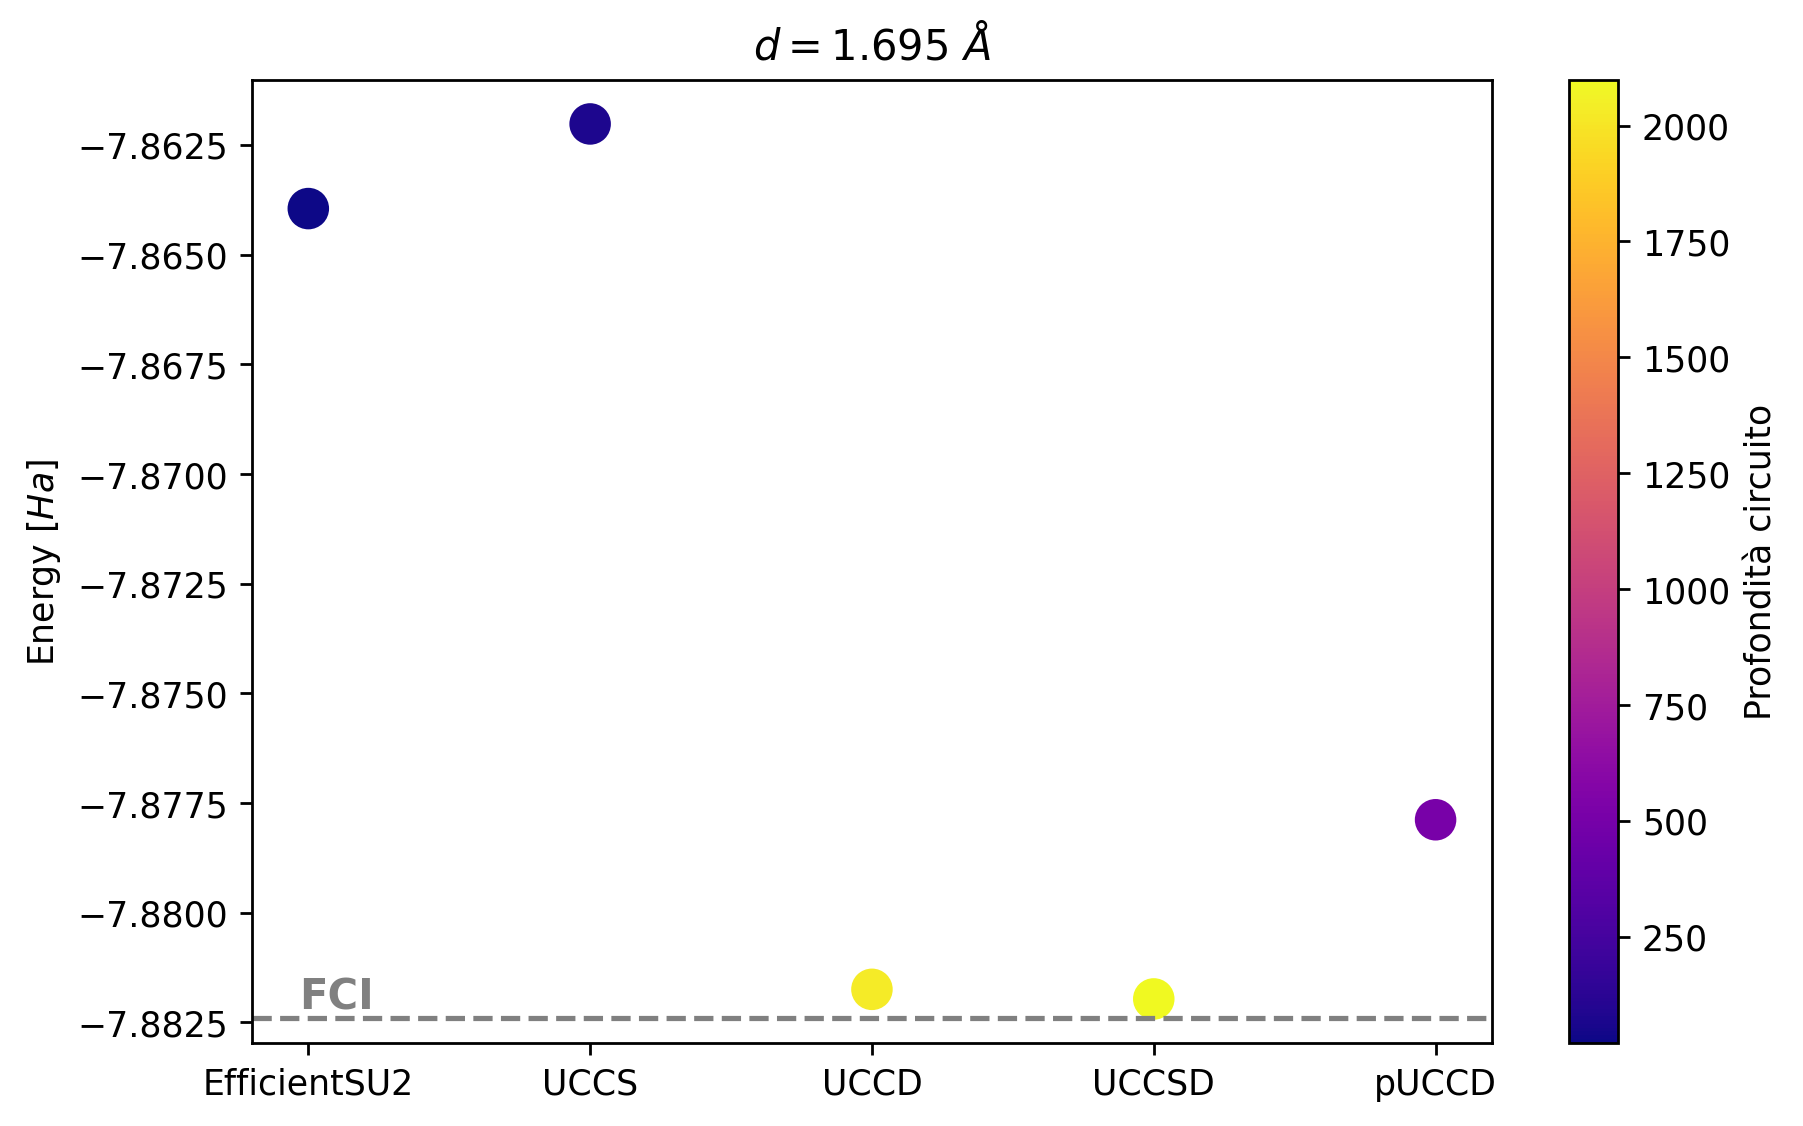
\includegraphics[width=.5\linewidth]{Immagini/Capitolo_3/ground.png}}%
        \hfill
        \subfloat[\centering A grande distanza]{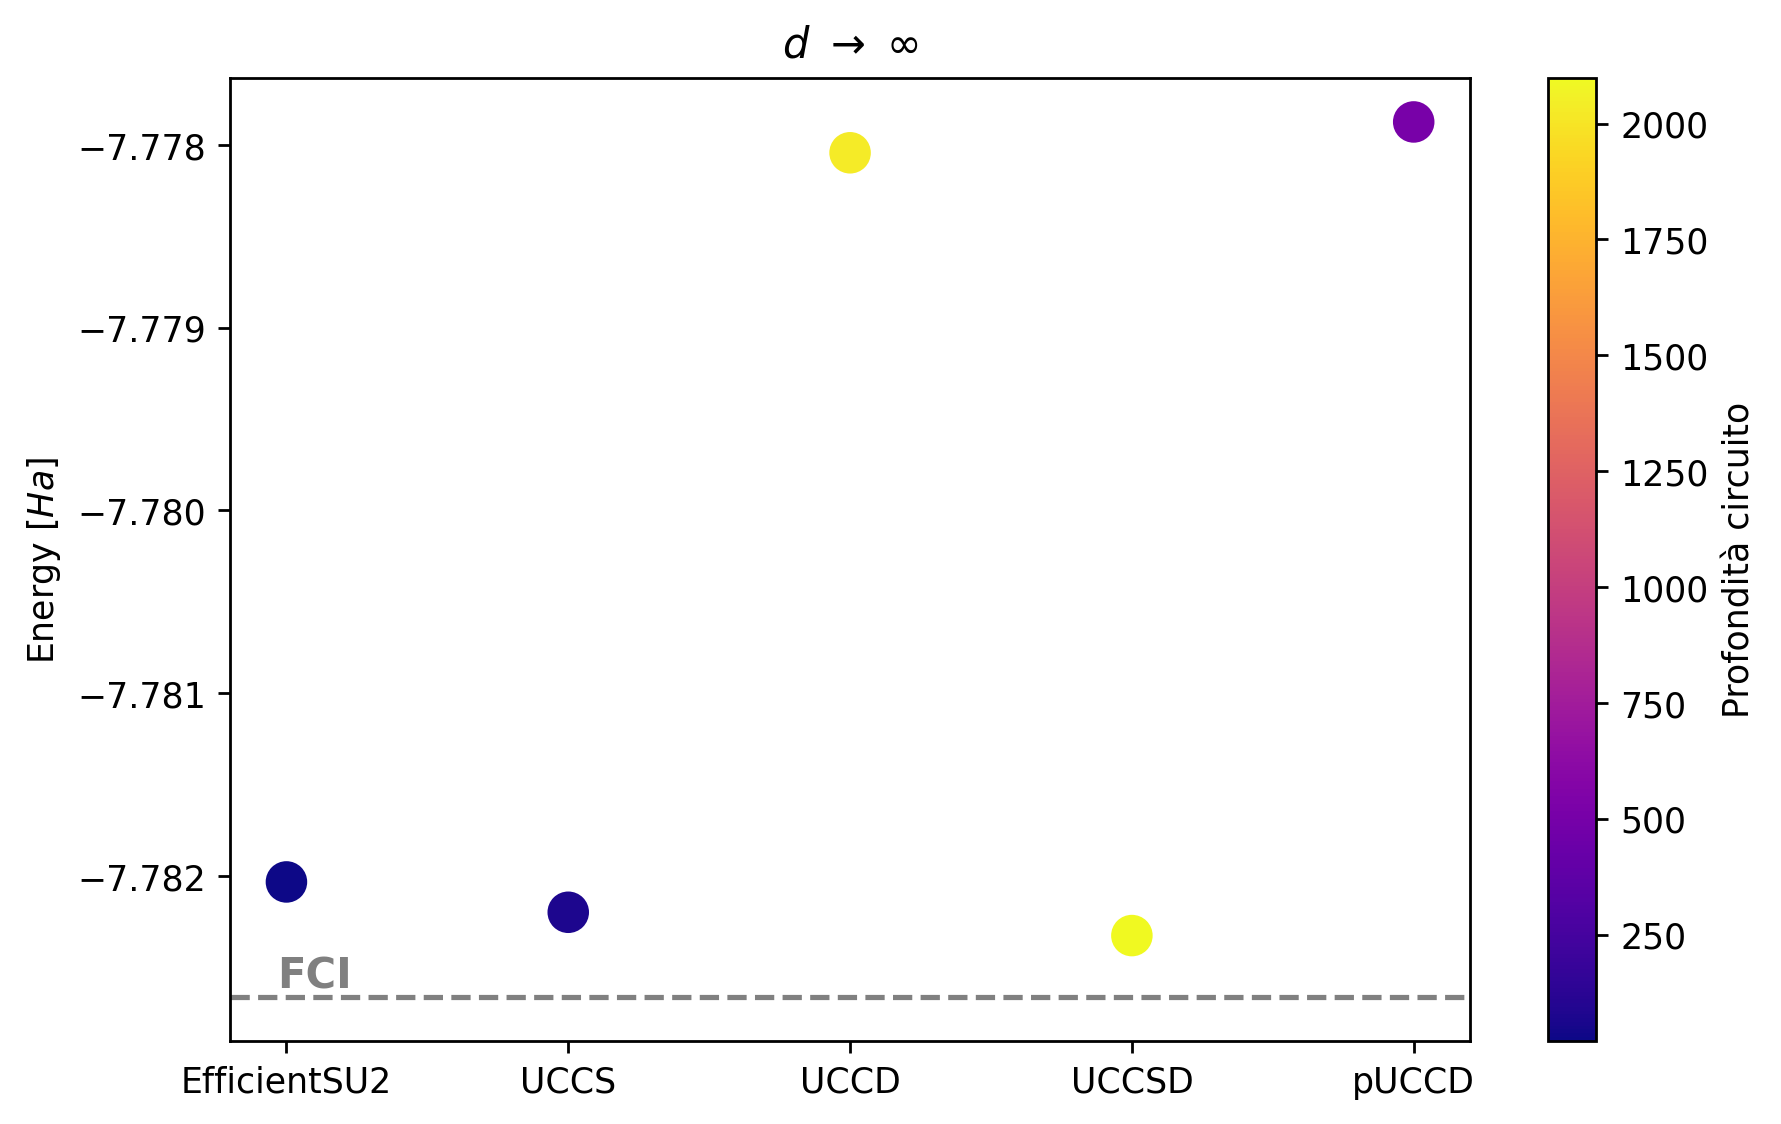
\includegraphics[width=.5\linewidth]{Immagini/Capitolo_3/dissociazione.png}}%
        \caption{LiH: confronto energie e profondità dei circuiti.}%
        \label{fig:energie-profondità-colorbar}%
    \end{figure}
\end{center}

I comportamenti osservati riscontrati possono essere spiegati considerando i tipi di correlazioni elettroniche che ciascuna forma variazionale riesce a rappresentare. Alla distanza di equilibrio, dove gli atomi sono vicini e legati, sono richiesti metodi in grado di descrivere con precisione le complesse interazioni elettroniche che caratterizzano il legame chimico. Qui gli ansatze che includono eccitazioni doppie, come $q$-UCCD e $q$-UCCSD, catturano meglio le influenze reciproche e pertanto forniscono stime di energia più accurate.
In fase di dissociazione, invece, gli elettroni diventano progressivamente più indipendenti. La correlazione elettronica è meno intensa e un metodo semplice come $q$-UCCS può descrivere in modo adeguato la situazione, anche se include solo eccitazioni singole. Questo perché, all’infinito, la mancanza di interazione tra gli elettroni fa sì che la descrizione dell’energia totale non richieda una struttura complessa.
$q$-UCCSD, che comprende eccitazioni singole e doppie, è in grado di bilanciare le esigenze di complessità del legame e la semplicità della dissociazione, combinando i vantaggi degli altri due.

Infine, $q$-pUCCD mostra contemporaneamente una sovrastima nel valore dell'energia all'equilibrio e, poiché anch'esso trascura le eccitazioni del primo ordine, anche nel valore di $E_\infty$. Tuttavia, esiste una tecnica capace di portare un miglioramento significativo alle stime prodotte da $q$-pUCCD, soprattutto per quanto riguarda la descrizione della dissociazione: l'\textbf{ottimizzazione orbitale}, introdotta nella Sezione~\ref{subsec:pUCCD}, che mitiga in parte l'iniziale esclusione delle \inglese{singles}.

% --------------------------------------------------------------------------------------------------------------
\subsection{Analisi del processo di ottimizzazione}

Per ogni ansatz, il processo di ottimizzazione dell’energia a una distanza fissa di $d=1.595$ \AA~è stato valutato analizzando:
\begin{itemize}
    \item la varianza dei valori campionati durante l’ottimizzazione;
    \item la massima distanza tra il valore di convergenza e i valori provati.
\end{itemize}

La Figura~\ref{fig:LiH-UCC-ottimizzazione} illustra l’andamento dell’ottimizzazione per ciascun ansatz, mentre i valori numerici sono riportati nella Tabella \ref{tab:ottimizzazione}:

\begin{figure}[H]
    \centering
    \hspace{-0.9cm}
    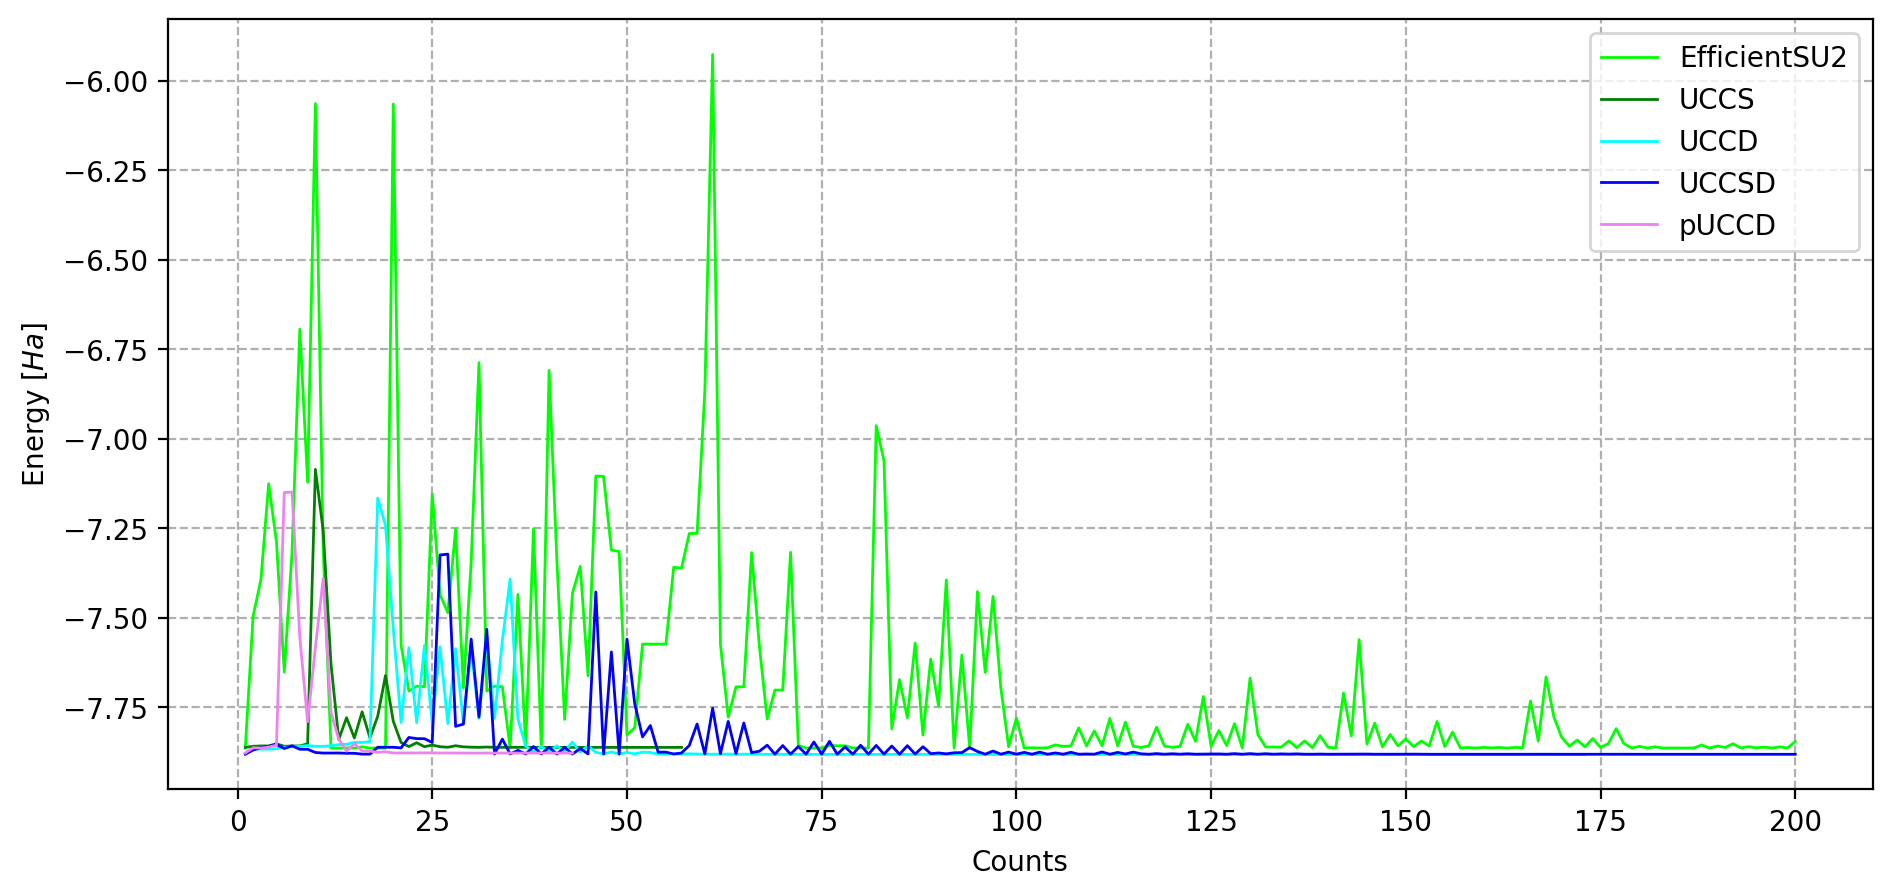
\includegraphics[width=.8\linewidth]{Immagini/Capitolo_3/ottimizzazione.png}
    \caption{LiH: processo di ottimizzazione a $d=1.595$ \AA.}
    \label{fig:LiH-UCC-ottimizzazione}
\end{figure}


\begin{table}[H]
    \centering
    \begin{tabular}{|c|c|c|}
    \hline
    \textbf{Ansatz}                              & \textbf{Varianza (Ha$^2$)} & \textbf{Massima $\Delta E$ (Ha)} \\ \hline
    {\color[HTML]{32CB00} \textbf{EfficientSU2}} & 0.1       & 1.9        \\ \hline
    {\color[HTML]{036400} \textbf{UCCS}}         & 0.02      & 0.8        \\ \hline
    {\color[HTML]{34CDF9} \textbf{UCCD}}         & 0.01      & 0.7        \\ \hline
    {\color[HTML]{3531FF} \textbf{UCCSD}}        & 0.006     & 0.6        \\ \hline
    {\color[HTML]{D952D8} \textbf{pUCCD}}        & 0.03      & 0.7        \\ \hline
\end{tabular}
\caption{Varianza e massima distanza nel processo di ottimizzazione.}
\label{tab:ottimizzazione}
\end{table}


L'ansatz \inglese{hardware-efficient} mostra una varianza significativamente più alta (0.1~Ha$^2$) rispetto alle varianti $q$-UCC, suggerendo che esso vada ad esplorare un’area più ampia dello spazio dei parametri durante l’ottimizzazione. Data la sua natura \inglese{problem agnostic}, ciò potrebbe significare che nella ricerca vengono incluse anche delle regioni non interessanti in senso fisico, portando a una minore stabilità. D'altra parte, negli ansatze $q$-UCC la varianza è decisamente più bassa: da tre volte minore per $q$-pUCCD ($0.03$~Ha) fino a quasi venti volte più piccola per $q$-UCCSD ($0.006$~Ha). Ciò potrebbe indicare un’esplorazione più localizzata intorno al minimo energetico, con un maggiore focus sulle regioni fisicamente significative. Tuttavia, questa focalizzazione non garantisce necessariamente una maggiore stabilità: anche in simulazioni ideali è stato necessario ripetere più volte il processo di ottimizzazione per ottenere risultati consistenti, segnalando un'alta sensibilità ai parametri iniziali e rappresentando una sfida per applicazioni su dispositivi rumorosi.

Lo stesso comportamento si osserva nella distanza massima tra valore di convergenza e valori provati. In questo caso, EfficientSU(2) presenta una distanza massima molto alta, di circa $2$~Ha. Questo è coerente con una maggiore ampiezza nell’esplorazione dello spazio dei parametri, che potrebbe risultare vantaggiosa per evitare minimi locali, ma può aumentare la possibilità di risultati devianti. Al contrario, $q$-UCCSD presenta la distanza minore (0.6 Ha), indicativa di una ricerca più mirata e di una maggiore costanza nella convergenza verso il minimo globale. Tuttavia, proprio questa localizzazione dei minimi può rendere più probabile che l’ottimizzazione si arresti prematuramente, prima di raggiungere il vero minimo assoluto, specialmente in presenza di rumore. Lo stesso discorso si applica anche alle altre varianti \inglese{Coupled Cluster}, che mostrano diverge massime sempre nell'ordine dei decimi di hartree: $0.7$~Ha per $q$-UCCD e $q$-pUCCD, $0.8$~Ha per $q$-UCCS.

In generale, gli ansatze con una varianza più bassa e una distanza massima minore tendono a raggiungere il minimo più rapidamente, mentre EfficientSU(2) potrebbe richiedere più iterazioni a causa della maggiore ampiezza esplorativa. Anche se il numero di iterazioni e il tempo di ottimizzazione dipendono dalla potenza di calcolo disponibile, questo rimane un dato interessante per valutare l’efficienza degli ansatze in contesti pratici.


% ==============================================================================================================
\section{Orbital optimized \textit{q}-pUCCD}\label{sez:orbital-optimization}

In questa sezione viene illustrata l’implementazione di un circuito $q$-oo-pUCCD basato sull’ottimizzazione orbitale. Si parte dalla costruzione teorica dell’operatore di rotazione $\hat{\mathcal{K}}$ per modificare la base degli orbitali, adattando dinamicamente gli integrali dell'hamiltoniana per ogni iterazione del processo VQE. Questo approccio ottimizza direttamente la forma della funzione d’onda e permette di esplorare configurazioni che minimizzano l’energia dell’ansatz scelto. 

% --------------------------------------------------------------------------------------------------------------
\subsection{Costruzione del circuito \textit{q}-oo-pUCCD}\label{subsec:costruzione-oo-pUCCD}

Per implementare attraverso un circuito l'operatore $e^{\hat{\mathcal{K}}}$ si parte dal considerare le possibili rotazioni di coppie di orbitali di spin, cioè le entrate non nulle della matrice anti-hermitiana $\hat{\mathcal{K}}$ introdotta in Sezione~\ref{eqn:ansatz-oo-pUCCD}, qui sotto riportata:

\begin{equation*}
    \hat{\mathcal{K}} = \sum_{p<q} \mathcal{K}_{pq} (a_{q}^{\dagger}a_{p} - a_{p}^{\dagger}a_{q})
\end{equation*}

La funzione \myinline{create_orbital_rotation_list} genera la lista ordinata delle rotazioni tra orbitali con indici $p<q$, nella forma \myinline{[0,1]}, \myinline{[0,2]} e così via.

% orbital opt ___________________________________________________
\begin{tcolorbox}[title=Generazione lista di eccitazioni]
\begin{lstlisting}
def create_orbital_rotation_list(ansatz) -> list:

half_as = int(ansatz.num_qubits / 2)
orbital_rotations = []

for i in range(half_as):
        for j in range(half_as):
            if i < j:
                orbital_rotations.append([i, j])
                
return orbital_rotations
\end{lstlisting}
\vspace{-0.2cm}
\end{tcolorbox}

Successivamente, si converte ogni coppia di indici $(p,q)$ in un operatore fermionico $a^{\dagger}_{q} a_p$ con la funzione \myinline{build_fermionic_excitation_ops}
    
% orbital opt ___________________________________________________
\begin{tcolorbox}[title=Costruzione operatore fermionico, breakable]
\begin{lstlisting}
def build_fermionic_excitation_ops(
    mo_problem, 
    excitations: Sequence,
    mapper: QubitMapper = JordanWignerMapper()
    ) -> list[FermionicOp]:
    
    num_spin_orbitals = 2 * mo_problem.num_spatial_orbitals
    operators = []

    for exc in excitations:
        label = []
        for occ in exc[0]:
            label.append(f"+_{occ}")
        for unocc in exc[1]:
            label.append(f"-_{unocc}")
        op = FermionicOp({" ".join(label): 1}, num_spin_orbitals=num_spin_orbitals)
        op_adj = op.adjoint()
        # va considerata una fase immaginaria introdotta dalla approssimazione di 
        # Trotter implementata in Qiskit

        op_minus = 1j * (op - op_adj)
        operators.append(op_minus)
        
        # map to qubit operators
        qubit_ops = mapper.map(operators)

    return qubit_ops
\end{lstlisting}
\vspace{-0.2cm}
\end{tcolorbox}

Infine, si usa la classe \myinline{EvolvedOperatorAnsatz} per costruire il circuito con le eccitazioni esponenziate. Quest'ultimo va poi concatenato a $q$-pUCCD, passato in argomento come \myinline{initial_state}, per formare $q$-oo-pUCCD.

% orbital opt ___________________________________________________
\begin{tcolorbox}[title=Generazione ansatz oo-pUCCD, breakable]
\begin{lstlisting}
def generate_oo_puccd (puccd, mo_problem, excitations):

    qubit_ops = build_fermionic_excitation_ops(
        mo_problem, 
        excitations
        )

    oo_puccd = EvolvedOperatorAnsatz(
        operators=qubit_ops,
        initial_state=puccd,
        parameter_prefix='k'
    )

    bounds = [[-np.pi,np.pi] for _ in range(
             oo_puccd.num_parameters)]
    oo_puccd.parameter_bounds = bounds

    return oo_puccd
\end{lstlisting}
\vspace{-0.2cm}
\end{tcolorbox}


% --------------------------------------------------------------------------------------------------------------
\subsection{oo-VQE}\label{sez:oo-VQE}

L'operazione di ottimizzazione orbitale avviene in concomitanza con VQE, motivo per cui spesso ci si riferisce questo algoritmo con la sigla oo-VQE: durante la minimizzazione dell'energia si ricalcola l'hamiltoniana ad ogni ottimizzazione dei parametri. Per poterlo fare, bisogna accedere agli integrali a uno e due corpi, contenuti nell'attributo \myinline{hamiltonian} dell'\myinline{ElectronicStructureProblem} in forma di classe, un oggetto chiamato \myinline{ElectronicIntegrals}. Al suo interno, gli integrali sono divisi per spin, perciò occorrono due matrici: $\hat{\mathcal{K}}_\alpha$ e $\hat{\mathcal{K}}_\beta$, costruite sempre a partire dalla lista di eccitazioni \myinline{orbital_rotations}. 
La funzione \myinline{orbital_rotation_matrix} riceve in argomento i parametri restituiti da ciascuna interazione del ciclo VQE e li inserisce all'interno delle matrici $\hat{\mathcal{K}}$, quindi restituisce gli operatori di rotazione $e^{\hat{\mathcal{K}}_\alpha}$, $e^{\hat{\mathcal{K}}_\beta}$.

% orbital opt ___________________________________________________
\begin{tcolorbox}[title=Costruzione $e^{\hat{\mathcal{K}}}$, breakable]
\begin{lstlisting}
def orbital_rotation_matrix(
    problem, 
    parameters: np.ndarray, 
    rotations: list
    ) -> Tuple[np.ndarray, np.ndarray]:

    dim_kappa_matrix = problem.num_spatial_orbitals
    
    k_matrix_alpha = np.zeros((dim_kappa_matrix, dim_kappa_matrix))
    k_matrix_beta  = np.zeros((dim_kappa_matrix, dim_kappa_matrix))
    
    for i, exc in enumerate(rotations):
        k_matrix_alpha[exc[0]][exc[1]] =  parameters[i]
        k_matrix_alpha[exc[1]][exc[0]] = -parameters[i]
        k_matrix_beta[exc[0]][exc[1]]  =  parameters[i]
        k_matrix_beta[exc[1]][exc[0]]  = -parameters[i]

    matrix_a = expm(k_matrix_alpha)
    matrix_b = expm(k_matrix_beta)
    
    return matrix_a, matrix_b
\end{lstlisting}
\vspace{-0.2cm}
\end{tcolorbox}

Dopodiché si può procedere con la modifica degli integrali, utilizzando le relazioni \ref{eqn:trasformazione-integrali}. Queste vengono implementate utilizzando \myinline{numpy} per ottimizzare il calcolo il più possibile, dal momento che il numero di moltiplicazioni richieste scala come $\mathcal{O}(K^4)$, con $K$ numero di orbitali spaziali. 
In realtà, nello specifico del caso di $q$-pUCCD, \myinline{ElectronicIntegrals} contiene soltanto valori associati a spin $\alpha$, pertanto \myinline{matrix_b} può essere ignorata. 
Una volta effettuate le trasformazioni degli integrali, si può andare ad estrarre la nuova hamiltoniana di seconda quantizzazione (eq. \ref{eqn:hamiltoniana-seconda-q}) dal problema elettronico ruotato.

% orbital opt ___________________________________________________
\begin{tcolorbox}[title=Rotazioni orbitali, breakable]
\begin{lstlisting}
def rotate_orbitals(
    problem, 
    one_body, 
    two_body, 
    matrix_a, 
    matrix_b, 
    mapper = JordanWignerMapper()
    ): 

    C = matrix_a  # Matrice C = exp(K_a)

    N = len(C)

    # Trasformazione degli integrali a un corpo
    one_body_transformed = np.einsum('up,uv,vq->pq', C, one_body, C)
    # Trasformazione degli integrali a due corpi
    eri_transformed = np.einsum('up,vq,xr,ys,uvxy->pqrs', C, C, C, C, eri)
    eri_transformed = np.zeros((N, N, N, N))
    # Definizione di un oggetto ElectronicIntegrals per modificare quello contenuto in problem
    e_int = ElectronicIntegrals.from_raw_integrals(
        h_transformed,                                            
        eri_transformed
    )

    problem.hamiltonian.ElectronicIntegrals = e_int

    # extract rotated operator
    rotated_operator = problem.hamiltonian.second_q_op()
    rotated_operator = mapper.map(rotated_operator)

    return rotated_operator
\end{lstlisting}
\vspace{-0.2cm}
\end{tcolorbox}

Su questo \myinline{rotated_operator} sarà calcolato il valore di aspettazione (eq. \ref{eqn:energia-oo-pUCCD}) nel ciclo successivo di VQE, nel quale saranno ottimizzati ulteriormente i parametri, che poi saranno usati per generare una nuova matrice di rotazione; questo procedimento quindi continua fino a convergenza.

% --------------------------------------------------------------------------------------------------------------
\subsection{Risultati}\label{sez:risultati-oo-pUCCD}

In questa sezione si riportano i risultati ottenuti applicando l’ottimizzazione orbitale nella simulazione delle molecole LiH e H$_2$O, per osservare il comportamento di questo approccio su un sistema più complesso, evidenziando eventuali limiti e vantaggi scalabili a sistemi di dimensioni maggiori.

% ..............................................................................................................
\subsubsection{LiH}

Nel caso dell'idruro di litio, il circuito $q$-oo-pUCCD comporta un aumento in profondità di solamente 155, il che renderebbe questo ansatz estremamente promettente, se fosse anche capace di migliorare sensibilmente i risultati di pUCCD. In realtà, per quanto riguarda l'energia di stato fondamentale, è osservata una diminuzione del valore calcolato, ma non di certo degna di nota. Il valore di energia a grandi distanze invece giova della correzione, compatibilmente con quanto osservato in altri studi \cite{Sokolov_2020,Zhao_2023}, anche se non nella stessa misura.

\begin{figure}[H]
    \centering
    \hspace{-1cm}
    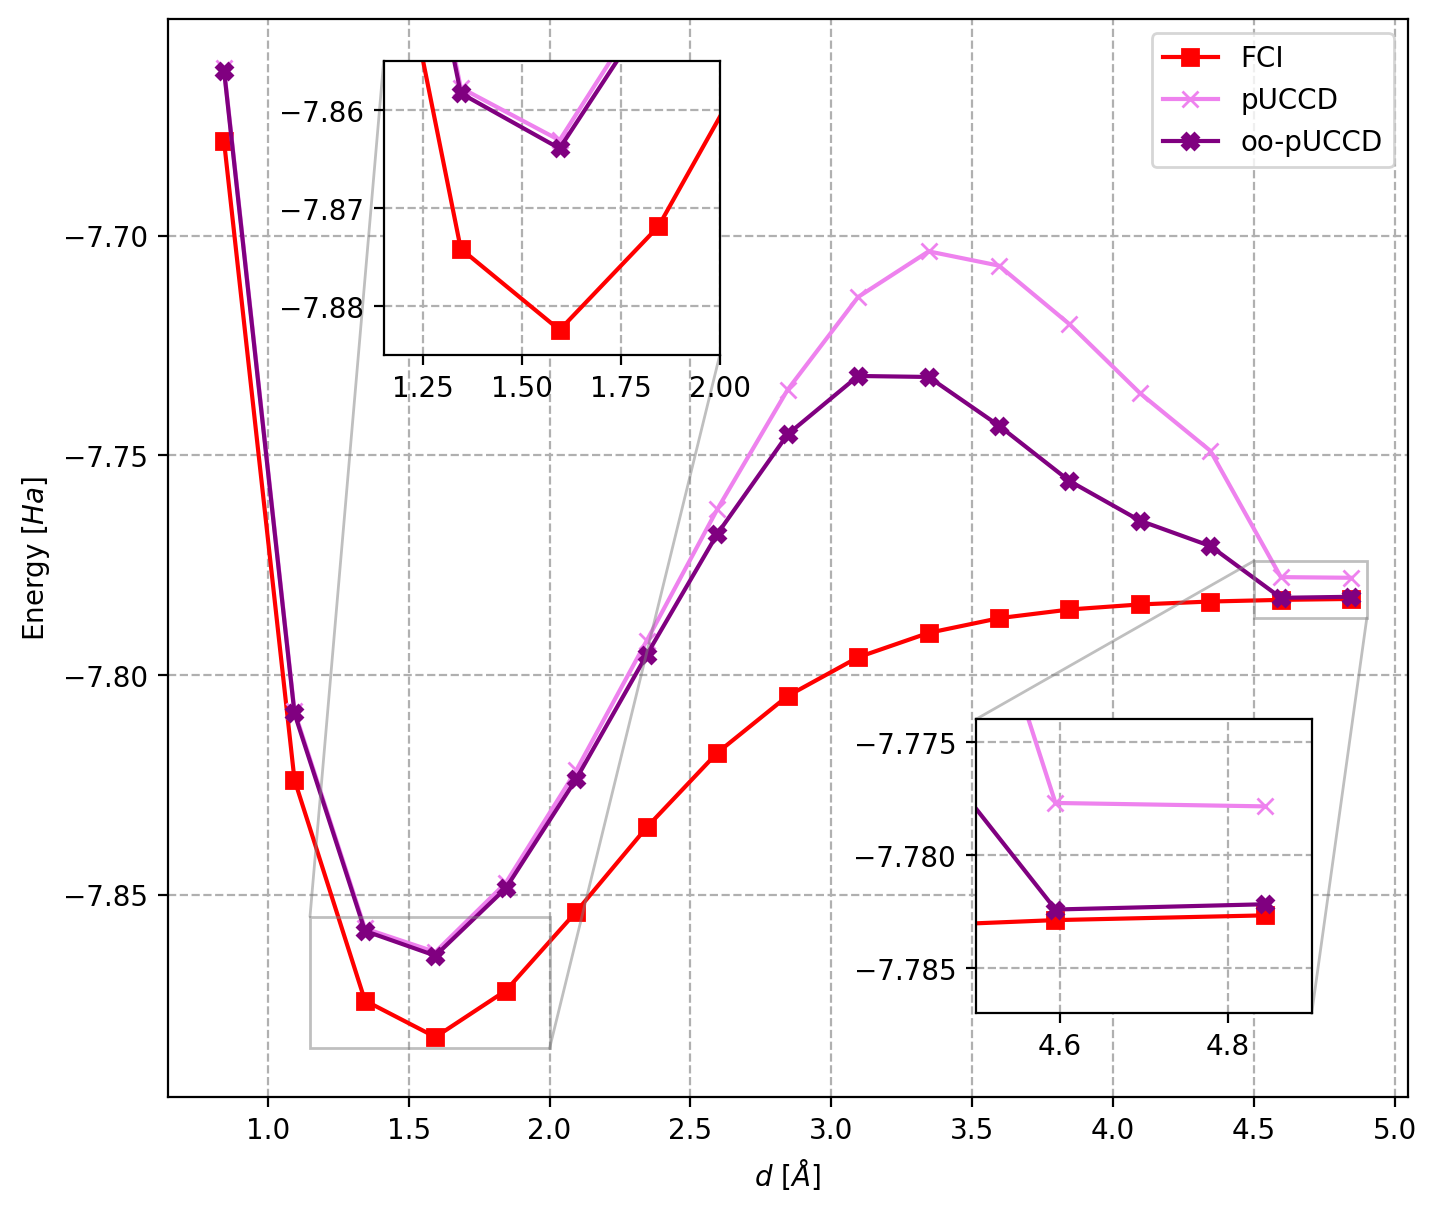
\includegraphics[width=.6\linewidth]{Immagini/Capitolo_3/LiH_oo_pUCCD.png}
    \caption{LiH: $q$-pUCCD con ottimizzazioni orbitali.}
    \label{fig:LiH-ottimizzazioni-orbitali}
\end{figure}

% Please add the following required packages to your document preamble:
% \usepackage[table,xcdraw]{xcolor}
% Beamer presentation requires \usepackage{colortbl} instead of \usepackage[table,xcdraw]{xcolor}
\begin{table}[H]
    \centering
    \begin{tabular}{|c|c|c|c|c|c|c|}
    \hline
    \textbf{Metodo}                                              & \textbf{Depth} & \textbf{CNOT} & \textbf{Parametri} & \textbf{$E_0$} & \textbf{$E_\infty$} & \textbf{$\Delta E_{\text{max}}$} \\ \hline
    \textbf{\color[HTML]{CB0000} FCI}       & /              & /             & /                  & -7.8824        & -7.7827             & /                                \\ \hline
    \textbf{\color[HTML]{D952D8} $q$-pUCCD} & 511            & 384           & 4                  & -7.8630        & -7.7779             & 0.09                             \\ \hline
    \textbf{\color[HTML]{6200C9} $q$-oo-pUCCD}               & 666           & 464           & 14                 & -7.8639        & -7.7822             & 0.06                             \\ \hline
\end{tabular}
\caption{Energie calcolate in hartree e dimensioni circuiti oo-LiH.}
\label{tab:oo-LiH}
\end{table}

La differenza nei minimi di energia tra $q$-pUCCD e $q$-oo-pUCCD è di appena $0.8$~mHa, come riportato nella Tabella~\ref{tab:oo-LiH}, mentre a grande distanza raggiunge i $15$~mHa, abbassando la deviazione dal valore di riferimento FCI a soltanto $0.5$~mHa.


% ..............................................................................................................
\subsubsection{H$_2$O}

Per testare ulteriormente le potenzialità dell'algoritmo oo-VQE, si applica ad un sistema più laborioso: la molecola di H$_2$O.
Anche in questo caso si utilizza \myinline{FreezeCoreTransformer} per ridurre la dimensione del problema, che stavolta porta all'esclusione di due orbitali \inglese{core}. La differenza in profondità tra i circuiti si fa più marcata rispetto a LiH, con $q$-oo-pUCCD che contiene oltre $250$ \inglese{layers} in più dei circa $1100$ di pUCCD. Tuttavia, si tratta ancora di un circuito piuttosto contenuto, soprattutto considerando che $q$-UCCSD per lo stesso problema supererebbe una profondità di $10000$.

\begin{figure}[H]
    \centering
    \hspace{-1cm}
    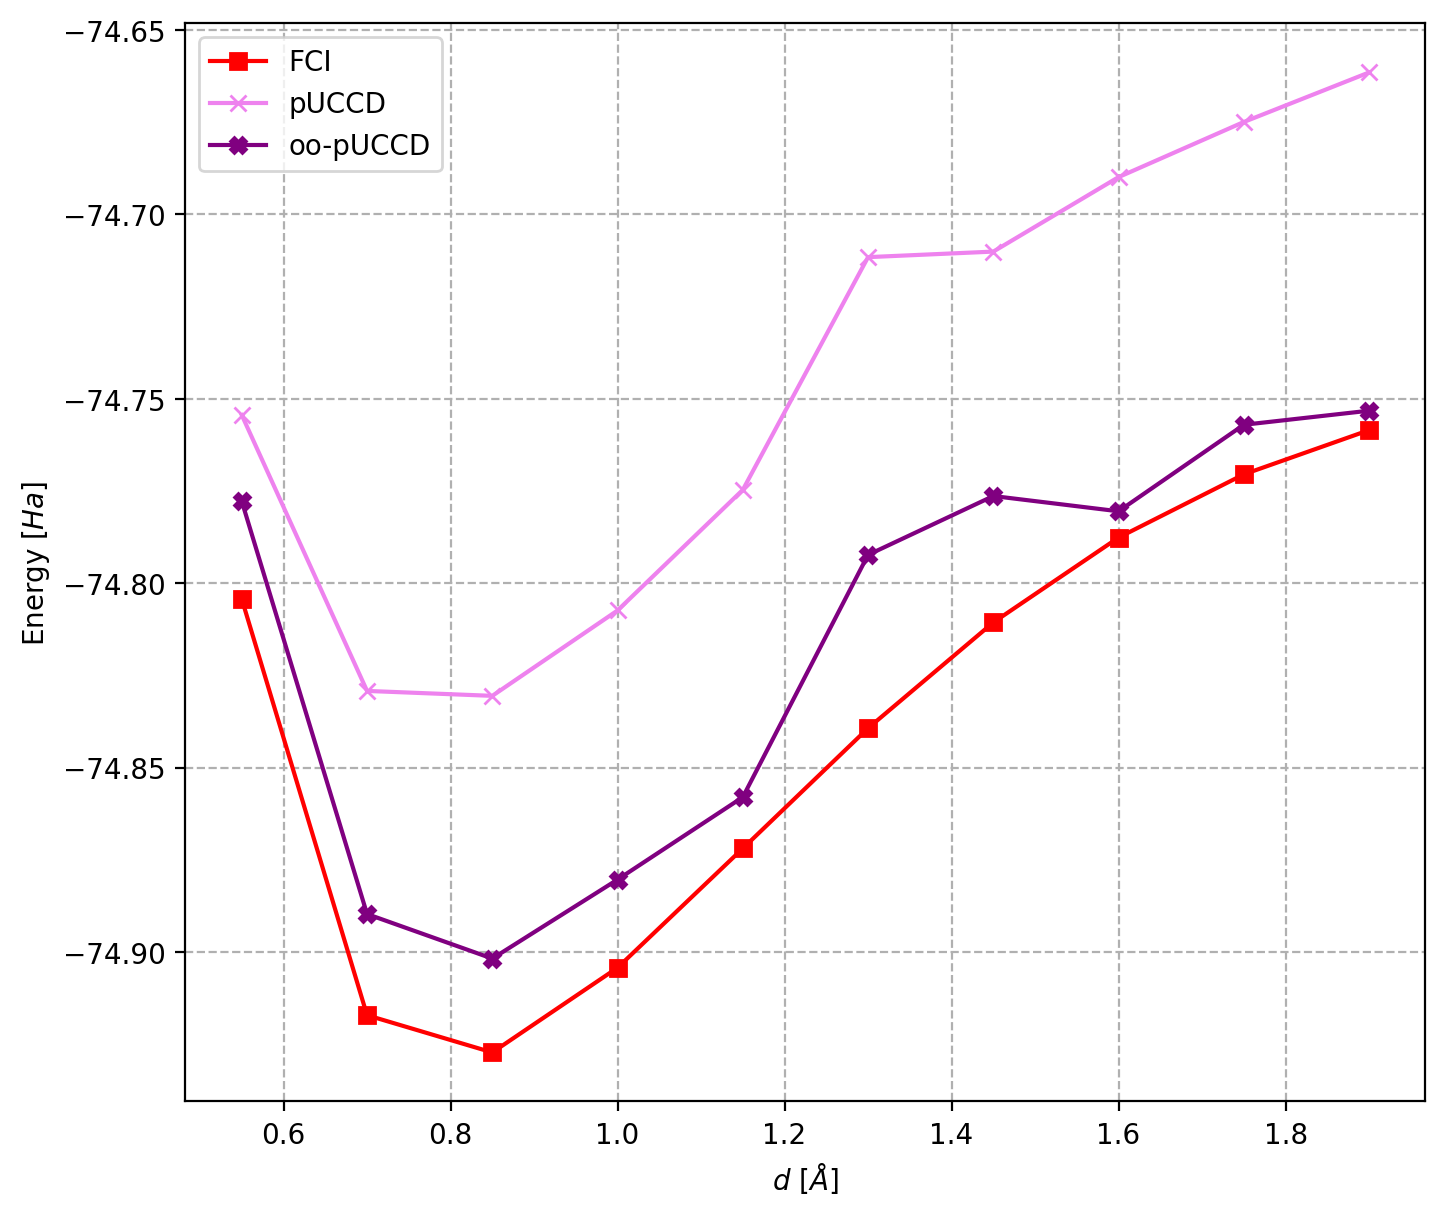
\includegraphics[width=.6\linewidth]{Immagini/Capitolo_3/H2O_oo_pUCCD.png}
    \caption{H$_2$O: $q$-pUCCD con ottimizzazioni orbitali.}
    \label{fig:H2O-ottimizzazioni-orbitali}
\end{figure}

% Please add the following required packages to your document preamble:
% \usepackage[table,xcdraw]{xcolor}
% Beamer presentation requires \usepackage{colortbl} instead of \usepackage[table,xcdraw]{xcolor}
\begin{table}[H]
    \centering
    \begin{tabular}{|c|c|c|c|c|c|}
    \hline
    \textbf{Metodo} & \textbf{Depth} & \textbf{CNOT} & \textbf{Parametri} & \textbf{$E_0$} & \textbf{$\Delta E_{\text{max}}$} \\ \hline
    \textbf{\color[HTML]{CB0000} FCI}           & /      & /      & /     & -74.927   & /       \\ \hline
    \textbf{\color[HTML]{D952D8} $q$-pUCCD}     & 1145   & 896    & 8     & -74.831   & 0.13    \\ \hline
    \textbf{\color[HTML]{6200C9} $q$-oo-pUCCD}  & 1396   & 1036   & 23    & -74.902   & 0.05    \\ \hline
\end{tabular}
\caption{Energie calcolate in hartree e dimensioni circuiti oo-H$_2$O.}
\label{tab:oo-H2O}
\end{table}

In questo caso, osservando la Figura~\ref{fig:H2O-ottimizzazioni-orbitali} e la Tabella~\ref{tab:oo-H2O}, il vantaggio offerto dalle ottimizzazioni orbitali nel calcolo dell'energia è lampante: il minimo diminuisce di oltre $70$~mHa, il valore a grandi distanze scende fino a discostarsi di soli $5$~mHa dal valore FCI. Oltre a questo, l’ottimizzazione orbitale permette di recuperare una frazione significativa del valore assoluto corretto dell’energia totale a tutte le geometrie studiate, mantenendo una precisione entro $10$~mHa rispetto ai calcoli di riferimento e riproducendo, almeno qualitativamente, i profili energetici corretti.

Riassumendo, questi risultati suggeriscono l'ansatz $q$-oo-pUCCD può offrire un sensibile miglioramento nella precisione energetica, particolarmente significativo nelle energie a lungo raggio. Allo stesso tempo, l’incremento di profondità si mantiene limitato, soprattutto in confronto agli ansatz UCC più strutturati. In particolare, nel caso di H$_2$O, si osserva un miglioramento sostanziale sia a grandi distanze che nella zona del minimo, rendendo il metodo interessante per applicazioni future, nelle quali potrebbe costituire un approccio bilanciato fra una buona approssimazione energetica e una complessità circuitale contenuta.

% Conclusioni
\addcontentsline{toc}{chapter}{Conclusioni} % Capitolo numerato?

\chapter*{Conclusioni}
% ==============================================================================================================
% Commento al lavoro svolto

Nel presente lavoro, è stata esplorata la capacità degli ansatze \inglese{quantum Unitary Coupled Cluster} ($q$-UCC) di riprodurre con precisione le energie fondamentali e di dissociazione della molecola di idruro di litio (LiH), con un focus sulla complessità circuitale richiesta da ciascuna variante. I metodi studiati, inclusi $q$-UCCS, $q$-UCCD, $q$-UCCSD, $q$-pUCCD e EfficientSU(2), hanno permesso di valutare i compromessi tra accuratezza energetica e profondità circuitale, un aspetto cruciale per una possibile implementazione su \inglese{quantum processing units} (QPU) attuali.

L’analisi ha messo in luce le peculiarità di ciascun ansatz: se da un lato $q$-UCCSD è stato il più accurato, producendo risultati molto vicini alla soglia teorica data dal modello classico Full Configuration Interaction (FCI), dall’altro richiede una profondità circuitale elevata e un numero di porte CNOT significativo, che ne limita la praticità per implementazioni hardware immediate. Al contrario, EfficientSU(2), con una struttura circuitale semplificata, ha dimostrato di poter fornire stime energetiche accettabili per determinate condizioni, nonostante richieda risorse minime. L’introduzione del \inglese{quantum} pair-UCCD ($q$-pUCCD) e delle ottimizzazioni orbitali ($q$-oo-pUCCD) ha inoltre indicato una promettente via intermedia tra la precisione e la riduzione del costo computazionale, posizionandosi come opzione interessante per simulazioni molecolari in cui le risorse quantistiche siano limitate.

Complessivamente, i risultati ottenuti offrono spunti sul potenziale degli ansatze $q$-UCC per simulazioni chimiche avanzate, sebbene l’attuale tecnologia richieda la continua ricerca di una maggiore efficienza circuitale. Questo studio potrebbe suggerire che sia possibile ottenere risultati significativi anche con architetture hardware contenute, grazie a scelte ponderate di ansatz e a ottimizzazioni.
% ==============================================================================================================
% Prospettive future
Alla luce di questi risultati, sviluppi futuri potrebbero orientarsi verso la valutazione degli ansatze in contesti più realistici. Un primo passo potrebbe essere quello di testare le configurazioni $q$-UCC attraverso simulatori quantistici con rumore, che permetterebbero di comprendere meglio l’effetto degli errori di gate e delle fluttuazioni di stato sulle stime energetiche. Questa fase sarebbe cruciale per determinare la robustezza degli ansatze rispetto agli errori di calcolo e per identificare potenziali limiti nelle implementazioni circuitali attuali.

Successivamente, e qualora i risultati su simulatori rumorosi confermassero la stabilità delle soluzioni, si potrebbe prevedere un test diretto su hardware quantistico. Tale verifica consentirebbe di validare le stime energetiche ottenute e di confrontare l’effettiva complessità circuitale con le capacità dei dispositivi fisici, aprendo la strada a simulazioni sperimentali più accurate e, eventualmente, a miglioramenti nelle strategie di ottimizzazione e nella selezione degli ansatze per applicazioni pratiche.


\clearpage

%================================================================== Fine MAINMATTER

%------------------------------------------------------------------ Inizio BACKMATTER

% Appendici?
%\input{Organizzazione Files/Appendici/Appendice}

% Bibliografia
\printbibliography

%------------------------------------------------------------------

% Ringraziamenti?
%\addcontentsline{toc}{chapter}{Ringraziamenti} % Capitolo non numerato
%\input{Organizzazione Files/Ringraziamenti}

%==================================================================
\end{document}
